\documentclass[UTF8]{ctexart}
\usepackage{geometry}
\usepackage{amsmath, amssymb, amsthm}
\usepackage{graphicx}
\usepackage{booktabs}
\usepackage{hyperref}
\usepackage{cases}
\usepackage{physics}
\usepackage{bm}

\geometry{a4paper, margin=2.5cm}

\usepackage{hyperref}
\hypersetup{colorlinks=true, linkcolor=black}
\theoremstyle{definition}
\newtheorem{remark}{注记}

\title{\textbf{热学期末复习笔记}}
\author{周锦添}
\date{\today}

\begin{document}
\maketitle
\tableofcontents
\newpage

% ============================================
\section{第四章：热力学第一定律}
% ============================================

\subsection{热力学过程和准静态过程}

\textbf{热力学过程}：热力学系统的状态随时间的变化称为热力学过程（简称过程）。

\textbf{准静态过程}：进行的足够缓慢，以致于系统连续经过的每一个中间态都可以近似为平衡态的过程。
\begin{itemize}
    \item 在过程进行的每一时刻，系统都有确定的状态参量；
    \item 通过描述状态参量的变化规律就可以很好地描述准静态过程的性质；
    \item \textbf{理想过程}，实际过程都不是严格的准静态过程。
\end{itemize}

对于准静态过程，其连续经过的每一个中间态都可以在 $p$-$V$ 图（或 $T$-$V$ 图、$p$-$T$ 图）中表示为一个点，整个过程可以在 $p$-$V$ 图（或 $T$-$V$ 图、$p$-$T$ 图）中表示为一条曲线。

按状态参量变化特征划分准静态过程：等压过程、等体过程、等温过程、绝热过程……

\subsubsection*{实现准静态过程的可能性及条件}

\textbf{准静态过程近似实现的条件}：系统的\textbf{弛豫时间}远小于过程的特征时间。

例如：气缸活塞系统中气体的膨胀和压缩过程，活塞速度 $\sim 10\,\mathrm{m/s}$，声速 $\sim 300\,\mathrm{m/s}$，可以近似为准静态过程。

\textbf{具体操作}：只要使相应的特征量 $X$ 在每一步中的变化量 $\Delta X$ 小到可近似为无穷小量 $\mathrm{d}X$，这一过程就可近似为准静态过程。

\textbf{气体向真空膨胀，不是准静态过程}。

\begin{remark}
弛豫时间是系统从不平衡态恢复到平衡态所需的特征时间。若外界驱动很慢，系统有足够时间恢复平衡，则过程可视为准静态。
\end{remark}

\begin{figure}[htbp]
\centering
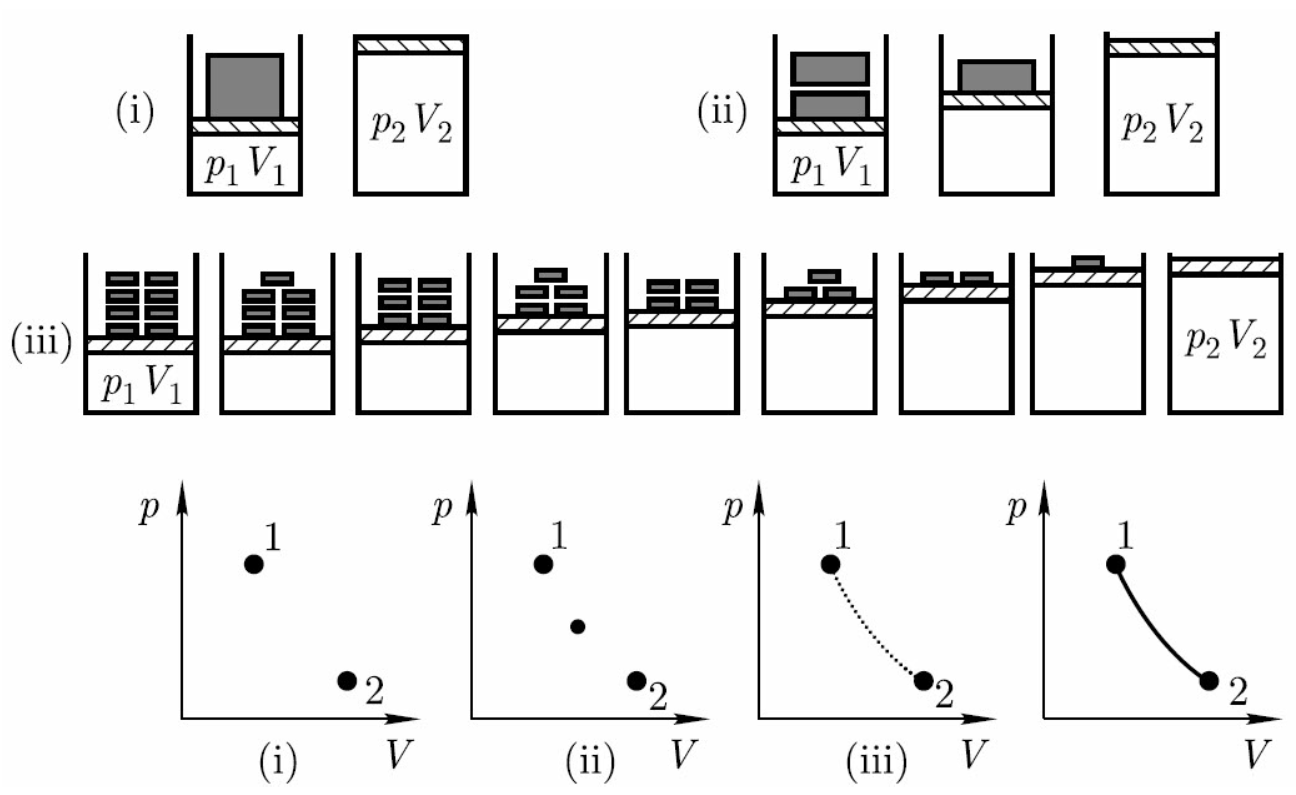
\includegraphics[width=0.6\textwidth]{quasistatic_process.png}
\caption{准静态过程的实现：从有限步到无穷小步的极限（需插入原PPT第3页示意图）}
\label{fig:quasistatic}
\end{figure}

% --------------------------------------------
\subsection{热力学第一定律的建立}
% --------------------------------------------

\subsubsection*{能量守恒定律}

\begin{quote}
有一个事实，那就是有一个到目前为止掌控了我们所知道的自然现象的定律，而这个定律在我们所知范围内没有任何的例外，而且据我们目前所知，它是准确的。这个定律被称为能量守恒。它说明了有一个特定的物理量，我们称之为“能量”。这量在自然状态经历了各种变化后，并不会改变。这是一个最抽象的概念，因为它是一个数学的原理：它说明了有一个数值量在一些事件发生时不会改变。它并不是任何物理过程或者具体事物的描述；它仅仅是一个奇怪的事实：我们可以先对系统计算一些数值，而当系统经历了一些变化之后，我们同样的再去计算那些数值，结果会发现数值和一开始的时候是相同的。

——费曼物理学讲义
\end{quote}

\subsubsection*{能量的历史（简略）}

\begin{itemize}
    \item 能量（energy）源于希腊语 $\varepsilon\nu\varepsilon\rho\gamma\varepsilon\iota\alpha$，公元前4世纪，亚里士多德首次提出；哲学概念。
    \item 莱布尼茨：living force（拉丁语：vis viva），17世纪末，物体质量和其速度平方的乘积，守恒！热能是由物体内的组成物质的运动所构成。
    \item 托马斯·杨（Thomas Young）：首次使用“能量” 1807。
    \item 科里奥利（Gustave-Gaspard Coriolis）：动能 1829；兰金（William John Macquorn Rankine）：势能 1853。
    \item 机械能和热等价：迈尔（Julius Robert von Mayer）1842。
    \item 焦耳（James Prescott Joule）：热功当量，《The Mechanical Equivalent of Heat》1845。
    \item 亥姆霍兹（Hermann Ludwig Ferdinand von Helmholtz）：能量守恒，《On the Conservation of Force》1847。
\end{itemize}

\subsubsection*{不同形式能量之间的转化}

能量的存在及转化形式：机械能、电能、磁能、化学能、引力势能、弹性势能、表面能、热能……它们之间能够\textbf{互相转化}。

\begin{itemize}
    \item 18世纪末：瓦特的蒸汽机，热能 $\Rightarrow$ 机械能
    \item 1800年：伏打电池，化学能 $\Rightarrow$ 电能
    \item 拉瓦锡、李比希提出：食物的化学能 $\Rightarrow$ 动物体热，活动能量
    \item 1821年：塞贝克发现温差电现象，热能 $\Rightarrow$ 电能
    \item 1831年：法拉第发现电磁感应现象，机械能 $\Rightarrow$ 电能
    \item 1840年：焦耳发现电流的热效应，电能 $\Rightarrow$ 热能
\end{itemize}

\textbf{能量守恒定律}：自然界中一切物体都具有能量，能量有多种不同形式，它能从一种形式转化为另一种形式，从一个物体传递给另一个物体，在转化和传递的过程中，能量的总量不变。

% --------------------------------------------
\subsection{功、热量与内能}
% --------------------------------------------

\subsubsection*{功——力学作用下转移的能量}

\textbf{作用形式}：热力学系统中的力学作用形式多样，如：\textbf{压强}、\textbf{表面张力}、\textbf{弹性力}、\textbf{电磁力}等。

\textbf{作用效果}：使热力学系统的\textbf{平衡条件被破坏}，在系统状态变化过程中伴随有\textbf{能量转移}，其形式即：\textbf{作功}。

\textbf{一些常见过程中元功的计算}：
元功是功概念的推广。\\
作用力为广义力，状态变化为广义位移，记 $Y$ 为广义力，$\Delta X$ 为广义位移，则元功为：
\begin{equation}
\Delta W = Y\Delta X
\end{equation}

\textbf{体积功}（无摩擦、准静态过程）：
\begin{equation}
\Delta W = Y\Delta X = p_e S\Delta X = -p_e\Delta V = -p\Delta V
\end{equation}
\begin{itemize}
    \item $\Delta W > 0$，外界对气体作正功（$\Delta V < 0$）
    \item $\Delta W < 0$，气体对外界作正功（$\Delta V > 0$）
\end{itemize}

\textbf{表面张力功}：设 $\sigma$ 为表面张力系数，在表面张力作用下面积的改变量为 $\Delta S$；则其作功为
\begin{equation}
\Delta W = \sigma\Delta S
\end{equation}

\textbf{弹性力功}：设 $T$ 为棒中弹性力，在其作用下，棒长改变了 $\Delta L$，则其作功为
\begin{equation}
\Delta W = T\Delta L
\end{equation}

\textbf{电源电动势作功}：
\begin{equation}
\Delta W = U\Delta q = IR\cdot I\Delta t = I^2R\Delta t
\end{equation}

\subsubsection*{功的性质}

以体积功为例，当系统体积由 $V_i$ 变化到 $V_f$，如果此过程很慢（\textbf{准静态过程}），外界对系统所作总功为
\begin{equation}
W = -\int_{V_i}^{V_f} p_e\,\mathrm{d}V = -\int_{V_i}^{V_f} p\,\mathrm{d}V
\end{equation}

在 $p$-$V$ 图上可表示为过程曲线与横坐标轴之间围出的面积。

\textbf{总功 $W$ 不仅与初、末态相关，而且与过程曲线有关，即与路径有关。所以，功是过程量，不是态函数。}于是，元功常记为无穷小量 $\mathrm{d}W$，而不能记为全微分 $\mathrm{d}\bm{W}$（不满足多元函数中全微分的条件）。

\begin{figure}[htbp]
\centering
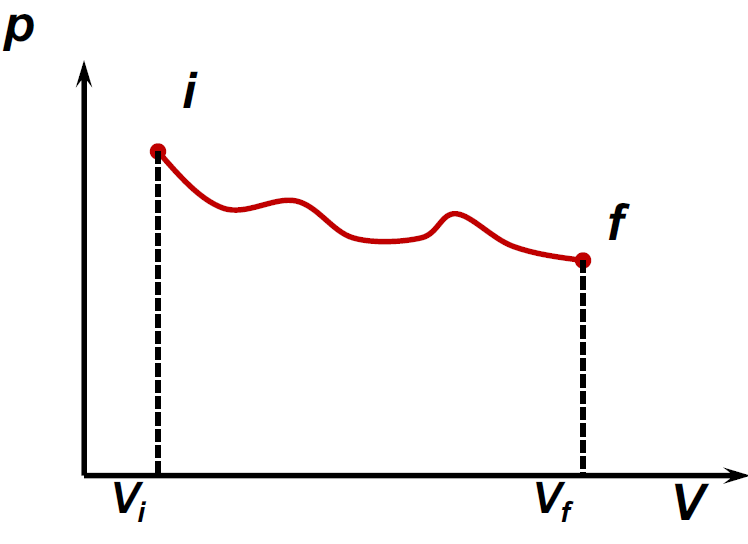
\includegraphics[width=0.5\textwidth]{work_path.png}
\caption{功与路径有关——$p$-$V$ 图上曲线下的面积（需插入原PPT第12次课第10页示意图）}
\label{fig:workpath}
\end{figure}

\subsubsection*{热量——热学作用下转移的能量}

\textbf{热量}：当热学系统与外界之间出现温度差时引起的能量转移的一个度量。

\textbf{热量是一个过程量}：$\mathrm{d}Q$。

\textbf{热容}：系统的温度升高（或降低）$1\,\mathrm{K}$ 时吸收（或放出）的热量称为该系统的热容
\begin{equation}
C = \lim_{\Delta T\to 0}\frac{\Delta Q}{\Delta T}
\end{equation}
特殊标度下有：比热容 $c$、摩尔热容 $C^{mol}$ 等。
注意：热容是一个\textbf{广延量}，且在不同情境下可能有不同的定义。

\textbf{热量传递的计算}：
\begin{equation}
\Delta Q = \int_{T_i}^{T_f} C\,\mathrm{d}T
\end{equation}

其他能量可以转化成热量。例：化学反应；相变潜热。

\subsubsection*{内能——热力学系统内部的能量}

组成系统的微观粒子的动能和相互作用势能的总和称为热力学系统的\textbf{内能}。

关于热力学系统的内能应注意系统的结构层次。通常条件下 $U_k$ 和 $U_p$ 指分子（或原子）的热运动动能和分子（或原子）间的相互作用势能。

\textbf{系统的内能是系统的状态参量的函数，即系统的内能是态函数}：
\begin{equation}
U = U_k + U_p \quad\Rightarrow\quad
\begin{cases}
U_k \sim T \\
U_p \sim r \sim V
\end{cases}
\quad\Rightarrow\quad
U = U(T,V)\ \text{是状态量}
\end{equation}

% --------------------------------------------
\subsection{热力学第一定律的数学表述}
% --------------------------------------------

\textbf{数学表述}：热力学系统\textbf{状态变化}（有力学、热学相互作用）时，可以通过\textbf{作功}和\textbf{传热}方式改变系统内能。一个热力学过程中\textbf{系统内能的增量等于外界对系统所作的功与外界传递给系统的热量之和}，即
\begin{equation}
\boxed{\Delta U = U_2 - U_1 = W + Q}
\end{equation}

热力学第一定律是能量守恒定律在涉及热现象宏观过程中的具体表现。

\textbf{符号约定}：
\begin{itemize}
    \item $W > 0$，外界对系统作正功；$Q > 0$，向系统传热
    \item $W < 0$，系统对外界作正功；$Q < 0$，向外界放热
    \item $W'$：系统对外界所作的功；$Q'$：系统传递给外界的热量
\end{itemize}

\textbf{另一种表述}（Helmholtz 表述）：\textbf{第一类永动机是不可能造出的}。

\subsubsection*{内能是态函数}

热力学系统\textbf{内能的增量}等于系统变化过程中外界对系统所作的\textbf{绝热功}：
\begin{equation}
\Delta U = U_f - U_i = W_{\text{绝热}}
\end{equation}

焦耳实验表明：\textbf{无论用什么方式作功使系统从同一初态到同一末态所作的绝热功的数量都一样}，这说明：\textbf{绝热功与路径无关}，进一步说明第一类永动机不可能存在，因为第一类永动机循环是绝热的，故不可能对外做功。

\begin{figure}[htbp]
\centering
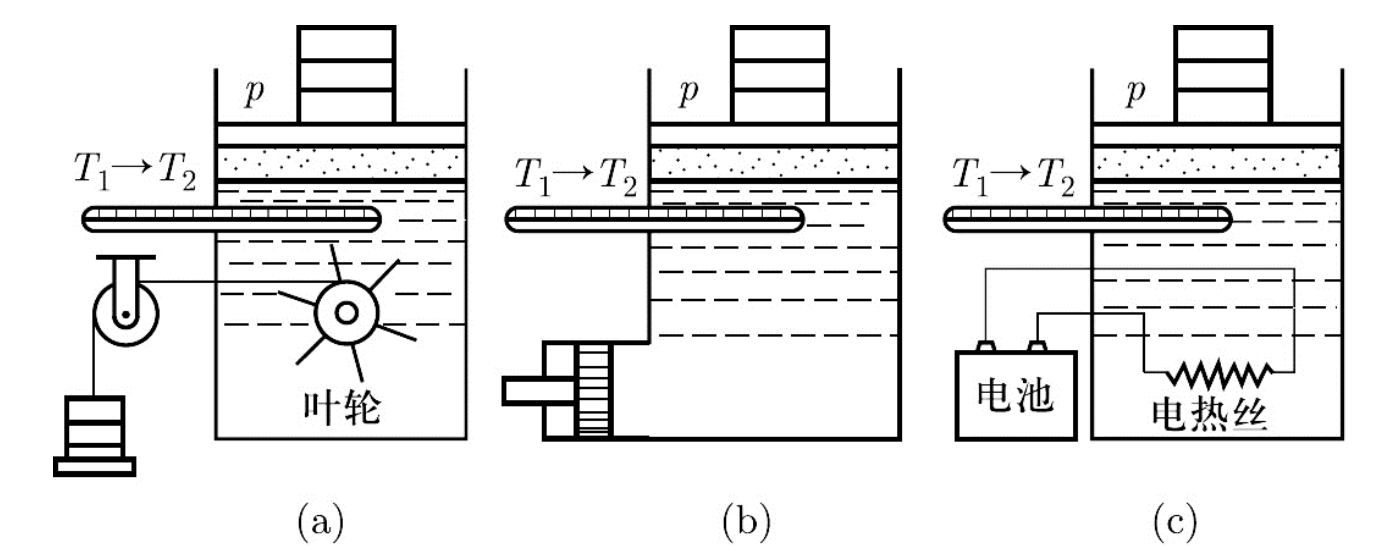
\includegraphics[width=0.7\textwidth]{joule_experiment.png}
\caption{在与外界绝热的环境内改变气体活塞系统的状态的方式（焦耳实验）（需插入原PPT第12次课第14页图片）}
\label{fig:joule_exp}
\end{figure}


\subsection{热力学第一定律在描述物体性质中的应用}

热容量：在一定的条件下，物体或系统的温度升高（降低）1K时吸收（放出）的热量。

\textbf{等体过程}：$\Delta V = 0 \implies (\Delta \boldsymbol{Q})_V = (\Delta U + p\Delta V)_V = (\Delta \boldsymbol{U})_V$

\[
\text{等体热容 }\boldsymbol{C_V} = \lim_{\Delta T \to 0}\frac{(\Delta Q)_V}{\Delta T} = \lim_{\Delta T \to 0}\frac{(\Delta U)_V}{\Delta T} = \boldsymbol{\left(\frac{\partial U}{\partial T}\right)_V}
\]

\textbf{等压过程}：$(\Delta Q)_p = (\Delta U + p\Delta V)_p = [\Delta(U+pV)]_p$

定义\textbf{焓}（Enthalpy，状态函数）$\boldsymbol{H = U + pV}$，则$(\Delta \boldsymbol{Q})_p = (\Delta \boldsymbol{H})_p$

\[
\text{等压热容 }\boldsymbol{C_p} = \lim_{\Delta T \to 0}\frac{(\Delta Q)_p}{\Delta T} = \lim_{\Delta T \to 0}\frac{(\Delta H)_p}{\Delta T} = \boldsymbol{\left(\frac{\partial H}{\partial T}\right)_p}
\]

比热容 $c_V = C_V/m$；\ $c_p = C_p/m$；\qquad 绝热指数：$\boldsymbol{\gamma = C_p/C_V}$


\subsection{内能和焓}

定义内能：$U = U_k + U_p = U(T,V)$ \qquad 焓：$H = U + pV = H(T,p)$

\[
\mathrm{d}U = \left(\frac{\partial U}{\partial T}\right)_V \mathrm{d}T + \left(\frac{\partial U}{\partial V}\right)_T \mathrm{d}V = C_V\,\mathrm{d}T + f'(T,V)\,\mathrm{d}V
\]

\[
\mathrm{d}H = \left(\frac{\partial H}{\partial T}\right)_p \mathrm{d}T + \left(\frac{\partial H}{\partial p}\right)_T \mathrm{d}p = C_p\,\mathrm{d}T + g'(T,p)\,\mathrm{d}p
\]

内能：$U(T,V) - U_0 = \displaystyle\int_{T_0}^{T} C_V\,\mathrm{d}T + f(V)$ \quad 焓：$H(T,p) - H_0 = \displaystyle\int_{T_0}^{T} C_p\,\mathrm{d}T + g(p)$

当系统温度变化时，由于体膨胀系数$\alpha \neq 0$，系统的体积都会发生变化，因此，在实验上，定体热容量很难测定，而定压热容量的测定却相对容易。那么，相对而言，系统的焓比内能容易确定。

地球表面上的物体一般都处于确定的大气压下，物态变化（或者说物相变化）及一些化学反应都在确定压强下进行，因此，在实验和工程技术中，态函数焓比内能有更重要的实用价值。


\subsection{理想气体的内能、焓及热容量}

理想气体的分子间的相互作用力可以忽略，即$U_p = \text{常量}$，则内能和热容量$C_V$都仅是温度$T$的函数。

\[
U = U(T) \implies H = U + pV = U(T) + \nu RT = H(T)
\]

\[
\boldsymbol{C_p = \left(\frac{\partial H}{\partial T}\right)_p = \left(\frac{\partial U}{\partial T}\right)_V + \nu R = C_V + \nu R} \implies \boldsymbol{C_p^{mol} - C_V^{mol} = R}
\]

绝热指数：
\[
\gamma = \frac{C_p^{mol}}{C_V^{mol}} = 1 + \frac{R}{C_V^{mol}} \implies C_V^{mol} = \frac{R}{\gamma-1};\quad C_p^{mol} = \frac{\gamma R}{\gamma-1}
\]

单原子气体：$C_V^{mol} = \dfrac{3R}{2}$；\ $C_p^{mol} = \dfrac{5R}{2}$；\ $\gamma = \dfrac{5}{3} = 1.67$

刚性双原子：$C_V^{mol} = \dfrac{5R}{2}$；\ $C_p^{mol} = \dfrac{7R}{2}$；\ $\gamma = \dfrac{7}{5} = 1.40$

\subsection{焦耳定律及其实验检验}

\textbf{焦耳定律}：理想气体的内能和焓都是态函数，且仅与温度$T$有关，与体积$V$、压强$p$无关。

实际呢？焦耳实验（绝热自由膨胀实验）

实验原理 $U = U(T,V) \implies$

\[
\Delta U = \left(\frac{\partial U}{\partial T}\right)_V \Delta T + \left(\frac{\partial U}{\partial V}\right)_T \Delta V
\]

实验中$Q = 0$；\ $W = 0 \implies \Delta U = 0$

$\Delta V \neq 0$，$\displaystyle\left(\frac{\partial U}{\partial V}\right)_T \stackrel{?}{=} 0 \iff \Delta T \stackrel{?}{=} 0$

\begin{figure}[htbp]
\centering
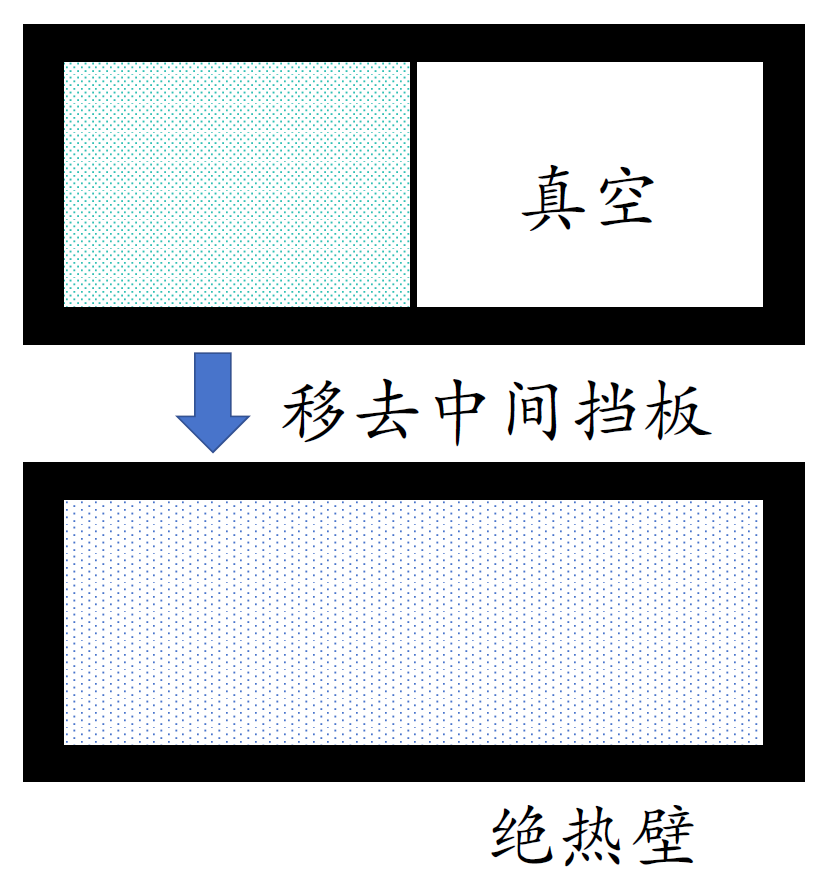
\includegraphics[width=0.4\textwidth]{fig_joule_experiment.png}
\caption{焦耳实验（绝热自由膨胀）示意图}
\label{fig:joule_experiment}
\end{figure}


% --------------------------------------------
\subsection{焦耳--汤姆逊效应}
% --------------------------------------------

\subsubsection{节流膨胀实验与等焓过程}

\paragraph{节流过程}
高压气体经过多孔塞流到低压一侧的稳定流动过程。

\paragraph{过程分析}
恒定压强差流动、绝热。
\begin{itemize}
    \item 左边：外界对系统做功 $W_1 = p_iV_i$；
    \item 右边：系统对外界做功 $W_2' = p_fV_f$；
    \item 总作功：$W = W_1 - W_2' = p_iV_i - p_fV_f$。
\end{itemize}

由热力学第一定律（绝热 $Q=0$）：
\[
\Delta U = U_f - U_i = Q + W = p_iV_i - p_fV_f
\]
整理得：
\[
U_f + p_fV_f = U_i + p_iV_i \quad\Longrightarrow\quad \boxed{H_f = H_i}
\]
即\textbf{等焓过程}。

\begin{figure}[htbp]
    \centering
    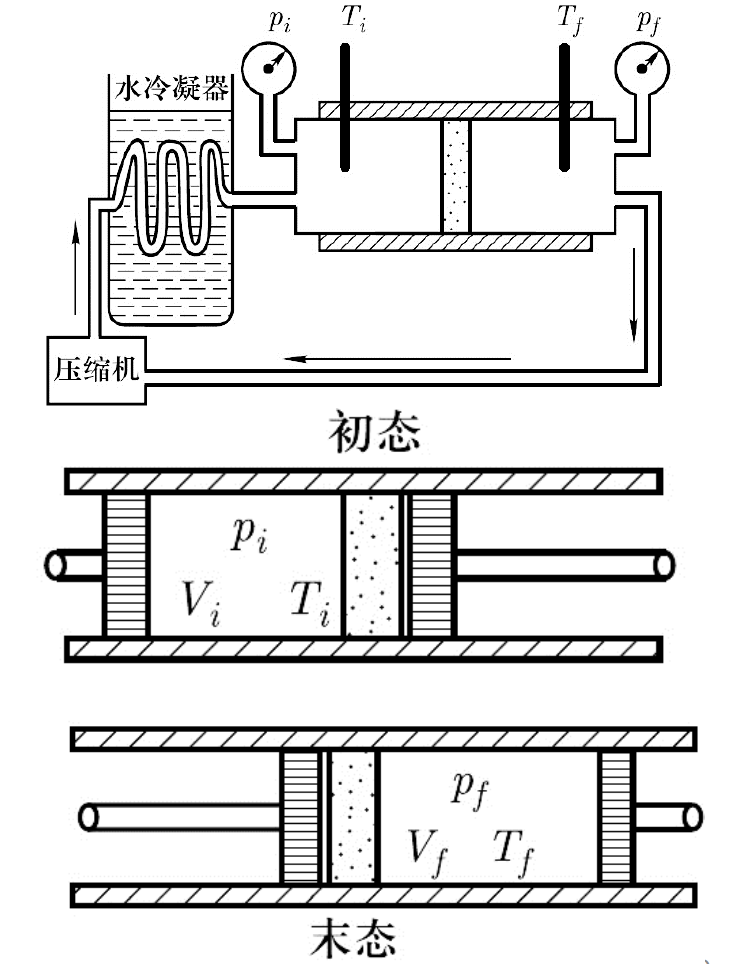
\includegraphics[width=0.5\textwidth]{JT_experiment.png}
    \caption{实验图示}
    \label{fig:JT_experiment}
\end{figure}

\subsubsection{实验结果与焦--汤效应}

\paragraph{真实气体}
实验表明，对于常温常压下节流膨胀过程：
\begin{itemize}
    \item \textbf{正效应}：通常的真实气体的温度下降（$T_f < T_i$）；
    \item \textbf{负效应}：氢、氦等气体温度上升（$T_f > T_i$）。
\end{itemize}
这种气体节流膨胀导致温度发生变化的现象称为\textbf{节流效应}，也称\textbf{焦耳--汤姆逊效应}。

\paragraph{理想气体}
理想气体的温度在节流膨胀前后保持不变，即 $T_f = T_i = \text{常量}$。代入理想气体状态方程则得 $p_iV_i = p_fV_f$。因此，理想气体系统的内能在节流膨胀过程中保持不变。这一压强、体积变化而温度不变的情况下内能不变的结果充分说明，\textbf{理想气体的内能仅是温度的函数}，从而进一步证实了\textbf{焦耳定律}。

\subsubsection{Joule--Thomson (JT) 系数与转换曲线}

\paragraph{JT 系数的定义}
焦耳--汤姆逊系数即节流过程在 $p$--$T$ 图上等焓线的斜率：
\[
\boxed{\mu = \left(\frac{\partial T}{\partial p}\right)_H}
\]
\begin{itemize}
    \item $\mu > 0$：正效应（温度下降）；
    \item $\mu < 0$：负效应（温度上升）。
\end{itemize}

\paragraph{范德瓦尔斯气体的焦--汤系数推导}

对于节流（等焓）过程：
\begin{equation}
\mathrm{d}H = \left(\frac{\partial H}{\partial T}\right)_p\mathrm{d}T + \left(\frac{\partial H}{\partial p}\right)_T\mathrm{d}p = 0
\end{equation}

由定义：
\begin{equation}
\mu = \left(\frac{\partial T}{\partial p}\right)_H = -\frac{(\partial H/\partial p)_T}{(\partial H/\partial T)_p} = \frac{-1}{C_p}\left(\frac{\partial H}{\partial p}\right)_T
\end{equation}
利用链式法则：
\begin{equation}
\mu = \frac{-1}{C_p}\left(\frac{\partial H}{\partial V_m}\right)_T\left(\frac{\partial V_m}{\partial p}\right)_T
\end{equation}

范德瓦尔斯方程：
\begin{equation}
\left(p+\frac{a}{V_m^2}\right)(V_m-b) = RT \quad\Rightarrow\quad p = \frac{RT}{V_m-b} - \frac{a}{V_m^2},\quad pV_m = \frac{RTV_m}{V_m-b} - \frac{a}{V_m}
\end{equation}

摩尔内能：
\begin{equation}
U^{mol}(T,V_m) = C_V^{mol}T - \frac{a}{V_m} + U_0 \quad (\text{动能项、势能项、参考点})
\end{equation}

摩尔焓：
\begin{equation}
H^{mol}(T,V_m) = U^{mol} + pV_m = C_V^{mol}T + \frac{RTV_m}{V_m-b} - \frac{2a}{V_m} + H_0
\end{equation}

计算 $\displaystyle\left(\frac{\partial H}{\partial V_m}\right)_T$：
\begin{equation}
\left(\frac{\partial H}{\partial V_m}\right)_T = \frac{RT(V_m-b)-RTV_m}{(V_m-b)^2} + \frac{2a}{V_m^2} = \frac{2a(V_m-b)^2-RTbV_m^2}{V_m^2(V_m-b)^2}
\end{equation}

又
\begin{equation}
\left(\frac{\partial p}{\partial V_m}\right)_T = \frac{-RT}{(V_m-b)^2} + \frac{2a}{V_m^3} = \frac{2a(V_m-b)^2-RTV_m^3}{V_m^3(V_m-b)^2}
\end{equation}
故
\begin{equation}
\left(\frac{\partial V_m}{\partial p}\right)_T = \frac{V_m^3(V_m-b)^2}{2a(V_m-b)^2-RTV_m^3} < 0
\end{equation}
（等温压缩系数 $\kappa$，得分母小于零）

于是
\begin{equation}
\left(\frac{\partial H}{\partial p}\right)_T = \frac{2a(V_m-b)^2-RTbV_m^2}{V_m^2(V_m-b)^2}\cdot\frac{V_m^3(V_m-b)^2}{2a(V_m-b)^2-RTV_m^3} = V_m\frac{2a(V_m-b)^2-RTbV_m^2}{2a(V_m-b)^2-RTV_m^3}
\end{equation}

最终得焦--汤系数：
\begin{equation}
\mu = \left(\frac{\partial T}{\partial p}\right)_H = \frac{2aV_m(V_m-b)^2-bRTV_m^3}{R^2TV_m^3+C_{V,m}\bigl[RTV_m^3-2a(V_m-b)^2\bigr]}
\end{equation}

$\mu$ 的符号取决于：\textbf{吸引势} $2aV_m(V_m-b)^2$ 和 \textbf{排斥势} $RTbV_m^3$。
\begin{itemize}
    \item $a$ 起主要作用（$r>r_0$），JT 为正；
    \item $b$ 起主要作用（$r\ll r_0$），JT 为负。
\end{itemize}

\paragraph{转换曲线}

对应于 $\mu=0$ 有 $2aV_m(V_m-b)^2 = RT_cbV_m^3$；解得
\begin{equation}
V_m = \frac{b}{1-\sqrt{\dfrac{RT_cb}{2a}}}
\end{equation}
代入 $p_c = \dfrac{RT_c}{V_m-b} - \dfrac{a}{V_m^2}$ 并化简：
\begin{equation}
p_c = \frac{a}{b^2}\left(1-\sqrt{\frac{RT_cb}{2a}}\right)\left(3\sqrt{\frac{RT_cb}{2a}}-1\right)
\end{equation}

$p_c=0$ 时：
\begin{equation}
T_c^u = \frac{2a}{Rb},\quad T_c^d = \frac{2a}{9Rb}
\end{equation}
$\dfrac{\partial p_c}{\partial T_c}=0$ 时：
\begin{equation}
p_{c0} = \frac{a}{3b^2},\quad T_{c0} = \frac{8a}{9Rb}
\end{equation}

\paragraph{常见气体的最高上转换温度}
\begin{center}
\begin{tabular}{c|c}
\hline
气体 & 最高上转换温度 \\
\hline
He & $\sim 40\ \mathrm{K}$ \\
H$_2$ & $202\ \mathrm{K}$ \\
Ne & $231\ \mathrm{K}$ \\
N$_2$ & $621\ \mathrm{K}$ \\
Air & $659\ \mathrm{K}$ \\
O$_2$ & $764\ \mathrm{K}$ \\
Ar & $780\ \mathrm{K}$ \\
CO$_2$ & $\sim 1500\ \mathrm{K}$ \\
\hline
\end{tabular}
\end{center}

\paragraph{微观定性解释}
气体存在相互作用势能：
\begin{itemize}
    \item \textbf{吸引势主导}：$p\downarrow \Rightarrow V\uparrow \Rightarrow U_p\uparrow \Rightarrow U_k\downarrow \Rightarrow T\downarrow \Rightarrow \mu > 0$；
    \item \textbf{排斥势主导}：$p\downarrow \Rightarrow V\uparrow \Rightarrow U_p\downarrow \Rightarrow U_k\uparrow \Rightarrow T\uparrow \Rightarrow \mu < 0$。
\end{itemize}

\begin{figure}[htbp]
    \centering
    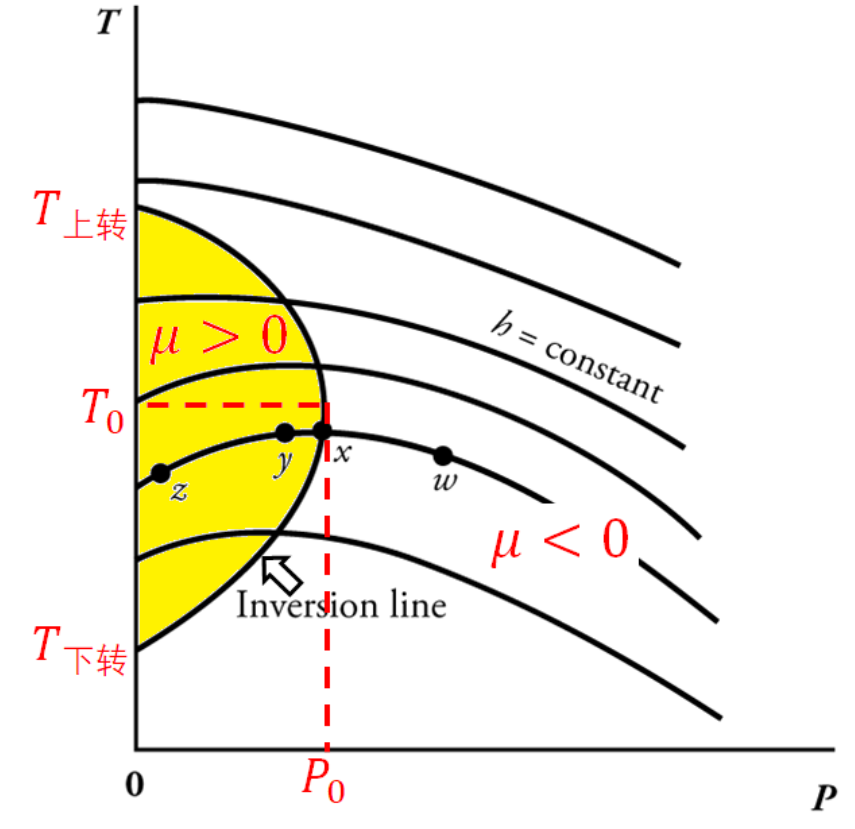
\includegraphics[width=0.5\textwidth]{JT_curve.png}
    \caption{转换曲线}
    \label{fig:JT_curve}
\end{figure}

\subsubsection*{应用举例——气体液化}

低温工程中常用节流膨胀效应使气体降温和液化。

利用该方法，林德（C. von Linde）和汉普森（W. Hampson）于1895年实现了对空气的液化。

\textbf{优点}：随着温度降低，焦耳—汤姆孙系数增大，即温度越低降温效率越高。

\textbf{缺点}：只有在一定的温度之下才具有焦耳—汤姆孙正效应，通常需要先采用其它方法进行预冷。

\begin{figure}[htbp]
\centering
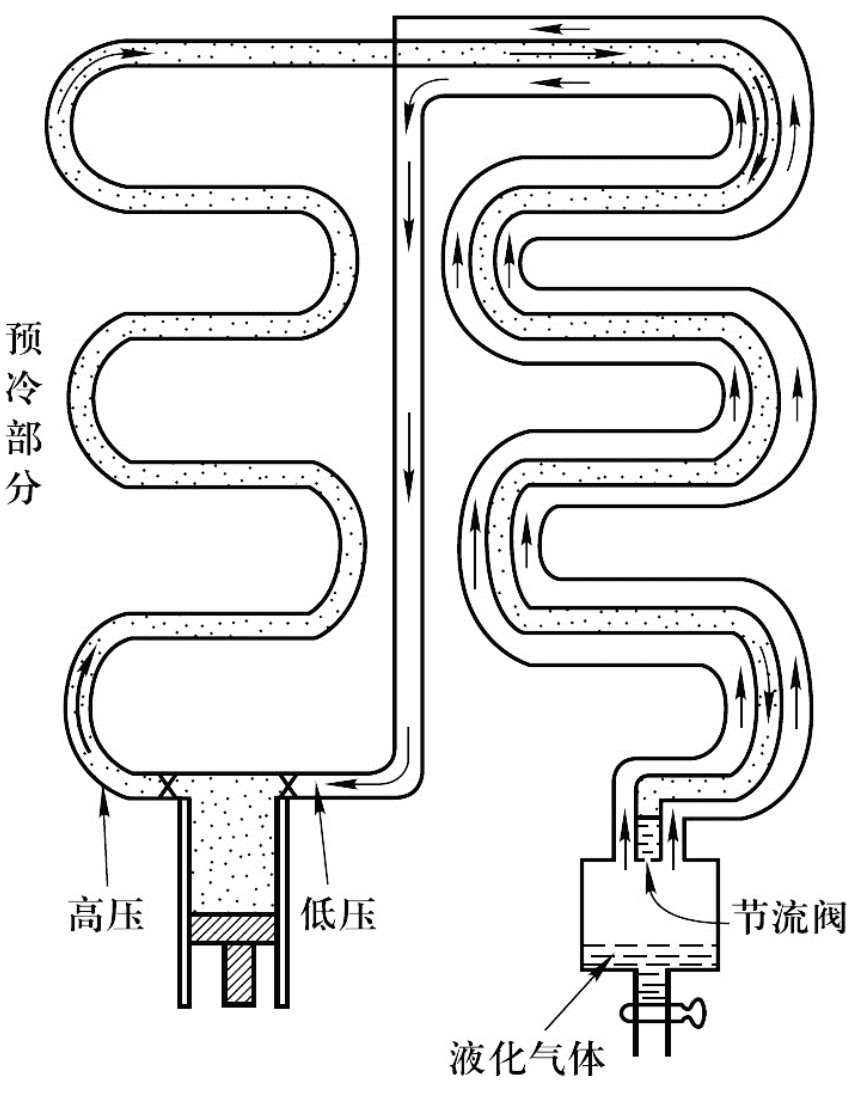
\includegraphics[width=0.3\textwidth]{gas_liquefaction.png}
\caption{利用节流膨胀效应液化气体的装置示意图（需插入原PPT第13次课第5页图片）}
\label{fig:liquefaction}
\end{figure}

% --------------------------------------------
\subsection{热力学第一定律对理想气体的应用}
% --------------------------------------------

\subsubsection*{等体过程}

$V = \text{常量}$，或 $\dfrac{T}{p} = \text{常量}$。
\begin{align}
\Delta V &= 0 \Rightarrow W = 0 \Rightarrow \Delta U = Q \\
\mathrm{d}Q &= \mathrm{d}U = \left(\frac{\partial U}{\partial T}\right)_V\mathrm{d}T = C_V\mathrm{d}T \\
\Delta U &= \int_{T_1}^{T_2} C_V\,\mathrm{d}T = C_V\Delta T
\end{align}

\subsubsection*{等压过程}

$p = \text{常量}$，或 $\dfrac{T}{V} = \text{常量}$。
\begin{align}
\mathrm{d}W &= -p\,\mathrm{d}V,\quad W = -\int_{V_1}^{V_2}p\,\mathrm{d}V = -p(V_2-V_1) \\
\mathrm{d}Q_p &= C_p\,\mathrm{d}T,\quad Q_p(1\to 2) = \int_{T_1}^{T_2}C_p\,\mathrm{d}T = C_p\Delta T \\
\Delta U &= Q+W = C_p\Delta T - p(V_2-V_1) = (C_p-\nu R)\Delta T = C_V\Delta T \\
Q &= \Delta U - W = U_2-U_1+p(V_2-V_1) = H_2-H_1 = \Delta H
\end{align}

\textbf{等压过程中系统焓的增加量等于系统从外界吸收的热量。}

\subsubsection*{等温过程}

$T = \text{常量} \Rightarrow pV = \text{常量}$。
\begin{align}
U &= U(T) \Rightarrow \Delta U = 0 \\
Q &= -W = \int_{V_1}^{V_2}p\,\mathrm{d}V = \frac{m}{M}RT\int_{V_1}^{V_2}\frac{1}{V}\,\mathrm{d}V = \frac{m}{M}RT\ln\frac{V_2}{V_1}
\end{align}

\textbf{等温膨胀过程中，理想气体系统对外界所作的功全部来源于系统从外界吸收的热量。}

\subsubsection*{绝热过程}

$Q=0$。
\begin{align}
\mathrm{d}U &= C_V\mathrm{d}T = \mathrm{d}W = -p\,\mathrm{d}V = -\frac{m}{M}RT\frac{\mathrm{d}V}{V} \\
C_V\frac{\mathrm{d}T}{T} &= -\frac{m}{M}R\frac{\mathrm{d}V}{V} = -(C_p-C_V)\frac{\mathrm{d}V}{V} \\
\mathrm{d}\bigl(\ln T + (\gamma-1)\ln V\bigr) &= 0
\end{align}

积分得绝热过程方程：
\begin{equation}
\boxed{TV^{\gamma-1} = \text{常量},\quad pV^\gamma = \text{常量},\quad \frac{p^{\gamma-1}}{T^\gamma} = \text{常量}}
\end{equation}

其中
\begin{equation}
\boxed{C_p^{mol}-C_V^{mol}=R,\quad \gamma=\frac{C_p^{mol}}{C_V^{mol}}=1+\frac{R}{C_V^{mol}}}
\end{equation}

$p$-$V$ 图上连接绝热过程初末态点的曲线较等温线陡。

\begin{figure}[htbp]
\centering
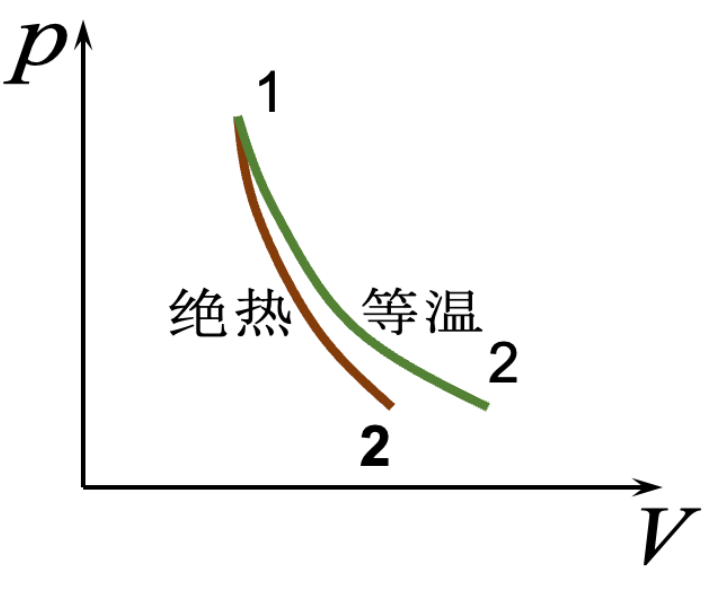
\includegraphics[width=0.35\textwidth]{adiabatic.png}
\caption{绝热过程与等温过程 $p$-$V$ 图对比（需插入原PPT第13次课第9页示意图）}
\label{fig:adiabatic}
\end{figure}

\subsubsection*{绝热过程做功}

系统对外做功 $W' = -W$：
\begin{equation}
W' = \int_{V_1}^{V_2}p\,\mathrm{d}V = p_1V_1^\gamma\int_{V_1}^{V_2}\frac{\mathrm{d}V}{V^\gamma} = p_1V_1^\gamma\frac{V_1^{1-\gamma}-V_2^{1-\gamma}}{\gamma-1} = \frac{p_1V_1-p_2V_2}{\gamma-1}
\end{equation}

利用 $pV=\nu RT$ 和 $C_p-C_V=\nu R$，有
\begin{equation}
\frac{p_iV_i}{\gamma-1} = \frac{\nu RT_i}{\dfrac{C_p}{C_V}-1} = \frac{C_V\nu RT_i}{C_p-C_V} = \frac{C_V\nu RT_i}{\nu R} = C_VT_i
\end{equation}

故\textbf{绝热过程做功等于内能改变量}：
\begin{equation}
\boxed{W = C_V(T_2-T_1)}
\end{equation}

\subsubsection*{讨论：非准静态过程与自由膨胀}

以上所有过程都是在\textbf{准静态假设}下的推理。对于一个\textbf{非准静态过程}，上面的公式\textbf{不能直接应用}。但\textbf{状态函数与过程无关}，可以用来计算非准静态过程。

\textbf{讨论 1 mol 理想气体自由膨胀的过程：$V_f=2V_0$}

向真空自由膨胀过程中既不传热（$\Delta Q=0$）又不作功（$\Delta W=0$），真空自由膨胀过程是\textbf{绝热的}（$\Delta Q=0$），也是\textbf{等温的}（$\Delta U=0,\ \Delta T=0$）。但是，由于其进行得太快，\textbf{不是准静态过程}。

自由膨胀过程 $Q=W=0$，$T_f=T_0$，故
\begin{equation}
U_f=U_0,\quad H_f=H_0,\quad p_f=\frac{p_0}{2},\quad V_f=2V_0
\end{equation}

等温过程 $T_f=T_0$，$pV=\text{常量}$，末态同样有
\begin{equation}
U_f=U_0,\quad H_f=H_0,\quad p_f=\frac{p_0}{2},\quad V_f=2V_0
\end{equation}

\textbf{相同初态经等温过程达到的末态与经自由膨胀过程达到的末态相同，但做功/吸热不同}：
\begin{equation}
Q = -W = \int_{V_1}^{V_2}p\,\mathrm{d}V = RT\int_{V_1}^{V_2}\frac{\mathrm{d}V}{V} = RT\ln\frac{V_2}{V_1} = RT\ln 2 \neq 0
\end{equation}

绝热过程（$A\Rightarrow C$）$pV^\gamma=\text{const}$：
\begin{align}
p_f &= \frac{p_0V_0^\gamma}{V_f^\gamma} = \frac{p_0V_0^\gamma}{(2V_0)^\gamma} = \frac{p_0}{2^\gamma} < \frac{p_0}{2}\quad (\gamma>1) \\
T_f &= \frac{T_0V_0^{\gamma-1}}{V_f^{\gamma-1}} = \frac{T_0V_0^{\gamma-1}}{(2V_0)^{\gamma-1}} = \frac{T_0}{2^{\gamma-1}} < T_0
\end{align}

绝热过程做功：
\begin{equation}
W_{ad} = \Delta U_{ad} = C_V(T_f-T_0) = C_VT_0\left(\frac{1}{2^{\gamma-1}}-1\right) < 0
\end{equation}

\textbf{相同的初态（A）经绝热过程达到的末态（C）与经自由膨胀过程达到的末态（B）不相同}。

为使绝热过程后达到的末态与经自由膨胀达到的末态相同，需要一个等体加热过程 $C\to B$。该等体过程中：
\begin{align}
Q_{ic} &= C_V(T_f-T_i) = C_V\left(T_0-\frac{T_0}{2^{\gamma-1}}\right) > 0 \\
W_{ic} &= 0,\quad \Delta U_{ic} = Q_{ic}+W_{ic} = C_V\left(T_0-\frac{T_0}{2^{\gamma-1}}\right) > 0
\end{align}

联合过程：
\begin{equation}
W_{ad+ic} = C_VT_0\left(\frac{1}{2^{\gamma-1}}-1\right) < 0,\quad \Delta U_{ad+ic} = Q_{ad+ic}+W_{ad+ic} = 0
\end{equation}

\begin{figure}[htbp]
\centering
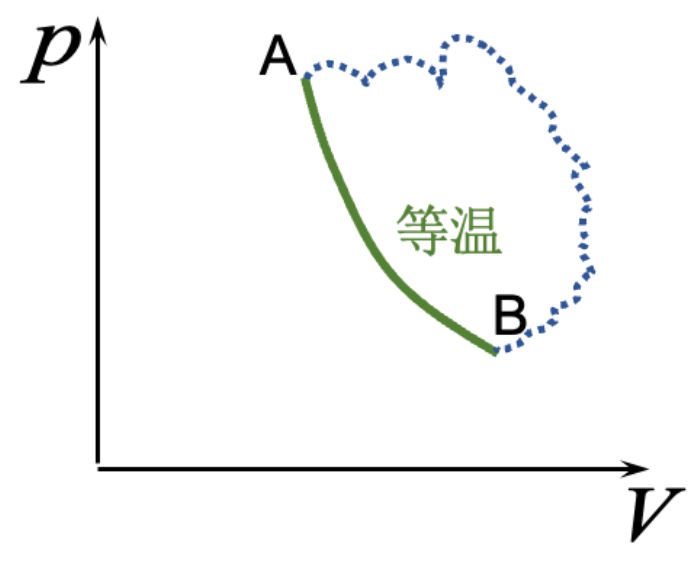
\includegraphics[width=0.5\textwidth]{free_expansion.png}
\caption{自由膨胀、等温与绝热过程末态对比（需插入原PPT第13次课第12--14页示意图）}
\label{fig:freeexpansion}
\end{figure}

% --------------------------------------------
\subsection{大气层的压力与温度随高度的变化}
% --------------------------------------------

\subsubsection*{等温大气模型}

\begin{equation}
p = p_0\exp\!\left(-\frac{mgz}{k_BT}\right)
\end{equation}

\subsubsection*{绝热大气模型}

实际对流气体上升缓慢，过程可视为\textbf{准静态}的；干燥空气导热性能很差，过程又可视为\textbf{绝热}的；所以干燥大气的温度垂直分布可用\textbf{准静态绝热过程}模型描述：
\begin{equation}
pV^\gamma = p_0V_0^\gamma,\quad V=\frac{\nu RT}{p} \Rightarrow p^{1-\gamma}T^\gamma = p_0^{1-\gamma}T_0^\gamma
\end{equation}

求全微分：
\begin{equation}
(1-\gamma)p^{-\gamma}T^\gamma\,\mathrm{d}p + \gamma p^{1-\gamma}T^{\gamma-1}\,\mathrm{d}T = 0 \Rightarrow (1-\gamma)\frac{\mathrm{d}p}{p} + \gamma\frac{\mathrm{d}T}{T} = 0
\end{equation}

\subsubsection*{干绝热递减率（DALR）}

\begin{equation}
\frac{\mathrm{d}T}{T} = \frac{\gamma-1}{\gamma}\frac{\mathrm{d}p}{p} = -\frac{\gamma-1}{\gamma}\frac{Mg}{RT}\,\mathrm{d}z
\end{equation}

积分得线性关系：
\begin{equation}
T(z) = T_0\left[1-\left(\frac{Mg}{RT_0}\frac{\gamma-1}{\gamma}\right)z\right]
\end{equation}

压强随高度变化：
\begin{equation}
p = p_0\left(\frac{T}{T_0}\right)^{\frac{\gamma}{\gamma-1}} \Rightarrow p(z) = p_0\left[1-\left(\frac{Mg}{RT_0}\frac{\gamma-1}{\gamma}\right)z\right]^{\frac{\gamma}{\gamma-1}}
\end{equation}

温度梯度：
\begin{equation}
\frac{\mathrm{d}T}{\mathrm{d}z} = -\frac{Mg}{R}\frac{\gamma-1}{\gamma} \approx -9.8\,\frac{\mathrm{K}}{\mathrm{km}} \approx -10\,\frac{\mathrm{K}}{\mathrm{km}}
\end{equation}

当 $\gamma\to 1$ 时，回到等温压强公式 $p=p_0\exp[-mgz/(k_BT)]$。

\subsubsection*{饱和绝热递减率（SALR）}

前面讨论的是理想气体，如果有水的相变？$\Delta U = Q + W$。

考虑1摩尔气体，气体体积为 $V$；其中水蒸气摩尔百分比，即有水蒸气 $\nu_w$ 摩尔；水蒸气摩尔汽化热 $\Lambda^{mol}$。

\begin{align}
C_V^{mol}\mathrm{d}T &= -\Lambda^{mol}\,\mathrm{d}\nu_w - p\,\mathrm{d}V,\quad \mathrm{d}(pV)=p\,\mathrm{d}V+V\,\mathrm{d}p=R\,\mathrm{d}T \\
\Rightarrow C_V^{mol}\mathrm{d}T &= -\Lambda^{mol}\,\mathrm{d}\nu_w - R\,\mathrm{d}T + V\,\mathrm{d}p \\
\Rightarrow C_p^{mol}\mathrm{d}T &= -\Lambda^{mol}\,\mathrm{d}\nu_w + RT\frac{\mathrm{d}p}{p}
\end{align}

利用 $\dfrac{\mathrm{d}p}{p}=-\dfrac{Mg}{RT}\,\mathrm{d}z$，得
\begin{equation}
\mathrm{d}T = \frac{R}{C_p^{mol}}\left(T\frac{\mathrm{d}p}{p}-\frac{\Lambda^{mol}\,\mathrm{d}\nu_w}{R}\right) = -\frac{\gamma-1}{\gamma}\left(\frac{Mg}{R}\,\mathrm{d}z + \frac{\Lambda^{mol}\,\mathrm{d}\nu_w}{R}\right)
\end{equation}

于是
\begin{align}
\frac{\mathrm{d}T}{\mathrm{d}z} &= \boxed{-\frac{\gamma-1}{\gamma}\left(\frac{Mg}{R}+\frac{\Lambda^{mol}}{R}\frac{\mathrm{d}\nu_w}{\mathrm{d}z}\right)} \quad \text{(SALR)} \\[6pt]
\frac{\mathrm{d}T}{\mathrm{d}z} &= \boxed{-\frac{\gamma-1}{\gamma}\frac{Mg}{R}} \quad \text{(DALR)}
\end{align}

由于 $\dfrac{\mathrm{d}\nu_w}{\mathrm{d}z}<0$（水蒸气含量随高度降低），故
\begin{equation}
\boxed{|\text{SALR}| < |\text{DALR}|}
\end{equation}

\subsubsection*{焚风（干热风）}

\begin{figure}[htbp]
\centering
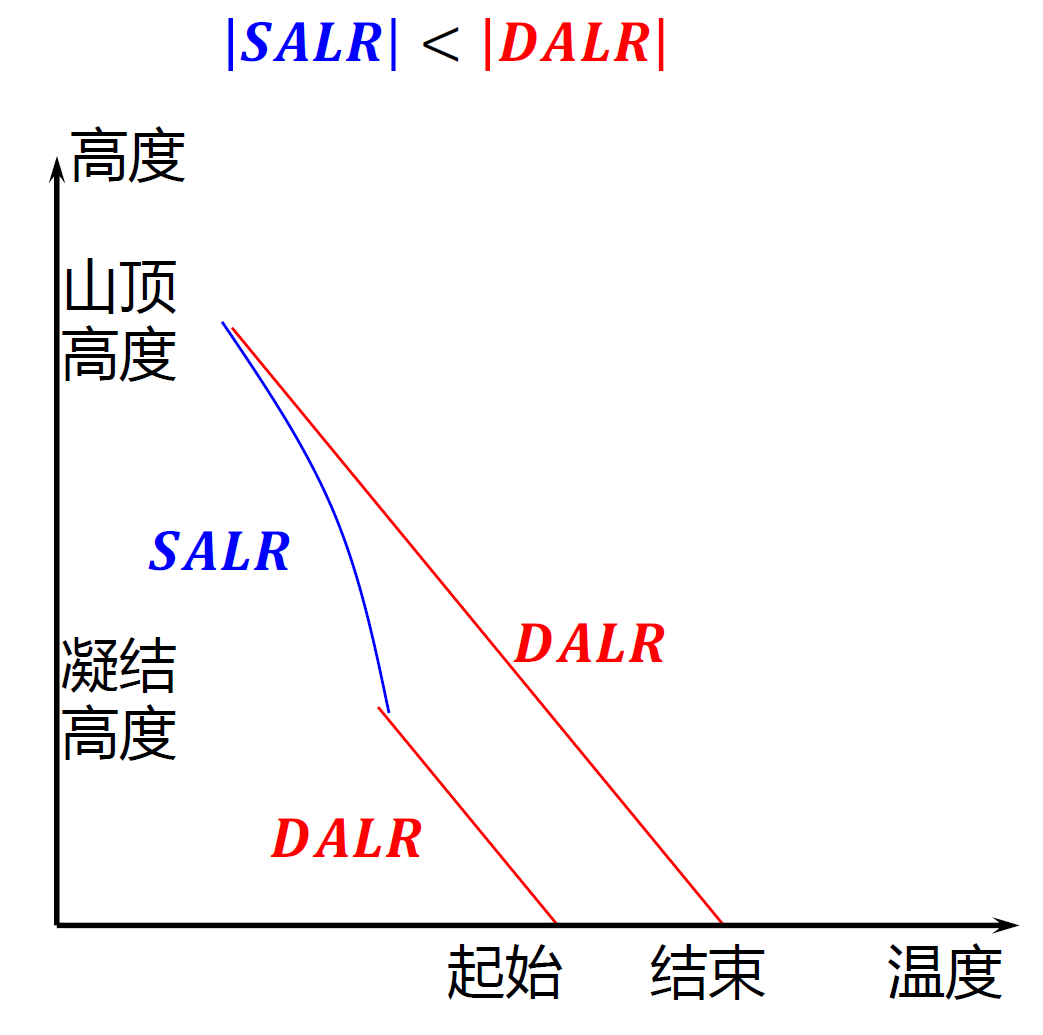
\includegraphics[width=0.45\textwidth]{foehn_diagram.png}
\caption{焚风形成示意图（需插入原PPT第14次课第6页或第7页图片）}
\label{fig:foehn}
\end{figure}

% --------------------------------------------
\subsection{多方过程}
% --------------------------------------------

前面几种准静态过程可以概括为：
\begin{equation}
pV^n = \text{常数}
\end{equation}

\begin{itemize}
    \item 等压：$n=0$
    \item 等温：$n=1$
    \item 绝热：$n=\gamma$
    \item 等体：$n\to\infty$
\end{itemize}

\textbf{多方过程}：$pV^n=\text{常数}$，多方指数 $n\neq 0,1,\gamma,\infty$。

等价形式：
\begin{equation}
TV^{n-1} = \text{常数},\quad \frac{p^{n-1}}{T^n} = \text{常数}
\end{equation}

\textbf{做功}：
\begin{equation}
W = \frac{p_2V_2-p_1V_1}{n-1} = \frac{\nu R}{n-1}(T_2-T_1)
\end{equation}

\textbf{内能}：
\begin{equation}
\Delta U = C_V(T_2-T_1)
\end{equation}

\textbf{传热}：
\begin{equation}
Q = C_n(T_2-T_1) = \Delta U - W
\end{equation}

\textbf{热容}：
\begin{equation}
\boxed{C_n = C_V - \frac{\nu R}{n-1} = \frac{nC_V-(C_V+\nu R)}{n-1} = \frac{nC_V-C_p}{n-1} = \left(\frac{n-\gamma}{n-1}\right)C_V}
\end{equation}

\begin{figure}[htbp]
\centering
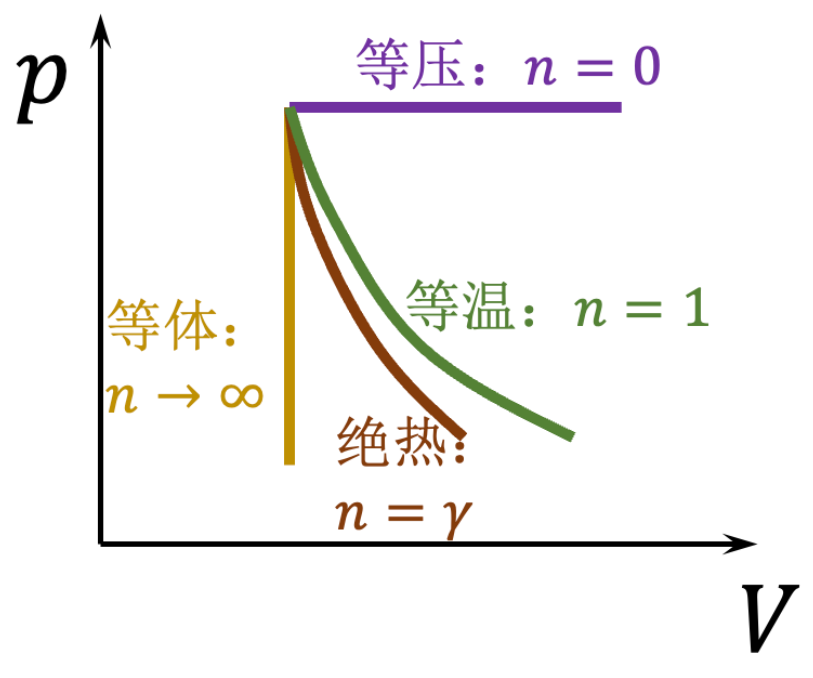
\includegraphics[width=0.45\textwidth]{polytropic_process.png}
\caption{多方过程在 $p$-$V$ 图上的表示（需插入原PPT第14次课第10页图片）}
\label{fig:polytropic}
\end{figure}

\subsubsection*{多方过程的热容与负热容}

由 $C_n = \left(\dfrac{n-\gamma}{n-1}\right)C_V$ 可知：

当 $1<n<\gamma$ 时，\textbf{热容为负}。

\begin{remark}
根据热力学第一定律 $\Delta U = \Delta Q + W$：
\begin{itemize}
    \item 如果 $\Delta Q>0,\ W<<0$，但 $|W|>\Delta Q$，则 $\Delta U<<0$，从而 $\Delta T<<0$；
    \item 如果 $\Delta Q<<0,\ W>0$，且 $W>|\Delta Q|$，则 $\Delta U>0$，从而 $\Delta T>0$。
\end{itemize}
这正是负热容的物理含义：系统吸热反而降温，或放热反而升温，因为外界对系统做的功（或系统对外做的功）的绝对值超过了传热。
\end{remark}

\begin{figure}[htbp]
\centering
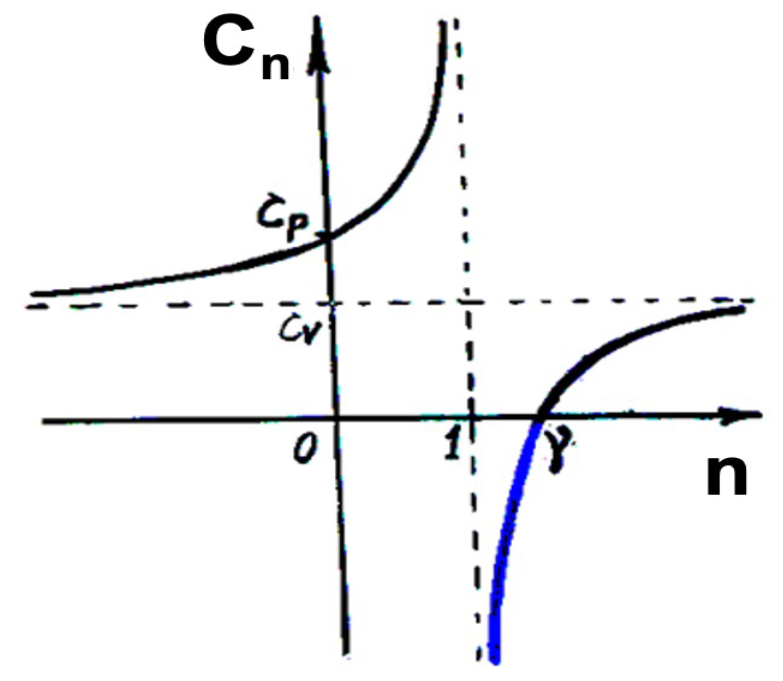
\includegraphics[width=0.45\textwidth]{cn_curve.png}
\caption{$C_n$-$n$ 曲线（需插入原PPT第14次课第11页图片）}
\label{fig:cncurve}
\end{figure}

\subsubsection*{例题：理想气体吸放热}

\textbf{题目}：$1\,\mathrm{mol}$ 单原子分子理想气体经历如图所示过程 $ab$（直线段），讨论由 $a$ 到 $b$ 的过程中系统吸放热情况。

\textbf{已知}（由图读取）：
\begin{align*}
a\text{点}&:\ p_a=15\times 10^4\,\mathrm{Pa},\quad V_a=1\times 10^{-3}\,\mathrm{m}^3 \\
b\text{点}&:\ p_b=5\times 10^4\,\mathrm{Pa},\quad V_b=3\times 10^{-3}\,\mathrm{m}^3
\end{align*}

\textbf{解}：$a$ 到 $b$ 的过程方程为直线：
\begin{equation}
p = KV + C
\end{equation}

由状态方程 $T=\dfrac{pV}{R}=\dfrac{KV^2+CV}{R}$。

元功：
\begin{equation}
\mathrm{d}W = -p\,\mathrm{d}V = -(KV+C)\,\mathrm{d}V
\end{equation}

内能变化（单原子 $C_V=\dfrac{3}{2}R$）：
\begin{equation}
\mathrm{d}U = C_V\,\mathrm{d}T = \frac{3}{2}R\cdot\frac{2KV+C}{R}\,\mathrm{d}V = (3KV+1.5C)\,\mathrm{d}V
\end{equation}

由第一定律 $\mathrm{d}Q = \mathrm{d}U-\mathrm{d}W$：
\begin{equation}
\mathrm{d}Q = (3KV+1.5C)\,\mathrm{d}V + (KV+C)\,\mathrm{d}V = (4KV+2.5C)\,\mathrm{d}V
\end{equation}

设在 $e$ 点 $Q$ 的变化率为零，即 $\mathrm{d}Q=0$：
\begin{equation}
4KV_e+2.5C = 0 \Rightarrow V_e = -\frac{2.5C}{4K}
\end{equation}

代入具体数据：
\begin{align*}
K &= -5\times 10^7\,\mathrm{Pa/m^3} \\
C &= 2\times 10^5\,\mathrm{Pa} \\
V_e &= 2.5\times 10^{-3}\,\mathrm{m^3}
\end{align*}

\textbf{结论}：系统在 $a\to e$ 段吸热，在 $e\to b$ 段放热。

代入数据积分得：
\begin{equation}
\boxed{Q_{a\to e} = 225\,\mathrm{J},\quad Q_{e\to b} = -25\,\mathrm{J}}
\end{equation}

\begin{figure}[htbp]
\centering
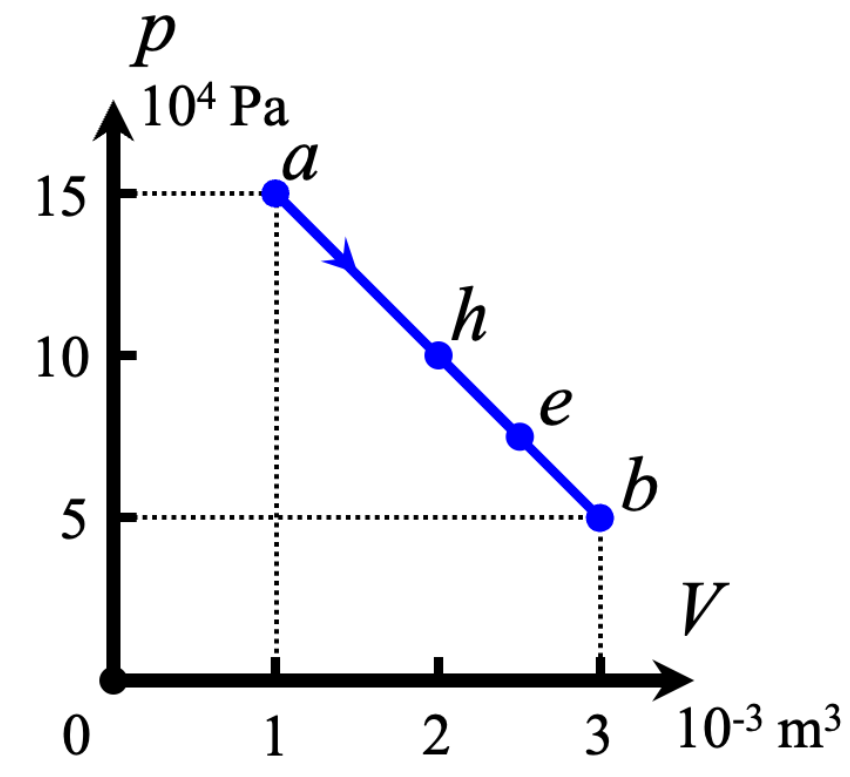
\includegraphics[width=0.35\textwidth]{heat_absorption_pv.png}
\caption{理想气体直线过程吸放热分析（需插入原PPT第14次课第12--13页图片）}
\label{fig:heat absorption}
\end{figure}

% --------------------------------------------
\subsection{循环过程与卡诺循环}
% --------------------------------------------

\subsubsection*{蒸汽机的历史（简略）}

\begin{itemize}
    \item Aeolipile（汽转球）：公元1世纪，古希腊，Heron of Alexandria
    \item 蒸汽泵：1698，英国，Thomas Savery
    \item 纽科门蒸汽机：1712，英国，Thomas Newcomen
\end{itemize}

\subsubsection*{循环过程}

系统由某一状态出发，经过任意的一系列过程，最后回到原来的状态，称为\textbf{循环过程}。对于无外场的系统，若循环过程是准静态的，则可在 $p$-$V$ 图上表示为一条闭合曲线。

\textbf{符号约定}：在 $p$-$V$ 图上，顺时针方向的循环称为\textbf{正循环}，逆时针方向的循环称为\textbf{逆循环}。

循环过程的基本性质：由于内能是状态函数，经过一个循环后系统回到初态，故
\begin{equation}
\Delta U = 0.
\end{equation}
由热力学第一定律 $\Delta U = Q - W'$（其中 $W'$ 为系统对外界所作的功），可得
\begin{equation}
Q = W'.
\end{equation}

\begin{itemize}
\item \textbf{正循环}：$W' = Q > 0$，系统从外界吸热并对外作功，对应\textbf{热机}；
\item \textbf{逆循环}：$W' = Q < 0$，外界对系统作功并向外界放热，对应\textbf{制冷机}或\textbf{热泵}。
\end{itemize}

\subsubsection*{热机效率}

正循环过程中，热机从高温热源（温度为 $T_1$）吸收热量 $Q_1$，对外作功 $W'$，同时向低温热源（温度为 $T_2$）放出热量 $Q_2'$。由能量守恒
\begin{equation}
W' = Q_1 - Q_2'.
\end{equation}

\textbf{热机效率}（循环效率）定义为系统对外所作的功与从高温热源吸收的热量之比：
\begin{equation}
\boxed{\eta = \frac{W'}{Q_1} = \frac{Q_1 - Q_2'}{Q_1} = 1 - \frac{Q_2'}{Q_1}}.
\end{equation}

\subsubsection*{制冷系数}

逆循环过程中，外界对系统作功 $W$，系统从低温热源（温度为 $T_2$）吸收热量 $Q_2$，向高温热源（温度为 $T_1$）放出热量 $Q_1'$。由能量守恒
\begin{equation}
Q_1' = Q_2 + W.
\end{equation}

\textbf{制冷系数}定义为从低温热源吸收的热量与外界对系统所作的功之比：
\begin{equation}
\boxed{\varepsilon = \frac{Q_2}{W} = \frac{Q_2}{Q_1' - Q_2}}.
\end{equation}

\subsubsection*{卡诺循环}

\textbf{卡诺循环}是由两个等温过程和两个绝热过程组成的理想准静态循环。工作物质为理想气体时，其在 $p$-$V$ 图上的表示如图所示：

\begin{figure}[htbp]
\centering
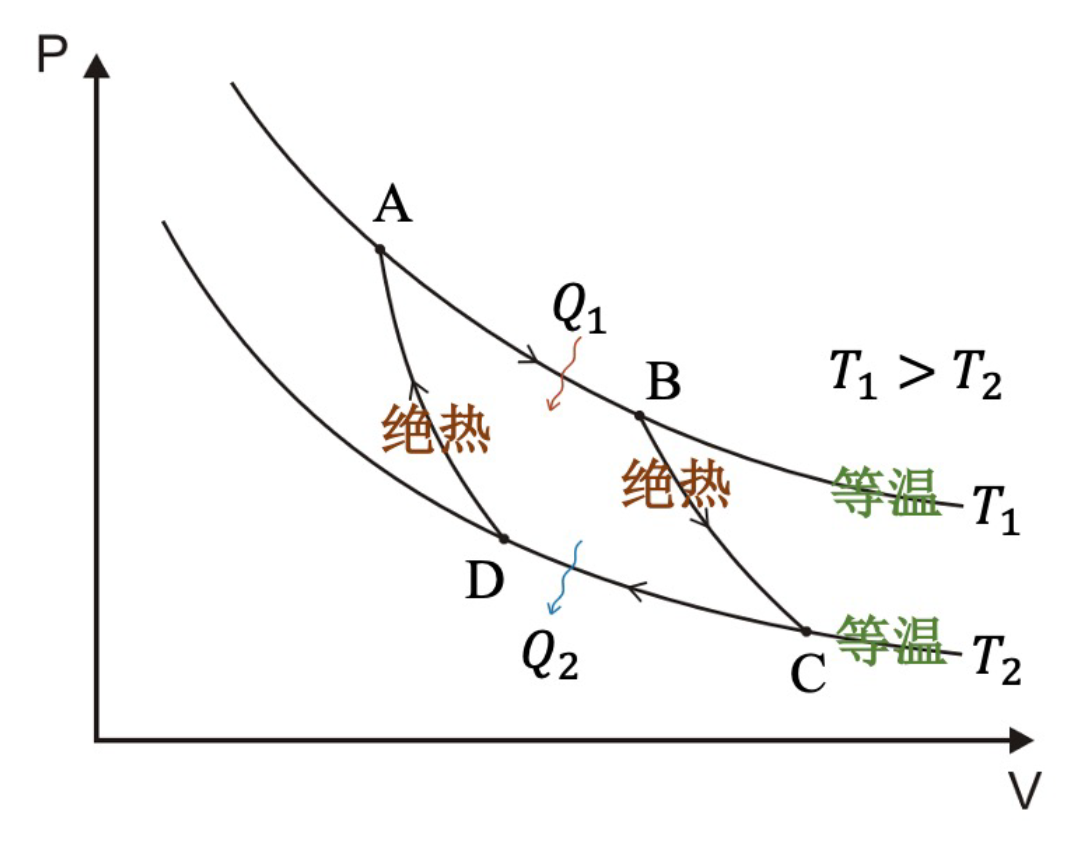
\includegraphics[width=0.35\textwidth]{carnot_cycle_pv.png}
\caption{理想气体卡诺循环在 $p$-$V$ 图上的表示（需插入原PPT图片）}
\label{fig:carnot_cycle}
\end{figure}

各过程的特征如下：
\begin{itemize}
\item \textbf{AB（等温膨胀）}：系统与高温热源 $T_1$ 接触，吸热 $Q_1$，对外作功；
\item \textbf{BC（绝热膨胀）}：系统脱离热源，对外作功，温度由 $T_1$ 降至 $T_2$；
\item \textbf{CD（等温压缩）}：系统与低温热源 $T_2$ 接触，放热 $Q_2'$，外界对系统作功；
\item \textbf{DA（绝热压缩）}：系统脱离冷源，外界对系统作功，温度由 $T_2$ 升至 $T_1$。
\end{itemize}

\subsubsection*{理想气体卡诺循环的效率}

对理想气体的可逆卡诺正循环，各过程的热量与功计算如下：

\textbf{吸热}（AB 等温膨胀，$T=T_1$）：
\begin{equation}
Q_1 = \nu RT_1\ln\frac{V_B}{V_A}.
\end{equation}

\textbf{放热}（CD 等温压缩，$T=T_2$）：
\begin{equation}
Q_2' = \nu RT_2\ln\frac{V_C}{V_D}.
\end{equation}

于是热机效率
\begin{equation}
\eta = \frac{W'}{Q_1} = \frac{Q_1 - Q_2'}{Q_1}
= \frac{\nu RT_1\ln\dfrac{V_B}{V_A} - \nu RT_2\ln\dfrac{V_C}{V_D}}{\nu RT_1\ln\dfrac{V_B}{V_A}}.
\end{equation}

利用绝热过程方程 $TV^{\gamma-1}=\text{const}$，对 BC 和 DA 两段绝热过程有
\begin{equation}
T_1 V_B^{\gamma-1} = T_2 V_C^{\gamma-1},\qquad
T_1 V_A^{\gamma-1} = T_2 V_D^{\gamma-1}.
\end{equation}
两式相除得
\begin{equation}
\frac{V_B}{V_A} = \frac{V_C}{V_D}.
\end{equation}

代入效率表达式，化简得
\begin{equation}
\boxed{\eta = 1 - \frac{T_2}{T_1} = \frac{T_1 - T_2}{T_1}}.
\end{equation}

\begin{remark}
卡诺循环的效率只与两个热源的热力学温度有关，与工作物质无关，且是所有工作于相同热源之间的热机中效率最高的。
\end{remark}

\subsubsection*{理想气体逆卡诺循环的制冷系数}

对逆卡诺循环，系统从低温热源 $T_2$ 吸热 $Q_2$，向高温热源 $T_1$ 放热 $Q_1'$，外界对系统作功 $W$。类似地有
\begin{equation}
Q_2 = \nu RT_2\ln\frac{V_C}{V_D},\qquad
Q_1' = \nu RT_1\ln\frac{V_B}{V_A}.
\end{equation}
利用同样的绝热关系 $\dfrac{V_B}{V_A}=\dfrac{V_C}{V_D}$，可得制冷系数
\begin{equation}
\boxed{\varepsilon = \frac{Q_2}{W} = \frac{Q_2}{Q_1'-Q_2} = \frac{T_2}{T_1-T_2}}.
\end{equation}

\subsubsection*{几种常见的热力学循环}

除卡诺循环外，工程上还有几种重要的循环：

\begin{itemize}
\item \textbf{奥托循环（Otto cycle）}：等体加热循环，由两个绝热过程和两个等体过程组成。\\
压缩比 $r=\dfrac{V_1}{V_2}$，效率为
\begin{equation}
\boxed{\eta_{\text{奥托}} = 1 - \frac{1}{r^{\gamma-1}}}.
\end{equation}
应用于四冲程火花点燃式内燃机（汽油机）。

\item \textbf{狄塞尔循环（Diesel cycle）}：等压加热循环，由两个绝热过程、一个等压过程和一个等体过程组成。\\
压缩比 $r=\dfrac{V_1}{V_2}$，定压膨胀比 $\rho=\dfrac{V_3}{V_2}$，效率为
\begin{equation}
\boxed{\eta_{\text{狄塞尔}} = 1 - \frac{1}{r^{\gamma-1}}\cdot\frac{\rho^{\gamma}-1}{\gamma(\rho-1)}}.
\end{equation}
应用于四冲程压缩点火式内燃机（柴油机）。

\item \textbf{斯特林循环（Stirling cycle）}：由两个等温过程和两个等体过程组成，可作为制冷机（逆向斯特林循环）或热机使用。
\end{itemize}

\newpage
% ============================================
\section{第五章：热力学第二定律}
% ============================================

% ----------------------------------------------
\subsection{可逆过程与不可逆过程}
% ----------------------------------------------

自然界中存在着大量的不可逆现象：落叶永离，覆水难收；欲死灰之复燃，艰乎其力；愿破镜之重圆，冀也无端；人生易老，返老还童只是幻想；生米煮成熟饭，无可挽回。

然而，描述这些现象的微观物理规律往往具有\textbf{时间反演不变性}。例如，牛顿定律
\begin{equation}
m\frac{\mathrm{d}^2\vec{x}}{\mathrm{d}t^2}=F,
\end{equation}
在 $t\to -t$ 操作下形式保持不变。宏观不可逆性如何从微观可逆性中产生，这是热力学第二定律要回答的核心问题之一。

\subsubsection*{可逆过程与不可逆过程的定义}

系统由某一状态出发，经过某一过程达到另一状态，如果存在\textbf{另一个过程使得系统和外界都完全复原}（即系统恢复原来状态，同时消除对外界的一切影响），则原来的过程称为\textbf{可逆过程}。反之，如果用任何方式都不可能使系统和外界都完全复原，则称原来的过程为\textbf{不可逆过程}。

\textbf{可逆过程举例}：理想气体无摩擦的准静态等温膨胀过程 $i\to f$：$T$ 恒定，$p$ 均匀。
\begin{align}
i\to f:\quad &\Delta U=0,\quad W'=Q=\nu RT\ln\frac{V_f}{V_i},\\
f\to i:\quad &\Delta U=0,\quad W=-Q=\nu RT\ln\frac{V_f}{V_i}.
\end{align}
系统回到原来状态，外界复原。

\textbf{结论}：\textbf{无摩擦（无耗散）准静态过程都是可逆过程}。

\begin{figure}[htbp]
\centering
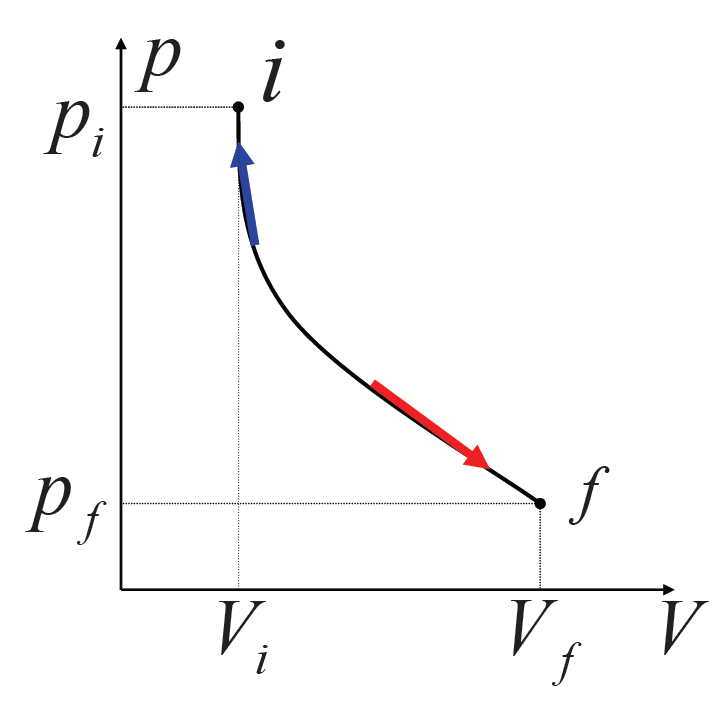
\includegraphics[width=0.35\textwidth]{reversible_process_pv.png}
\caption{可逆等温膨胀过程在 $p$-$V$ 图上的表示（需插入原PPT第15次课第3页图片）}
\label{fig:reversible_pv}
\end{figure}

\subsubsection*{不可逆过程举例}

\begin{itemize}
\item \textbf{有摩擦的准静态过程}；
\item \textbf{气体向真空的自由膨胀}：$i\to f$ 过程中 $\Delta U=0,\ W=0,\ Q=0$。尽管可以经一等温过程由 $f\to i$ 使系统复原，但此过程中 $W_{f\to i}>0,\ Q_{f\to i}<0$，外界未能复原；
\item \textbf{热传导过程}：高温 $\to$ 低温（自发）；低温 $\to$ 高温（需外力影响，如制冷机）；
\item \textbf{扩散过程}，及溶解、渗透等过程。
\end{itemize}

\textbf{核心判据}：\textbf{存在耗散、力学不平衡、热学不平衡、化学不平衡的过程都是不可逆过程}。

\begin{remark}
实际过程都是不可逆过程。可逆过程只是理想化的过程，或实际过程的近似。
\end{remark}

\begin{figure}[htbp]
\centering
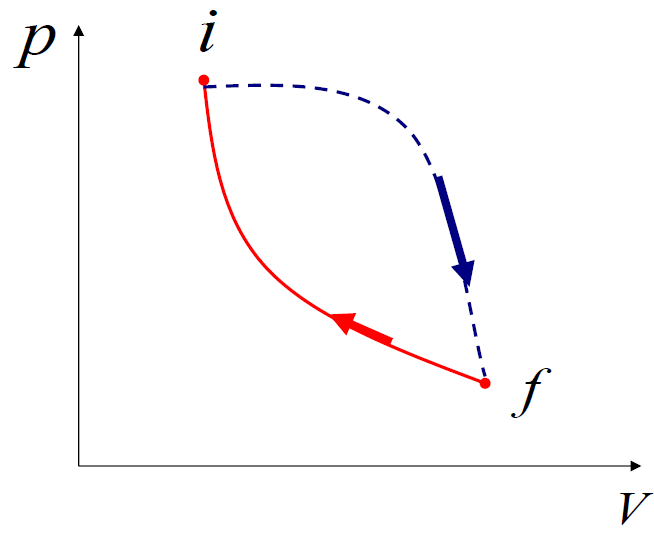
\includegraphics[width=0.35\textwidth]{irreversible_process_pv.png}
\caption{不可逆过程（如自由膨胀）在 $p$-$V$ 图上的表示（需插入原PPT第15次课第4页图片）}
\label{fig:irreversible_pv}
\end{figure}

% ----------------------------------------------
\subsection{热力学第二定律的两种语言表述}
% ----------------------------------------------

\subsubsection*{克劳修斯表述与开尔文表述}

热力学第二定律的两种经典语言表述如下：

\begin{itemize}
\item \textbf{克劳修斯表述}：不存在这样的过程，其唯一结果是将热量从低温物体传到高温物体。
\item \textbf{开尔文表述}：不存在这样的过程，其唯一结果是热量完全转化为功。
\end{itemize}

两种表述是等价的，它们分别从传热和做功两个角度揭示了热现象的不可逆性。

\subsubsection*{两种表述的等价性}

热力学第二定律的克劳修斯表述和开尔文表述\textbf{完全等价}。下面用反证法证明。

\textbf{证明}（克劳修斯表述 $\Rightarrow$ 开尔文表述）：

假设克劳修斯表述不成立，即存在某一过程 (a)，能使热量 $Q$ 从低温热源 $T_2$ 自动传到高温热源 $T_1$。将其与一卡诺热机 (b) 耦合：热机从 $T_1$ 吸热 $Q_1$，对外做功 $W'$，向 $T_2$ 放热 $Q$。则联合过程 (c) 的净效果为：从 $T_1$ 吸热 $Q_1-Q$，全部转化为功 $W'$，而未引起其他变化。这违背了开尔文表述。故克劳修斯表述若不对，则开尔文表述也不对。

\begin{figure}[htbp]
\centering
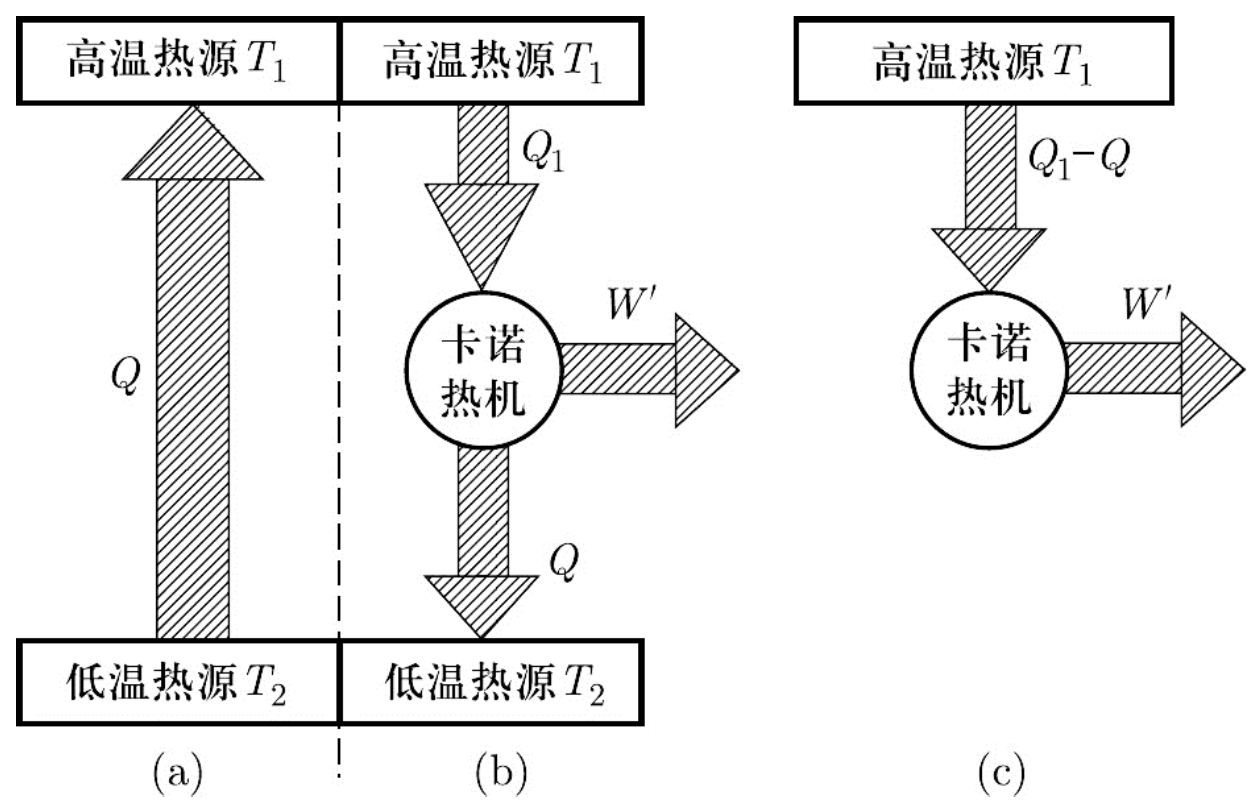
\includegraphics[width=0.6\textwidth]{equivalence_kelvin_clausius_1.png}
\caption{克劳修斯表述与开尔文表述等价性证明（一）（需插入原PPT第15次课第6页图片）}
\label{fig:equivalence1}
\end{figure}

\textbf{证明}（开尔文表述 $\Rightarrow$ 克劳修斯表述）：

同样用反证法。假设开尔文表述不成立，即存在某热机从高温热源 $T_1$ 吸热 $Q$，全部转化为功 $W'$。用此功驱动一制冷机，从低温热源 $T_2$ 吸热 $Q_2$，向 $T_1$ 放热 $Q_1$。则联合过程的净效果为：热量 $Q_1-Q=Q_2$ 从低温热源 $T_2$ 传到高温热源 $T_1$，而未引起其他变化。这违背了克劳修斯表述。

\begin{figure}[htbp]
\centering
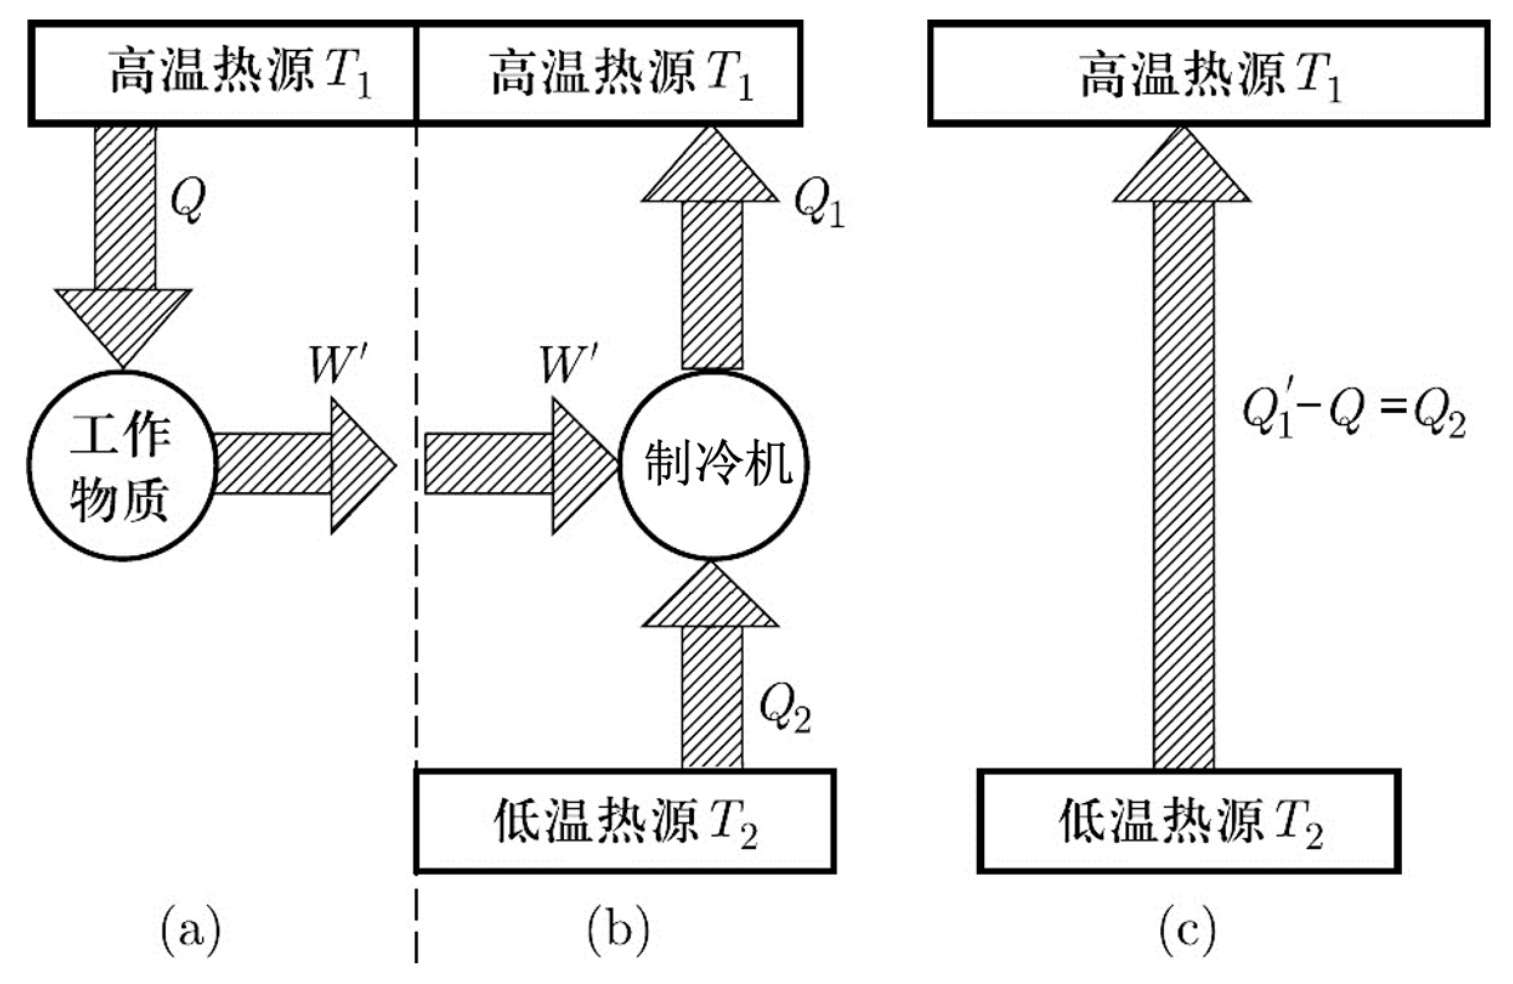
\includegraphics[width=0.6\textwidth]{equivalence_kelvin_clausius_2.png}
\caption{克劳修斯表述与开尔文表述等价性证明（二）（需插入原PPT第15次课第7页图片）}
\label{fig:equivalence2}
\end{figure}

\subsubsection*{热力学第二定律的实质}

对于自然现象的不可逆性，还可以有其他各种表述形式（如普朗克表述、奥斯特瓦尔德表述等）。

所有不可逆过程都是有联系的，从一种过程的不可逆性可以导出另一种过程的不可逆性，即它们是\textbf{等价的}。因此，这些表述都可以称为热力学第二定律。大家公认最早出现的克劳修斯表述和开尔文表述为热力学第二定律的传统的表述方式。

\textbf{热力学第二定律的实质}：\textbf{在一切与热相联系的自然现象中，它们自发实现的过程都是不可逆的}。

% ----------------------------------------------
\subsection{热力学第二定律的数学表述}
% ----------------------------------------------

\subsubsection*{卡诺定理}

卡诺定理是热力学第二定律的重要数学推论，包含两条核心结论：

\begin{enumerate}
\item 在相同的高温热源和相同的低温热源之间工作的一切\textbf{可逆热机}的效率都相等，与工作物质无关；
\item 在相同的高温热源和相同的低温热源之间工作的一切\textbf{不可逆热机}的效率 $\eta'$ 都小于可逆热机的效率 $\eta$。
\end{enumerate}

数学表达式为：
\begin{equation}
\boxed{\eta' = 1-\frac{Q_2'}{Q_1} < 1-\frac{T_2}{T_1} = \eta}
\end{equation}

\subsubsection*{卡诺定理的证明}

\textbf{（一）可逆热机效率相等}

设 A、B 都是可逆热机，一个循环中，它们从高温热源 $T_1$ 处吸热 $Q_{A1}$、$Q_{B1}$，对外作功 $W_A'$、$W_B'$，向低温热源 $T_2$ 放热 $Q_{A2}'$、$Q_{B2}'$。其效率分别为
\begin{equation}
\eta_A=\frac{W_A'}{Q_{A1}},\quad \eta_B=\frac{W_B'}{Q_{B1}}.
\end{equation}
设 $Q_{A1}=Q_{B1}$，由热力学第一定律
\begin{equation}
Q_{A1}=W_A'+Q_{A2}',\quad Q_{B1}=W_B'+Q_{B2}',
\end{equation}
可得
\begin{equation}
Q_{B2}'-Q_{A2}'=W_A'-W_B'.
\end{equation}

若假设 $\eta_A>\eta_B$，则 $W_A'>W_B'$，从而 $Q_{B2}'-Q_{A2}'>0$。考虑 ``A+B逆'' 组成的系统：$T_1$ 处净热量交换为零，系统从 $T_2$ 处吸收热量 $Q_{B2}'-Q_{A2}'$ 并全部转化为功，这违背了热力学第二定律的开尔文表述。故 $\eta_A>\eta_B$ 不成立。同理 $\eta_A<\eta_B$ 也不成立。因此
\begin{equation}
\eta_A=\eta_B.
\end{equation}

\begin{figure}[htbp]
\centering
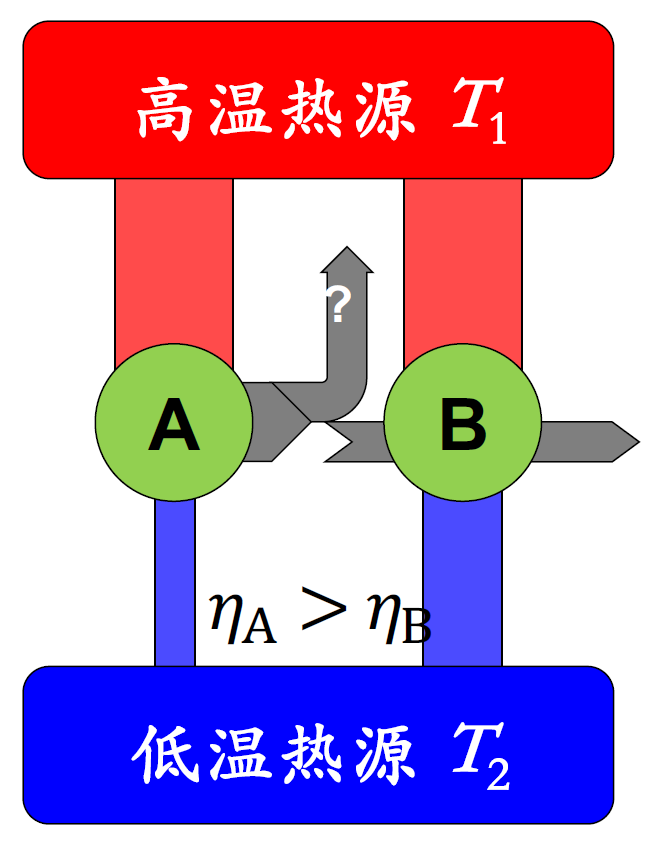
\includegraphics[width=0.35\textwidth]{carnot_theorem_proof_1.png}
\caption{卡诺定理证明（一）：两台可逆热机耦合（需插入原PPT第15次课第10页图片）}
\label{fig:carnot_proof1}
\end{figure}

\textbf{（二）不可逆热机效率小于可逆热机}

设 A 为不可逆热机，B 为可逆热机，且 $\eta_A>\eta_B$。若 $Q_{A1}=Q_{B1}$，同理可得
\begin{equation}
Q_{B2}'-Q_{A2}'=W_A'-W_B'>0.
\end{equation}
使 B 逆向运行（作为制冷机），则联合系统 A+B逆 将从低温热源 $T_2$ 吸热并全部转化为功，构成第二类永动机，违背热力学第二定律。故 $\eta_A>\eta_B$ 不成立，即
\begin{equation}
\eta_{\mathrm{IR}}\le\eta_{\mathrm{R}}.
\end{equation}

若 $\eta_A=\eta_B$，则 $Q_{B2}'-Q_{A2}'=0$，使 B 逆向运行后，系统 A+B逆 组成可逆机，这与 A 不可逆矛盾。因此
\begin{equation}
\eta_{\mathrm{IR}}\neq\eta_{\mathrm{R}}.
\end{equation}

综合得：
\begin{equation}
\boxed{\eta_{\mathrm{IR}} < \eta_{\mathrm{R}}}
\end{equation}

\begin{figure}[htbp]
\centering
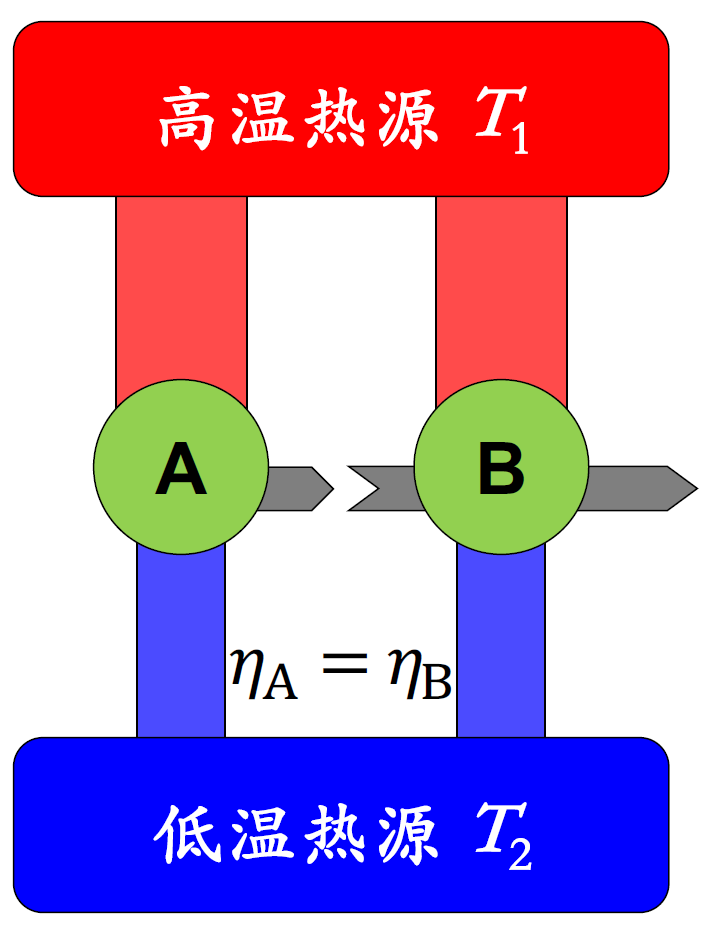
\includegraphics[width=0.35\textwidth]{carnot_theorem_proof_2.png}
\caption{卡诺定理证明（二）：不可逆热机与可逆热机比较（需插入原PPT第15次课第11页图片）}
\label{fig:carnot_proof2}
\end{figure}

\subsubsection*{克劳修斯不等式}

克劳修斯不等式是热力学第二定律的另一种数学表述。

（循环过程满足准静态假设，使得在不可逆过程中温度能够近似定义。）

\textbf{离散形式}：设一系统 $\Sigma$（任意工作物质）与 $n$ 个温度分别为 $T_1,T_2,\dots,T_n$ 的热源接触，经过一个循环，最后回到初始状态。在循环过程中各热源传递给系统的热量分别为 $Q_1,Q_2,\dots,Q_n$（系统对外界所作功记为 $W_\Sigma'$），则有
\begin{equation}
\boxed{\sum_{i=1}^{n}\frac{Q_i}{T_i}\le 0}
\end{equation}
等号适用于可逆循环。

\textbf{积分形式}：任意工作物质在一个循环过程中（可逆或不可逆），其热温比满足
\begin{equation}
\boxed{\oint\frac{\mathrm{d}Q}{T}\le 0}
\end{equation}
等号适用于可逆循环。

\subsubsection*{克劳修斯不等式的证明}

\textbf{1. 可逆卡诺循环}

对可逆卡诺循环，已知
\begin{equation}
\frac{Q_h}{Q_\ell}=\frac{T_h}{T_\ell}.
\end{equation}
定义在循环的每一个点进入系统的热量为 $\mathrm{d}Q_{\mathrm{rev}}$，则在一个循环中
\begin{equation}
\sum_{\mathrm{cycle}}\frac{\Delta Q_{\mathrm{rev}}}{T}=\frac{Q_h}{T_h}+\frac{(-Q_\ell)}{T_\ell}=0,
\end{equation}
即
\begin{equation}
\oint\frac{\mathrm{d}Q_{\mathrm{rev}}}{T}=0.
\end{equation}

\textbf{2. 推广到一般循环}

考虑运行在一系列热源之间的更一般循环，循环可以是可逆或不可逆的。在循环中的特定部分，系统和温度为 $T_i$ 的一个热源连接，热量 $\mathrm{d}Q_i$ 进入系统。整个循环对外做功
\begin{equation}
\Delta W=\sum_{\mathrm{cycle}}\mathrm{d}Q_i.
\end{equation}

\begin{figure}[htbp]
\centering
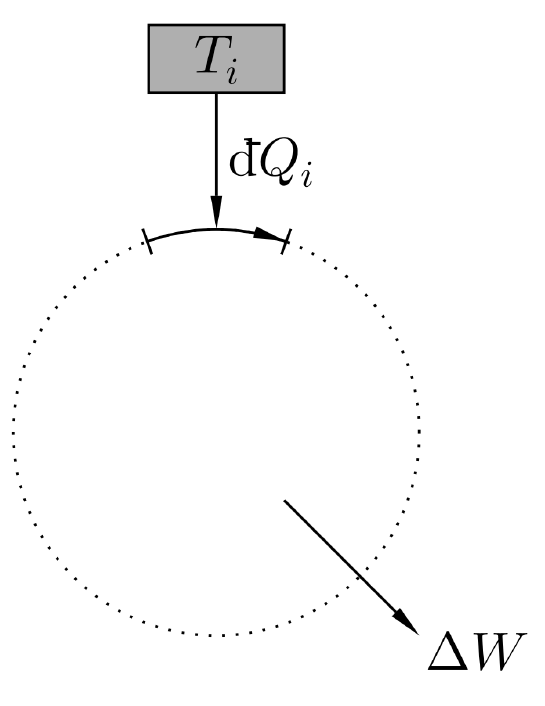
\includegraphics[width=0.35\textwidth]{general_cycle_diagram.png}
\caption{一般循环与多热源接触示意图（需插入原PPT第16次课第4页图片）}
\label{fig:general_cycle}
\end{figure}

设想在每个接触点，热量 $\mathrm{d}Q_i$ 由一个辅助卡诺热机提供。该卡诺热机工作于恒定高温热源 $T$ 与 $T_i$ 之间，满足
\begin{equation}
\frac{\mathrm{d}Q_i}{T_i}=\frac{\mathrm{d}Q_i+\mathrm{d}W_i}{T},
\quad\Rightarrow\quad
\mathrm{d}W_i=\mathrm{d}Q_i\left(\frac{T}{T_i}-1\right).
\end{equation}

所有辅助卡诺热机与原来循环联合工作的总效果，相当于一个从单一热源 $T$ 吸热并对外做功的循环。根据热力学第二定律，其总功不可能大于零：
\begin{equation}
\Delta W+\sum_{\mathrm{cycle}}\mathrm{d}W_i\le 0.
\end{equation}

将各关系代入整理，即得
\begin{equation}
\sum_{\mathrm{cycle}}\frac{\mathrm{d}Q_i}{T_i}\le 0
\quad\Rightarrow\quad
\oint\frac{\mathrm{d}Q}{T}\le 0.
\end{equation}

\begin{figure}[htbp]
\centering
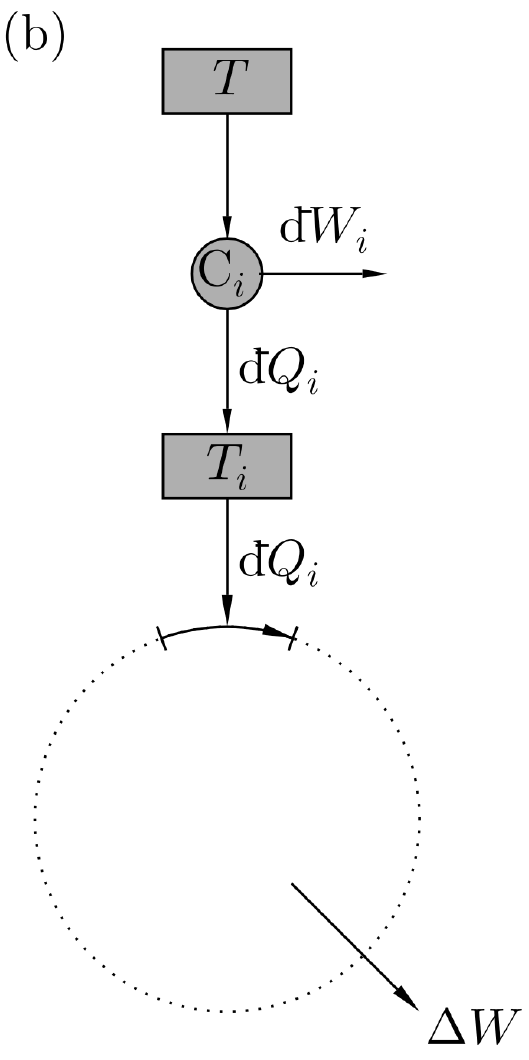
\includegraphics[width=0.25\textwidth]{carnot_heat_engine_aux.png}
\caption{克劳修斯不等式证明：辅助卡诺热机示意图（需插入原PPT第16次课第5页图片）}
\label{fig:carnot_aux}
\end{figure}

\subsubsection*{卡诺定理应用：非理想气体内能方程}

考虑一个\textbf{微小的卡诺正循环}：$AB$、$CD$ 为等温线；$BC$、$DA$ 为绝热线。循环足够小时，$ABCD$ 可近似看成平行四边形。

\begin{figure}[htbp]
\centering
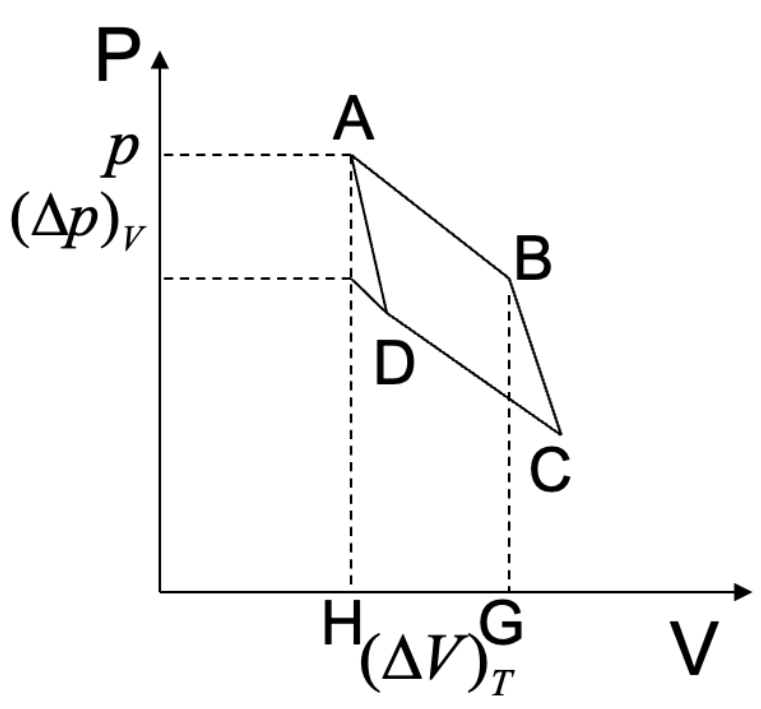
\includegraphics[width=0.35\textwidth]{infinitesimal_carnot_cycle.png}
\caption{微小卡诺循环在 $p$-$V$ 图上的表示（需插入原PPT第16次课第6页图片）}
\label{fig:infinitesimal_carnot}
\end{figure}

\textbf{对外做功}（循环曲线包围的面积）：
\begin{equation}
\Delta W_{\mathrm{total}}'=S_{ABCD}=(\Delta p)_V(\Delta V)_T.
\end{equation}

\textbf{从外吸热}（$AB$ 等温段）：
\begin{equation}
\Delta Q_{AB}=(\Delta U)_T+\Delta W_{AB}'=(\Delta U)_T+S_{ABGH}.
\end{equation}
其中
\begin{equation}
p_B=p-(\Delta p)_T,\quad
S_{ABGH}=\frac{1}{2}(\Delta V)_T(p+p_B)=(\Delta V)_T\left[p-\frac{1}{2}(\Delta p)_T\right].
\end{equation}
代入得
\begin{equation}
\Delta Q_{AB}=(\Delta V)_T\left[p-\frac{1}{2}(\Delta p)_T\right]+(\Delta U)_T.
\end{equation}

由卡诺定理，可逆循环效率
\begin{equation}
\eta=\frac{\Delta W'}{\Delta Q_{AB}}=\frac{\Delta T}{T}
\quad\Rightarrow\quad
\Delta W'=\frac{\Delta Q_{AB}\,\Delta T}{T}.
\end{equation}
将 $\Delta W'$ 与 $\Delta Q_{AB}$ 的表达式联立：
\begin{equation}
(\Delta p)_V(\Delta V)_T=\frac{\left\{(\Delta V)_T\left[p-\frac{1}{2}(\Delta p)_T\right]+(\Delta U)_T\right\}\Delta T}{T}.
\end{equation}

两边乘 $T$ 并除以 $(\Delta V)_T\Delta T$，令 $\Delta T\to 0$、$\Delta V\to 0$，取极限得
\begin{equation}
\boxed{\left(\frac{\partial U}{\partial V}\right)_T=T\left(\frac{\partial p}{\partial T}\right)_V-p}
\end{equation}
此即\textbf{内能方程}（又称能态方程），它将一般物质内能与物态方程联系起来。

\begin{remark}
对理想气体，$p=\dfrac{\nu RT}{V}$，代入得
\begin{equation}
\left(\frac{\partial U}{\partial V}\right)_T=T\frac{\nu R}{V}-p=0,
\end{equation}
说明理想气体内能只与温度有关，$U=U(T)$。
\end{remark}

% ----------------------------------------------
\subsection{熵与熵增加原理}
% ----------------------------------------------

\subsubsection*{熵的概念}

由克劳修斯不等式，对可逆循环有
\begin{equation}
\oint\frac{\mathrm{d}Q_{\mathrm{rev}}}{T}=0.
\end{equation}
这表明积分 $\displaystyle\int_A^B\frac{\mathrm{d}Q_{\mathrm{rev}}}{T}$ 与路径无关，因此 $\dfrac{\mathrm{d}Q_{\mathrm{rev}}}{T}$ 是一个\textbf{全微分}。

据此定义态函数\textbf{熵} $S$：
\begin{equation}
\boxed{\mathrm{d}S=\frac{\mathrm{d}Q_{\mathrm{rev}}}{T}}
\end{equation}
其积分形式为
\begin{equation}
S(B)-S(A)=\int_A^B\frac{\mathrm{d}Q_{\mathrm{rev}}}{T}.
\end{equation}

此即\textbf{克劳修斯熵}（宏观熵）。熵的数值可选取参考点（如标准状态）来确定。

\subsubsection*{热力学第二定律的另一种数学表述}

考虑一个不可逆过程，连接同样的初末态 $i$ 与 $f$。由于不可逆过程中 $\displaystyle\int\frac{\mathrm{d}Q}{T}$ 小于可逆过程的熵变，有
\begin{equation}
\int_{i\ \mathrm{IR}}^{f}\frac{\mathrm{d}Q}{T}<\int_{i\ \mathrm{R}}^{f}\frac{\mathrm{d}Q}{T}=S_f-S_i.
\end{equation}

\textbf{积分形式}：对任一过程，
\begin{equation}
\boxed{\int_i^f\frac{\mathrm{d}Q}{T}\le S_f-S_i}
\end{equation}

\textbf{微分形式}：对无穷小元过程，
\begin{equation}
\boxed{\mathrm{d}S\ge\frac{\mathrm{d}Q}{T}}
\end{equation}

等号仅适用于可逆过程。这就是热力学第二定律的数学表述，它表明：在不可逆过程中，系统的熵变大于热温比；在可逆过程中，熵变等于热温比。

\subsubsection*{热力学基本方程}

由热力学第一定律
\begin{equation}
\mathrm{d}Q=\mathrm{d}U-\mathrm{d}W.
\end{equation}
对于可逆过程：$\mathrm{d}Q=T\mathrm{d}S$，$\mathrm{d}W=-p\,\mathrm{d}V$。代入得
\begin{equation}
\mathrm{d}Q=\mathrm{d}U+p\,\mathrm{d}V=\mathrm{d}(U+pV)-V\,\mathrm{d}p=\mathrm{d}H-V\,\mathrm{d}p.
\end{equation}

两式联立，得到\textbf{热力学基本方程}（又称 $T\mathrm{d}S$ 方程）：
\begin{equation}
\boxed{T\mathrm{d}S=\mathrm{d}U+p\,\mathrm{d}V}
\qquad
\boxed{T\mathrm{d}S=\mathrm{d}H-V\,\mathrm{d}p}
\end{equation}

\begin{remark}
    热力学基本方程虽然由可逆过程导出，但由于式中各量均为态函数或其微分，故\textbf{对不可逆过程也成立}。
\end{remark}

\subsubsection*{熵变的计算}

\textbf{1. 以 $(T,V)$ 为自变量}

由 $T\mathrm{d}S=\mathrm{d}U+p\,\mathrm{d}V$，得
\begin{equation}
\mathrm{d}S=\frac{\mathrm{d}U}{T}+\frac{p}{T}\mathrm{d}V
=\frac{1}{T}\left[\left(\frac{\partial U}{\partial T}\right)_V\mathrm{d}T+\left(\frac{\partial U}{\partial V}\right)_T\mathrm{d}V\right]+\frac{p}{T}\mathrm{d}V.
\end{equation}
利用 $C_V=\left(\dfrac{\partial U}{\partial T}\right)_V$ 及内能方程，整理得
\begin{equation}
\mathrm{d}S=\frac{C_V}{T}\mathrm{d}T+\left(\frac{\partial p}{\partial T}\right)_V\mathrm{d}V.
\end{equation}
积分得
\begin{equation}
\Delta S=S_f-S_i=\int_i^f\frac{C_V}{T}\,\mathrm{d}T+\int_i^f\left(\frac{\partial p}{\partial T}\right)_V\mathrm{d}V.
\end{equation}

\textbf{2. 以 $(T,p)$ 为自变量}

由 $T\mathrm{d}S=\mathrm{d}H-V\,\mathrm{d}p$，类似可得
\begin{equation}
\mathrm{d}S=\frac{C_p}{T}\mathrm{d}T-\left(\frac{\partial V}{\partial T}\right)_p\mathrm{d}p,
\end{equation}
\begin{equation}
\Delta S=S_f-S_i=\int_i^f\frac{C_p}{T}\,\mathrm{d}T-\int_i^f\left(\frac{\partial V}{\partial T}\right)_p\mathrm{d}p.
\end{equation}

其中用到的辅助关系（可由麦克斯韦关系或直接用基本方程导出）：
\begin{equation}
\left(\frac{\partial H}{\partial p}\right)_T=-T\left(\frac{\partial V}{\partial T}\right)_p+V.
\end{equation}

\subsubsection*{理想气体熵变的计算}

对理想气体，$p=\dfrac{\nu RT}{V}$，$V=\dfrac{\nu RT}{p}$，代入上述一般公式。

\textbf{以 $(T,V)$ 为自变量}：
\begin{equation}
\left(\frac{\partial p}{\partial T}\right)_V=\frac{\nu R}{V},
\end{equation}
\begin{equation}
S(T,V)=\int_{T_0}^{T}\frac{C_V}{T}\,\mathrm{d}T+\int_{V_0}^{V}\frac{\nu R}{V}\,\mathrm{d}V+S_0
=C_V\ln\frac{T}{T_0}+\nu R\ln\frac{V}{V_0}+S_0.
\end{equation}

\textbf{以 $(T,p)$ 为自变量}：
\begin{equation}
\left(\frac{\partial V}{\partial T}\right)_p=\frac{\nu R}{p},
\end{equation}
\begin{equation}
S(T,p)=\int_{T_0}^{T}\frac{C_p}{T}\,\mathrm{d}T-\int_{p_0}^{p}\frac{\nu R}{p}\,\mathrm{d}p+S_0
=C_p\ln\frac{T}{T_0}-\nu R\ln\frac{p}{p_0}+S_0.
\end{equation}

\textbf{几种典型可逆过程的熵变}：

\begin{itemize}
\item \textbf{可逆等温过程}（$T=\text{常量}$）：
\begin{equation}
\Delta S=\nu R\ln\frac{V_f}{V_i}=-\nu R\ln\frac{p_f}{p_i}.
\end{equation}

\item \textbf{可逆绝热过程}（$\mathrm{d}Q=0$）：
\begin{equation}
\mathrm{d}S=\frac{\mathrm{d}Q}{T}=0,\quad\Rightarrow\quad\Delta S=0.
\end{equation}

\item \textbf{可逆等压过程}（$p=\text{常量}$）：
\begin{equation}
\Delta S=C_p\ln\frac{T_f}{T_i}.
\end{equation}

\item \textbf{可逆等体过程}（$V=\text{常量}$）：
\begin{equation}
\Delta S=C_V\ln\frac{T_f}{T_i}.
\end{equation}
\end{itemize}

\subsubsection*{可逆多方过程的熵变}

对可逆多方过程，$pV^n=\text{const}$，结合理想气体状态方程 $pV=\nu RT$，可得
\begin{equation}
V=\text{const}\cdot(\nu RT)^{\frac{1}{1-n}}.
\end{equation}

将其代入以 $(T,V)$ 为自变量的熵变公式：
\begin{equation}
\Delta S=C_V\ln\frac{T_f}{T_i}+\nu R\ln\frac{V_f}{V_i}
=C_V\ln\frac{T_f}{T_i}+\nu R\ln\left(\frac{T_f}{T_i}\right)^{\frac{1}{1-n}}
=\left[C_V+\frac{\nu R}{1-n}\right]\ln\frac{T_f}{T_i}.
\end{equation}

利用 $\nu R=C_p-C_V$ 及 $\gamma=C_p/C_V$，上式可进一步化为
\begin{equation}
\Delta S=\frac{C_p-nC_V}{1-n}\ln\frac{T_f}{T_i}
=\frac{\gamma-n}{1-n}C_V\ln\frac{T_f}{T_i}
=C_n\ln\frac{T_f}{T_i},
\end{equation}
其中 $C_n=\dfrac{\gamma-n}{1-n}C_V$ 为多方热容（参见第四章PPT）。

\begin{remark}
不同过程的熵计算公式不同并不表示熵是过程量，而是因为过程的终态不一样。
\end{remark}

\subsubsection*{不可逆过程中熵变的计算}

不可逆过程的熵变不能直接沿不可逆路径积分求得，而应采用间接途径：

\begin{enumerate}
\item 设计一个连接相同的初态和相同的末态的\textbf{可逆路径}，根据态函数的性质，通过计算该可逆过程的熵变求得不可逆过程的熵变；
\item 设熵函数的参考点 $S_0(T_0,V_0)$ 或 $S_0(T_0,p_0)$，计算熵作为\textbf{态函数}的形式 $S(T,V)$ 或 $S(T,p)$，再把初末态状态参量代入计算熵变。
\end{enumerate}

例如，对理想气体：
\begin{equation}
S(T,V)=C_V\ln\frac{T}{T_0}+\nu R\ln\frac{V}{V_0}+S_0,\qquad
S(T,p)=C_p\ln\frac{T}{T_0}-\nu R\ln\frac{p}{p_0}+S_0.
\end{equation}

\subsubsection*{自由膨胀过程的熵变}

理想气体由初态 $i$ 自由膨胀到末态 $f$：$Q=0,\ W=0$，且因理想气体内能只与温度有关，故 $T_f=T_i$。此过程\textbf{不可逆}。

\textbf{计算途径（1）：设计可逆等温过程}

在 $p$-$V$ 图上连接初末态作可逆等温线，则
\begin{equation}
\Delta S=\nu R\ln\frac{V_f}{V_i}=-\nu R\ln\frac{p_f}{p_i}>0.
\end{equation}

\textbf{计算途径（2）：可逆绝热过程 + 可逆等体过程}

先经可逆绝热过程由 $i\to m$，再经可逆等体过程由 $m\to f$：
\begin{itemize}
\item 可逆绝热过程：$\Delta S|_{ad}=0$；
\item 可逆等体过程：$\displaystyle\Delta S=\Delta S|_V=C_V\ln\frac{T_f}{T_m}$。
\end{itemize}

由状态方程 $T_f=\dfrac{p_fV_f}{\nu R},\ T_m=\dfrac{p_mV_f}{\nu R}$，得
\begin{equation}
\frac{T_f}{T_m}=\frac{p_f}{p_m}=\frac{p_f}{p_i}\left(\frac{V_f}{V_i}\right)^{\gamma},
\end{equation}
其中利用了绝热过程关系 $p_mV_f^{\gamma}=p_iV_i^{\gamma}$（即 $V_m=V_f$）以及自由膨胀中 $p_iV_i=p_fV_f$（$T_f=T_i$）。

于是
\begin{align}
\Delta S&=C_V\ln\frac{T_f}{T_m}
=C_V\ln\frac{p_f}{p_i}+\gamma C_V\ln\frac{V_f}{V_i} \notag\\
&=(\gamma-1)C_V\ln\frac{V_f}{V_i}
=\nu R\ln\frac{V_f}{V_i}.
\end{align}

引入膨胀比 $n=\dfrac{V_f}{V_i}>1$，则不论以什么状态参量表示熵，自由膨胀过程中理想气体的熵变均为
\begin{equation}
\boxed{\Delta S_{FE}=\nu R\ln n>0.}
\end{equation}

\subsubsection*{气体混合过程的熵变}

设混合气体为理想气体，$c_j=\nu_j/\nu$ 是第 $j$ 种组分的摩尔百分比，温度为 $T$，体积为 $V$，总压强 $p=\sum_j p_j$，其中第 $j$ 种组分的分压强为 $p_j=c_j p$。未混合时，各组分的温度均为 $T$，压强均为 $p$，各自占有体积 $V_j=c_j V$，然后在总体积、总压强和温度均不变的情况下混合。

\textbf{计算途径（1）：等温膨胀过程}

每个组分从 $V_j=c_j V$ 等温膨胀到总体积 $V$：
\begin{equation}
\Delta S_j=c_j\nu R\ln\frac{V}{V_j},\qquad
\Delta S=\sum_j\Delta S_j=-\nu R\sum_j c_j\ln\frac{V_j}{V}
=-\nu R\sum_j c_j\ln c_j>0.
\end{equation}

\textbf{计算途径（2）：等温变压过程}

每个组分从压强 $p$ 等温变化到分压 $p_j=c_j p$：
\begin{equation}
\Delta S_j=-c_j\nu R\ln\frac{p_j}{p},\qquad
\Delta S=\sum_j\Delta S_j=-\nu R\sum_j c_j\ln\frac{p_j}{p}
=-\nu R\sum_j c_j\ln c_j>0.
\end{equation}

% --------------------------------------------
\subsection{热传递过程中熵变}
% --------------------------------------------

\subsubsection*{等压传热熵变计算}

如图，物体（$T_A$）与热库（$T_B$）接触，等压条件下吸收热量$Q=C_p(T_B-T_A)$，达到温度$T_B$，物体与热库组成的系统是孤立的，过程为绝热过程。

\begin{figure}[htbp]
\centering
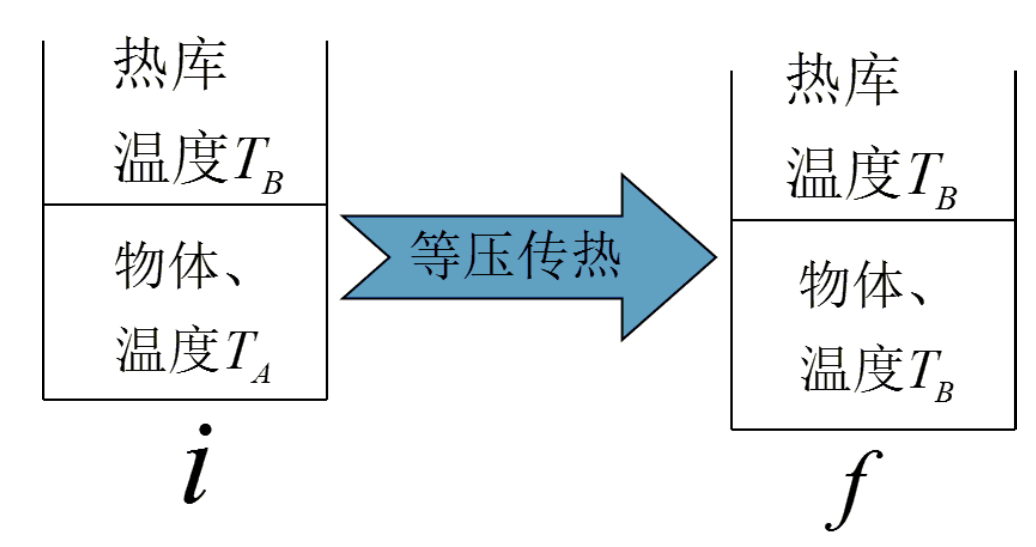
\includegraphics[width=0.4\textwidth]{heat_transfer_entropy.png}
\caption{物体与热库等压传热过程示意图（需插入原PPT第17次课第2页图片）}
\label{fig:heattransfer}
\end{figure}

\begin{align}
\Delta S_{\text{物体}} &= C_p\ln\frac{T_f}{T_i} - \nu R\ln\frac{p_f}{p_i} = C_p\ln\frac{T_B}{T_A} \\
\Delta S_{\text{热库}} &= \int_i^f \frac{\mathrm{d}Q}{T} = \frac{1}{T_B}\int_i^f -C_p\,\mathrm{d}T = \frac{1}{T_B}\bigl[-C_p(T_B-T_A)\bigr] = -C_p\frac{T_B-T_A}{T_B} \\
\Delta S_{\text{系统}} &= \Delta S_{\text{物体}} + \Delta S_{\text{热库}} = C_p\Bigl[\ln\frac{T_B}{T_A} - \frac{T_B-T_A}{T_B}\Bigr]
\end{align}

当$T_B>T_A$时，
\begin{equation}
\ln\frac{T_B}{T_A} = \int_{T_A}^{T_B}\frac{\mathrm{d}T}{T} > \int_{T_A}^{T_B}\frac{\mathrm{d}T}{T_B} = \frac{T_B-T_A}{T_B}
\end{equation}

当$T_B<T_A$时，
\begin{equation}
\ln\frac{T_A}{T_B} = \int_{T_B}^{T_A}\frac{\mathrm{d}T}{T} < \int_{T_B}^{T_A}\frac{\mathrm{d}T}{T_B} = \frac{T_A-T_B}{T_B}
\quad\Rightarrow\quad
\ln\frac{T_B}{T_A} > \frac{T_B-T_A}{T_B}
\end{equation}

无论$T_B>T_A$或$T_A>T_B$，都有$\displaystyle\ln\frac{T_B}{T_A} > \frac{T_B-T_A}{T_B}$，故
\begin{equation}
\boxed{\Delta S_{\text{系统}} = C_p\Bigl[\ln\frac{T_B}{T_A} - \frac{T_B-T_A}{T_B}\Bigr] > 0}
\end{equation}

% --------------------------------------------
\subsection{熵增加原理}
% --------------------------------------------

\subsubsection*{一般推导}

初态$i$到末态$f$有各种路径，设$p$-$V$图上$L$是讨论的过程（可逆或不可逆），选另一连接$i$和$f$的\textbf{可逆路径}$L_0$，则$(L+\text{逆}L_0)$构成一个循环，由\textbf{克劳修斯不等式}
\begin{equation}
\oint\frac{\mathrm{d}Q}{T} = \int_L\frac{\mathrm{d}Q}{T} + \int_{-L_0}\frac{\mathrm{d}Q}{T} \le 0
\quad\text{即}\quad
\int_L\frac{\mathrm{d}Q}{T} \le \int_{L_0}\frac{\mathrm{d}Q}{T}
\end{equation}

$i$到$f$的过程中熵变为
\begin{equation}
\Delta S_L = \int_{L_0}\frac{\mathrm{d}Q}{T} \ge \int_L\frac{\mathrm{d}Q}{T}
\end{equation}
路径$L$任意，$\mathrm{d}Q$可正可负，所以$\displaystyle\Delta S_L \ge \int_L\frac{\mathrm{d}Q}{T}$可正可负。

对绝热过程$L$则有
\begin{equation}
\Delta S_{ad} \ge \int_{ad}\frac{\mathrm{d}Q}{T} = 0
\quad\Rightarrow\quad
\boxed{\Delta S_{ad} \ge 0}
\end{equation}

\begin{figure}[htbp]
\centering
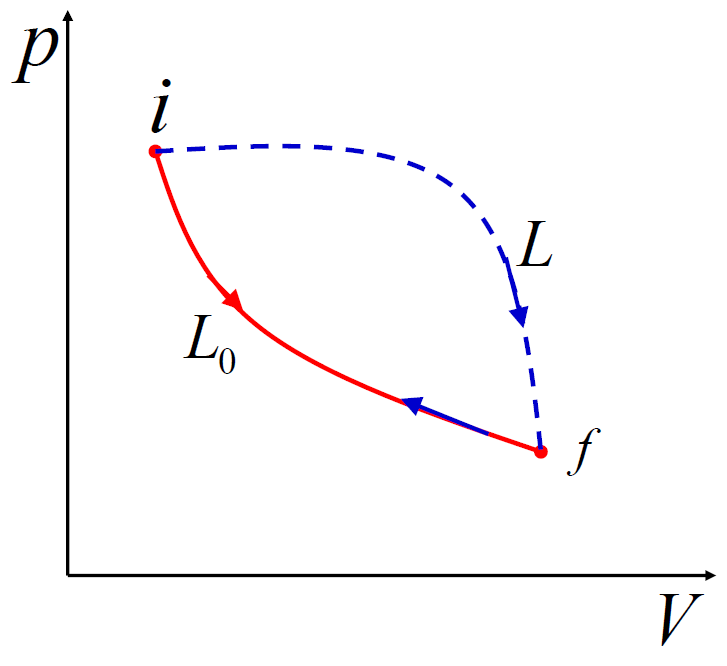
\includegraphics[width=0.35\textwidth]{entropy_increase_pv.png}
\caption{熵增加原理：不可逆路径$L$与可逆路径$L_0$构成的循环（需插入原PPT第17次课第4页图片）}
\label{fig:entropypv}
\end{figure}

\subsubsection*{熵增加原理的表述与讨论}

实例计算和一般计算都表明，在\textbf{绝热过程中}
\begin{equation}
\boxed{\Delta S \ge 0}
\end{equation}

\begin{remark}
热力学系统从一个平衡态经\textbf{绝热过程}到达另一个平衡态，它的熵永不减少。若过程可逆，则其熵不变；若过程不可逆，则其熵增加。
\end{remark}

判断绝热过程是否可逆，实际计算熵变：
\begin{itemize}
\item 若$\Delta S > 0$则该绝热过程\textbf{不可逆}；
\item 若$\Delta S = 0$则该绝热过程\textbf{可逆}。
\end{itemize}

克劳修斯不等式的另一种表述：
\begin{equation}
T\,\mathrm{d}S \ge \mathrm{d}Q \quad (\text{可逆取等号})
\end{equation}

\begin{itemize}
\item \textbf{熵增加原理}是孤立系统绝热过程进行方向的判据（时间箭头）：$\Delta S \ge 0$；
\item 孤立系统热平衡的判据：熵取得极大值，即$\mathrm{d}S = 0$；
\item 严格地，在内能和体积不变的条件下，对于一切可能的变动来说，平衡态的熵最大，此时$\mathrm{d}S = 0$。
\end{itemize}

\subsubsection*{例题：三物体热机问题}

\textbf{题目}：三个热容都为$C$（可近似为常量）的相同物体，其温度分别为$T_A=T_B=300\,\mathrm{K}$，$T_C=100\,\mathrm{K}$。若外界不作功，也不传热，利用热机将三个物体作为热源，使其中的某一个温度升高，试问它所能达到的最高温度为多少？此时其它两物体温度各为多少？

\textbf{解}：设温度改变后，三物体的温度分别为$T_A'$、$T_B'$、$T_C'$。因为对三物体既不作功、也不传热，则对三物体组成的系统，必有
\begin{equation}
\Delta U = C\Delta T_A + C\Delta T_B + C\Delta T_C = 0
\quad\text{即}\quad
T_A'+T_B'+T_C' = T_A+T_B+T_C = 700\,\mathrm{K}
\end{equation}

对三物体组成的孤立系统，该过程\textbf{可逆}，则根据熵增加原理：
\begin{equation}
\Delta S = \int_{T_A}^{T_A'}\frac{C\,\mathrm{d}T}{T} + \int_{T_B}^{T_B'}\frac{C\,\mathrm{d}T}{T} + \int_{T_C}^{T_C'}\frac{C\,\mathrm{d}T}{T} = 0
\end{equation}
即
\begin{equation}
\ln\frac{T_A'}{T_A} + \ln\frac{T_B'}{T_B} + \ln\frac{T_C'}{T_C} = 0
\quad\Rightarrow\quad
T_A'\cdot T_B'\cdot T_C' = T_A\cdot T_B\cdot T_C = 9\times10^6\,\mathrm{K}^3
\end{equation}

依题意，工作方式可能是$B$与$C$之间有一热机，其输出功$W$驱动$B$与$A$之间的制冷机将热量再从$B$传输到$A$。$A$物体最后达到的温度最高，有：$T_B' = T_C' < T_A'$。

\begin{figure}[htbp]
\centering
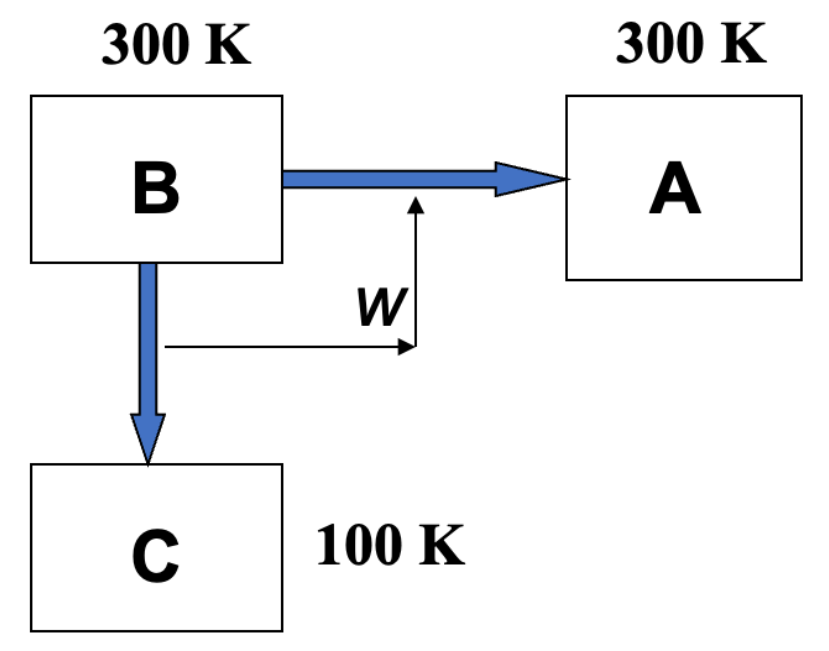
\includegraphics[width=0.4\textwidth]{three_body_heat_engine.png}
\caption{三物体热机与制冷机工作方式示意图（需插入原PPT第17次课第8页图片）}
\label{fig:threebody}
\end{figure}

代入前两式：
\begin{align}
T_A' + 2T_B' &= 700 \\
T_A'\cdot T_B'^2 &= 9\times10^6
\end{align}
从两式可得：$2T_B'^3 - 700T_B'^2 + 9\times10^6 = 0$。

解得三组解：
\begin{equation*}
\begin{cases}
T_A' = 400\,\mathrm{K},\quad T_B'=T_C'=150\,\mathrm{K} \\[4pt]
T_A' = 100\,\mathrm{K},\quad T_B'=T_C'=300\,\mathrm{K} \\[4pt]
T_A' = 900\,\mathrm{K},\quad T_B'=T_C'=-100\,\mathrm{K}
\end{cases}
\end{equation*}
显然，只有第一组解合理。

% --------------------------------------------
\subsection{熵及热力学第二定律的统计意义}
% --------------------------------------------

\subsubsection*{玻尔兹曼熵}

\textbf{玻尔兹曼熵}：
\begin{equation}
\boxed{S_B = k_B\ln\Omega}
\end{equation}
其中$k_B$为玻尔兹曼常数，$\Omega$为系统的微观态数目。

热物理量可分为\textbf{强度量}和\textbf{广延量}两类，但$\Omega$不能归入上述两类。然而，
\begin{equation}
\ln\Omega_{A+B} = \ln(\Omega_A\cdot\Omega_B) = \ln\Omega_A + \ln\Omega_B
\end{equation}
即$\ln\Omega$是\textbf{广延量}，且与$\Omega$有相同的单调性质。所以，可用上定义描述热力学系统的微观态及其性质。这样定义的$S$即称为微观熵，或玻尔兹曼熵，记为$S_B$。

\textbf{宏观熵与微观熵的关系}为
\begin{equation}
\boxed{\Delta S_C = \Delta S_B}
\end{equation}

\subsubsection*{微观熵与宏观熵的关系}

玻尔兹曼系统的微观态数目
\begin{equation}
\Omega = \frac{N!}{\prod_i N_i!}\prod_i g_i^{N_i}
\end{equation}
对简单情况，$g_i=1$，则$\displaystyle\Omega = \frac{N!}{\prod_i N_i!}$。

\begin{equation}
\ln\Omega = \ln N! - \ln\prod_i N_i! = \ln N! - \sum_i\ln N_i!
\end{equation}

粒子数守恒，
\begin{equation}
\mathrm{d}\ln\Omega = -\sum_i\mathrm{d}\ln N_i! = -\sum_i\mathrm{d}[N_i\ln N_i - N_i] = -\sum_i\ln N_i\,\mathrm{d}N_i
\end{equation}

最可几分布为\textbf{玻尔兹曼分布}：$N_i = e^{-\alpha-\beta\varepsilon_i}$，故$\ln N_i = -\alpha-\beta\varepsilon_i = \ln N_0 - \beta\varepsilon_i$。

\begin{equation}
\mathrm{d}\ln\Omega = -\sum_i(\ln N_0 - \beta\varepsilon_i)\,\mathrm{d}N_i = -\ln N_0\sum_i\mathrm{d}N_i + \beta\sum_i\varepsilon_i\,\mathrm{d}N_i = \beta\sum_i\varepsilon_i\,\mathrm{d}N_i
\end{equation}

由热力学第一定律知
\begin{equation}
\mathrm{d}E = \mathrm{d}\sum_i N_i\varepsilon_i = \sum_i\varepsilon_i\,\mathrm{d}N_i + \sum_i N_i\,\mathrm{d}\varepsilon_i = \mathrm{d}Q + \mathrm{d}W
\end{equation}

\begin{equation}
\mathrm{d}\ln\Omega = \beta\sum_i\varepsilon_i\,\mathrm{d}N_i = \beta\,\mathrm{d}Q,\qquad
\mathrm{d}S_B = k_B\,\mathrm{d}(\ln\Omega) = \frac{\mathrm{d}Q}{T}
\end{equation}

\begin{equation}
\mathrm{d}S_C = \frac{\mathrm{d}Q}{T} = \mathrm{d}S_B
\quad\Rightarrow\quad
\boxed{\Delta S_C = \Delta S_B}
\end{equation}

\subsubsection*{实例检验}

\textbf{自由膨胀}

系统初态$i$和末态$f$的微观态数分别为$\Omega_i$、$\Omega_f$，在$i\to f$过程中
\begin{equation}
\Delta S_B = S_{B,f} - S_{B,i} = k_B\ln(\Omega_f/\Omega_i)
\end{equation}

膨胀前微观态数$\Omega_i=1$；膨胀后，系统中有$N=\nu N_A$个粒子，每个粒子处于左右两边概率都是$1/2$，总微观态数$\Omega_f = 2^N$。

\begin{figure}[htbp]
\centering
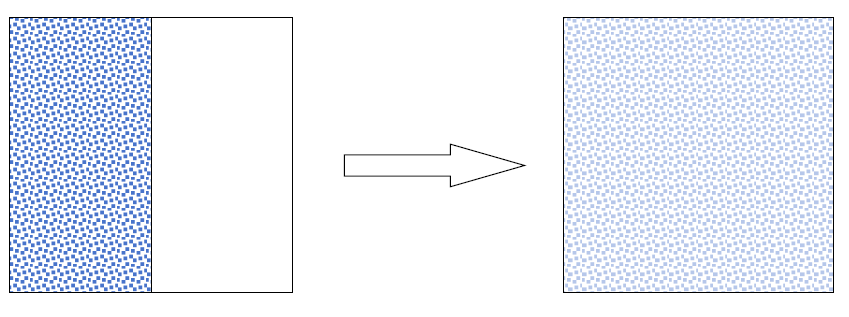
\includegraphics[width=0.55\textwidth]{free_expansion_microstates.png}
\caption{自由膨胀过程微观态示意图（需插入原PPT第17次课第12页图片）}
\label{fig:freemicro}
\end{figure}

\begin{equation}
\Delta S_B = k_B\ln\frac{\Omega_f}{\Omega_i} = k_B\ln 2^N = k_B N\ln 2 = \nu R\ln 2 = \nu R\ln\left(\frac{V_f}{V_i}\right) = \Delta S_C
\end{equation}

\textbf{混合过程}

混合系统中$X$、$Y$组分的摩尔浓度为$C_X$、$C_Y$，粒子数为$N_X$、$N_Y$，总的微观态数目为$\Omega_t$，总的物质的量为$\nu$。

\begin{figure}[htbp]
\centering
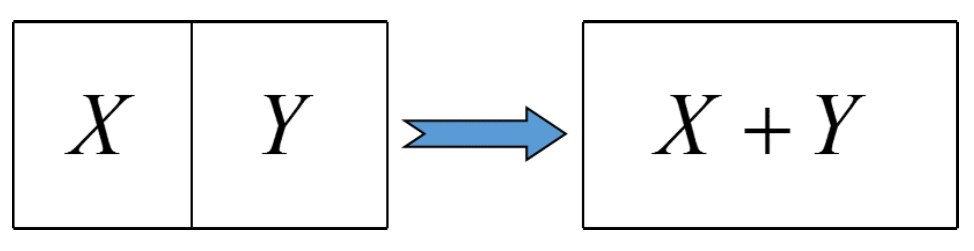
\includegraphics[width=0.55\textwidth]{mixing_process.png}
\caption{混合过程示意图（需插入原PPT第17次课第13页图片）}
\label{fig:mixing}
\end{figure}

扩散前微观态数目：$\Omega_i = [C_X^{N_X}C_Y^{N_Y}]\Omega_t$

扩散后微观态数目：$\Omega_f = \Omega_t$

\begin{align}
\Delta S_B &= k_B\ln\frac{\Omega_f}{\Omega_i} = k_B\ln\frac{1}{C_X^{N_X}C_Y^{N_Y}} = -k_B\ln\!\left(C_X^{N_X}C_Y^{N_Y}\right) = -k_B\bigl(N_X\ln C_X + N_Y\ln C_Y\bigr) \\
&= -k_B N_A(\nu_X\ln C_X + \nu_Y\ln C_Y) = -\nu R\bigl(C_X\ln C_X + C_Y\ln C_Y\bigr) = \Delta S_C
\end{align}

\subsubsection*{统计意义的总结}

$\Omega$是系统的微观状态数，是系统内部无序程度的度量。所以，\textbf{熵是系统宏观状态对应的微观状态的多少（即无序程度）的度量}。

\textbf{熵高}意味着对应的\textbf{微观状态数目多}，即混乱、分散、无序程度高。

根据\textbf{微观状态等几率基本假设}，微观状态数最多的宏观状态出现的概率最大；

\textbf{熵低}意味着对应的\textbf{微观状态数目少}，即整齐、集中、无序程度低。根据微观状态等几率基本假设，微观状态数较少的宏观状态出现的概率较小；

\textbf{熵增加}是系统从\textbf{有序到无序}的过程；其伴随的能量传递过程对应为\textbf{有用}（有序）能量减少，\textbf{无用}（无序）能量增多。

如：自由膨胀；扩散；固液、固气、液气相变；向米里掺沙子；功转变为热……

% --------------------------------------------
\subsection{热力学第二定律的应用：热力学温标的建立}
% --------------------------------------------

\subsubsection*{卡诺定理与普适函数}

\textbf{卡诺定理}：工作于两温度恒定的热源之间的一切可逆卡诺热机的效率与工作物质无关，只是温度的函数。此函数一定是普适的，其形式的选取决定温标的制定，可以建立与测温物质无关的热力学温标。

设两热源温度分别为$\Theta_1$、$\Theta_2$，卡诺热机分别在其处吸放热$Q_1$、$Q_2'$，则由$\eta = 1 - Q_2'/Q_1$与工作物质无关知
\begin{equation}
\frac{Q_2'}{Q_1} = 1-\eta = f(\Theta_1,\Theta_2)
\end{equation}
其中$f(\Theta_1,\Theta_2)$是两温度$\Theta_1$、$\Theta_2$的普适函数。

以下证明此普适函数满足：
\begin{equation}
f(\Theta_3,\Theta_1)f(\Theta_1,\Theta_2) = f(\Theta_3,\Theta_2)
\end{equation}

设在温度分别为$\Theta_1$、$\Theta_2$的两热源外有另一温度为$\Theta_3$热源，$\Theta_3$和$\Theta_2$之间置一可逆卡诺热机，在一个循环中，从$\Theta_3$处吸热$Q_3$，在$\Theta_2$处放热$Q_2'$，则
\begin{equation}
\frac{Q_2'}{Q_3} = f(\Theta_3,\Theta_2)
\end{equation}

置一可逆卡诺热机工作于$\Theta_3$和$\Theta_1$间，在一个循环中，它从$\Theta_3$处吸热$Q_3$，在$\Theta_1$处放热$Q_1'$，则
\begin{equation}
\frac{Q_1'}{Q_3} = f(\Theta_3,\Theta_1)
\end{equation}

第三个热机在$\Theta_1$处吸热$Q_1$，在$\Theta_2$处放热$Q_2'$，因为卡诺热机效率相等，适当调节此热机可得
\begin{equation}
\frac{Q_2'}{Q_1}\cdot\frac{Q_1'}{Q_3} = \frac{Q_2'}{Q_3}
\quad\Rightarrow\quad
f(\Theta_1,\Theta_2) = \frac{f(\Theta_3,\Theta_2)}{f(\Theta_3,\Theta_1)}
\end{equation}

\begin{figure}[htbp]
\centering
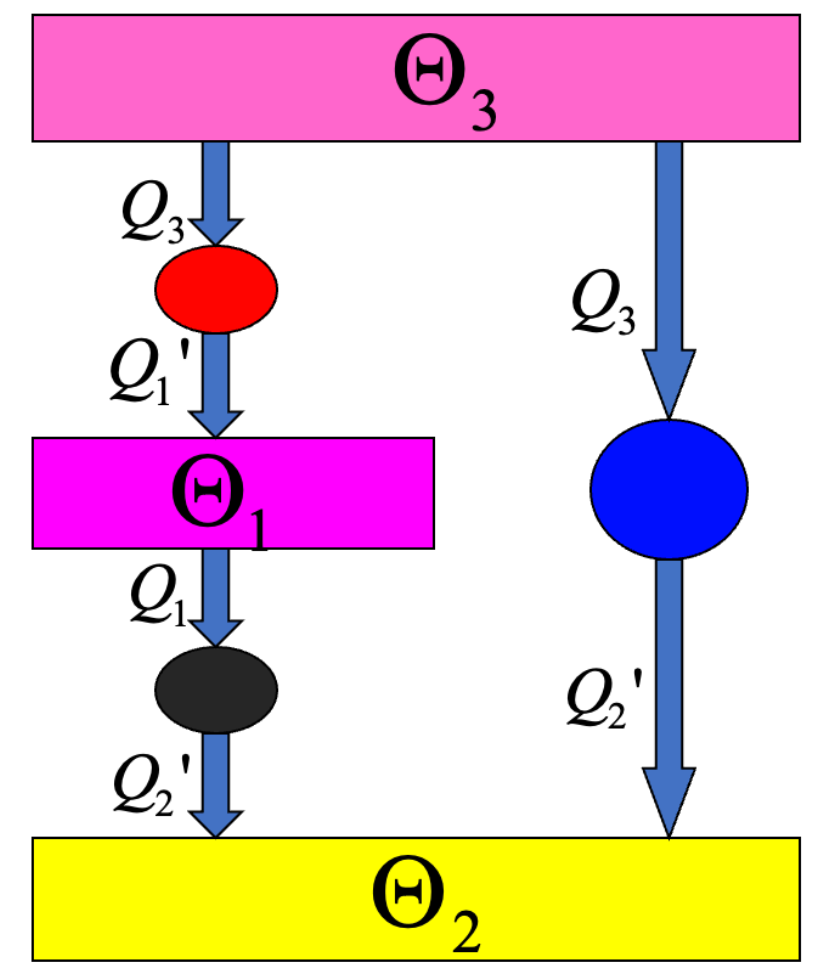
\includegraphics[width=0.35\textwidth]{thermodynamic_temperature_carnot.png}
\caption{三热源可逆卡诺热机建立热力学温标示意图（需插入原PPT第18次课第3页图片）}
\label{fig:carnot3}
\end{figure}

\subsubsection*{热力学温标的建立}

\begin{itemize}
\item $f(\Theta_1,\Theta_2)$与$\Theta_3$无关，$\displaystyle\frac{f(\Theta_3,\Theta_2)}{f(\Theta_3,\Theta_1)} = f(\Theta_1,\Theta_2)$也与$\Theta_3$无关。
\item $f$必可\textbf{因子化}：$\displaystyle f(\Theta_1,\Theta_2) = \frac{\Psi(\Theta_2)}{\Psi(\Theta_1)}$，$\Psi$为另一普适函数。
\item 选不同形式的$\Psi(\Theta)$即可定义不同的温标，如$\Psi(\Theta)=\Theta$，则有$\displaystyle\frac{Q_2'}{Q_1} = f(\Theta_1,\Theta_2) = \frac{\Theta_2}{\Theta_1} = \frac{T_2}{T_1}$。
\end{itemize}

这样定义的温标与测温物质无关，是普适的。所以称为\textbf{热力学温标}或\textbf{绝对温标}。它仅定义了两温度的比值，需要再规定固定标准点。

\textbf{固定点}：1954年国际计量大会：水三相点为$273.16\,\mathrm{K}$。

热力学温度单位：开尔文($\mathrm{K}$)，$\displaystyle 1\,\mathrm{K} = \frac{1}{273.16}\times$水三相点热力学温度。

\subsubsection*{热力学温标与实际温标的关系}

只要知道用实际温标表示的测温物质状态方程$p(\theta,V)$与内能方程$U(\theta,V)$，就可以确定此温标与热力学温标的关系。

内能方程
\begin{equation}
\left(\frac{\partial U}{\partial V}\right)_T = T\left(\frac{\partial p}{\partial T}\right)_V - p
\end{equation}
$\theta$是$T$的单调函数。

\begin{equation}
T\left(\frac{\partial p}{\partial T}\right)_V = T\left(\frac{\partial p}{\partial\theta}\right)_V\left(\frac{\mathrm{d}\theta}{\mathrm{d}T}\right) = \left(\frac{\partial U}{\partial V}\right)_T + p = \left(\frac{\partial U}{\partial V}\right)_\theta + p
\end{equation}

\begin{equation}
\frac{\mathrm{d}T}{T} = \frac{(\partial p/\partial\theta)_V}{(\partial U/\partial V)_\theta + p}\,\mathrm{d}\theta
\end{equation}

积分得
\begin{equation}
\ln(T/T_0) = \int_{\theta_0}^{\theta}\frac{(\partial p/\partial\theta)_V}{(\partial U/\partial V)_\theta + p}\,\mathrm{d}\theta \equiv I(\theta,\theta_0),\qquad T = T_0 e^{I(\theta,\theta_0)}
\end{equation}

\begin{equation}
\frac{T_1}{T_2} = \frac{Q_1}{Q_2'} = \frac{\Psi(\theta_1)}{\Psi(\theta_2)} = \frac{e^{I(\theta_1,\theta_0)}}{e^{I(\theta_2,\theta_0)}}
\end{equation}

\textbf{例}：对于理想气体温标：$pV=R\theta$，$\displaystyle\left(\frac{\partial U}{\partial V}\right)_T = 0$。

\begin{equation}
\left(\frac{\partial p}{\partial\theta}\right)_V = \frac{R}{V} = \frac{p}{\theta},\qquad
\int_{\theta_0}^{\theta}\frac{(\partial p/\partial\theta)_V}{(\partial U/\partial V)_\theta + p}\,\mathrm{d}\theta = \int_{\theta_0}^{\theta}\frac{\mathrm{d}\theta}{\theta}
\end{equation}

\begin{equation}
I(\theta,\theta_0) = \ln(\theta/\theta_0),\qquad \frac{T_1}{T_2} = \frac{\theta_1}{\theta_2}
\end{equation}

\begin{remark}
选共同参考点，理想气体温标在数值上就是热力学温标。
\end{remark}

% --------------------------------------------
\subsection{自由能、自由焓、化学势及热力学方程}
% --------------------------------------------

\subsubsection*{热力学势}

\textbf{热力学势}：可将态函数$p,V,T,S$的组合和构造其他态函数。具有能量量纲。

大多数组合没有多大用处。

三种常用热力学势：
\begin{itemize}
\item \textbf{焓}：$H = U + pV$
\item \textbf{亥姆霍兹函数（自由能）}：$F = U - TS$
\item \textbf{吉布斯函数（自由焓）}：$G = H - TS$
\end{itemize}

\subsubsection*{焓}

\textbf{焓}：$H = U + pV$

\begin{equation}
\mathrm{d}H = T\,\mathrm{d}S - p\,\mathrm{d}V + p\,\mathrm{d}V + V\,\mathrm{d}p = T\,\mathrm{d}S + V\,\mathrm{d}p
\end{equation}

可写为$H = H(S,p)$。

等压过程：$\mathrm{d}H = T\,\mathrm{d}S$

可逆等压：$\mathrm{d}H = \mathrm{d}Q_{rev} = C_p\,\mathrm{d}T$，故
\begin{equation}
\Delta H = \int_{T_1}^{T_2} C_p\,\mathrm{d}T
\end{equation}

\begin{equation}
T = \left(\frac{\partial H}{\partial S}\right)_p,\qquad V = \left(\frac{\partial H}{\partial p}\right)_S
\end{equation}

\begin{remark}
$U$和$H$缺陷：自变量$S$在实验室中不容易控制。
\end{remark}

\subsubsection*{亥姆霍兹自由能}

\textbf{亥姆霍兹函数（自由能）}：$F = U - TS$

\begin{equation}
\mathrm{d}F = T\,\mathrm{d}S - p\,\mathrm{d}V - T\,\mathrm{d}S - S\,\mathrm{d}T = -S\,\mathrm{d}T - p\,\mathrm{d}V
\end{equation}

可写为$F = F(T,V)$。

等温过程：$\mathrm{d}F = -p\,\mathrm{d}V$，故
\begin{equation}
\Delta F = -\int_{V_1}^{V_2} p\,\mathrm{d}V
\end{equation}

$\Delta F > 0$环境对系统做了可逆功；$\Delta F < 0$系统对环境做了可逆功。

\begin{equation}
S = -\left(\frac{\partial F}{\partial T}\right)_V,\qquad p = -\left(\frac{\partial F}{\partial V}\right)_T
\end{equation}

等温等体：$\mathrm{d}F = 0$

\subsubsection*{吉布斯函数}

\textbf{吉布斯函数（自由焓）}：$G = H - TS$

\begin{equation}
\mathrm{d}G = T\,\mathrm{d}S + V\,\mathrm{d}p - T\,\mathrm{d}S - S\,\mathrm{d}T = -S\,\mathrm{d}T + V\,\mathrm{d}p
\end{equation}

可写为$G = G(T,p)$。

大多数实验$T$和$p$最容易操作和控制。

等温等压过程：$\mathrm{d}G = 0$，$G$守恒。

\begin{equation}
S = -\left(\frac{\partial G}{\partial T}\right)_p,\qquad V = \left(\frac{\partial G}{\partial p}\right)_T
\end{equation}

\subsubsection*{热力学基本方程}

\textbf{热力学基本方程}

\begin{equation}
\boxed{
\begin{aligned}
\mathrm{d}U &= T\,\mathrm{d}S - p\,\mathrm{d}V, \\
\mathrm{d}H &= T\,\mathrm{d}S + V\,\mathrm{d}p, \\
\mathrm{d}F &= -S\,\mathrm{d}T - p\,\mathrm{d}V, \\
\mathrm{d}G &= -S\,\mathrm{d}T + V\,\mathrm{d}p.
\end{aligned}
}
\end{equation}

\textbf{一阶偏导}

\begin{align}
T &= \left(\frac{\partial U}{\partial S}\right)_V, & p &= -\left(\frac{\partial U}{\partial V}\right)_S \\[4pt]
T &= \left(\frac{\partial H}{\partial S}\right)_p, & V &= \left(\frac{\partial H}{\partial p}\right)_S \\[4pt]
S &= -\left(\frac{\partial F}{\partial T}\right)_V, & p &= -\left(\frac{\partial F}{\partial V}\right)_T \\[4pt]
S &= -\left(\frac{\partial G}{\partial T}\right)_p, & V &= \left(\frac{\partial G}{\partial p}\right)_T
\end{align}

\subsubsection*{吉布斯-亥姆霍兹方程}

\textbf{吉布斯-亥姆霍兹方程}

\begin{equation}
S = -\left(\frac{\partial F}{\partial T}\right)_V,\qquad S = -\left(\frac{\partial G}{\partial T}\right)_p
\end{equation}

\begin{equation}
U = F + TS = F - T\left(\frac{\partial F}{\partial T}\right)_V = -T^2\left(\frac{\partial(F/T)}{\partial T}\right)_V
\end{equation}

\begin{equation}
H = G + TS = G - T\left(\frac{\partial G}{\partial T}\right)_p = -T^2\left(\frac{\partial(G/T)}{\partial T}\right)_p
\end{equation}

化学热力学中非常有用。

\subsubsection*{熵关于温度的偏导数}

\textbf{熵关于温度的偏导数}

\begin{equation}
C_V = \left(\frac{\partial U}{\partial T}\right)_V = \left(\frac{\partial U}{\partial S}\right)_V\left(\frac{\partial S}{\partial T}\right)_V = T\left(\frac{\partial S}{\partial T}\right)_V,\qquad \left(\frac{\partial S}{\partial T}\right)_V = \frac{C_V}{T}
\end{equation}

\begin{equation}
C_p = \left(\frac{\partial H}{\partial T}\right)_p = \left(\frac{\partial H}{\partial S}\right)_p\left(\frac{\partial S}{\partial T}\right)_p = T\left(\frac{\partial S}{\partial T}\right)_p,\qquad \left(\frac{\partial S}{\partial T}\right)_p = \frac{C_p}{T}
\end{equation}

\begin{equation}
\begin{aligned}
\left(\frac{\partial U}{\partial S}\right)_V &= T,\quad \left(\frac{\partial U}{\partial V}\right)_S = -p \\
\left(\frac{\partial H}{\partial S}\right)_p &= T,\quad \left(\frac{\partial H}{\partial p}\right)_S = V \\
\left(\frac{\partial F}{\partial T}\right)_V &= -S,\quad \left(\frac{\partial F}{\partial V}\right)_T = -p \\
\left(\frac{\partial G}{\partial T}\right)_p &= -S,\quad \left(\frac{\partial G}{\partial p}\right)_T = V
\end{aligned}
\end{equation}

\subsubsection*{态函数及状态参量的偏导数间的关系}

若$\mathrm{d}f = \left(\frac{\partial f}{\partial x}\right)_y\mathrm{d}x + \left(\frac{\partial f}{\partial y}\right)_x\mathrm{d}y = M(x,y)\mathrm{d}x + N(x,y)\mathrm{d}y$，则解析函数的混合偏导与求导顺序无关：
\begin{equation}
\left(\frac{\partial M}{\partial y}\right)_x = \left(\frac{\partial N}{\partial x}\right)_y
\end{equation}

由热力学基本方程可得\textbf{Maxwell关系}：

\begin{align}
\mathrm{d}U = T\,\mathrm{d}S - p\,\mathrm{d}V &\quad\Rightarrow\quad \left(\frac{\partial T}{\partial V}\right)_S = -\left(\frac{\partial p}{\partial S}\right)_V \\[4pt]
\mathrm{d}H = T\,\mathrm{d}S + V\,\mathrm{d}p &\quad\Rightarrow\quad \left(\frac{\partial T}{\partial p}\right)_S = \left(\frac{\partial V}{\partial S}\right)_p \\[4pt]
\mathrm{d}F = -S\,\mathrm{d}T - p\,\mathrm{d}V &\quad\Rightarrow\quad \left(\frac{\partial S}{\partial V}\right)_T = \left(\frac{\partial p}{\partial T}\right)_V \\[4pt]
\mathrm{d}G = -S\,\mathrm{d}T + V\,\mathrm{d}p &\quad\Rightarrow\quad \left(\frac{\partial S}{\partial p}\right)_T = -\left(\frac{\partial V}{\partial T}\right)_p
\end{align}

% --------------------------------------------
\subsubsection*{内能方程与焓方程}
% --------------------------------------------

\paragraph{内能方程}

由热力学基本方程 $T\,\mathrm{d}S = \mathrm{d}U + p\,\mathrm{d}V$，若将熵 $S$ 视为 $T,V$ 的函数，则其全微分为
\begin{equation}
\mathrm{d}S = \left(\frac{\partial S}{\partial T}\right)_V\mathrm{d}T + \left(\frac{\partial S}{\partial V}\right)_T\mathrm{d}V
= \frac{C_V}{T}\,\mathrm{d}T + \left(\frac{\partial p}{\partial T}\right)_V\mathrm{d}V,
\end{equation}
其中利用了 Maxwell 关系 $\displaystyle\left(\frac{\partial S}{\partial V}\right)_T = \left(\frac{\partial p}{\partial T}\right)_V$。

另一方面，将内能 $U$ 视为 $T,V$ 的函数，有
\begin{equation}
\mathrm{d}U = \left(\frac{\partial U}{\partial T}\right)_V\mathrm{d}T + \left(\frac{\partial U}{\partial V}\right)_T\mathrm{d}V
= C_V\,\mathrm{d}T + \left(\frac{\partial U}{\partial V}\right)_T\mathrm{d}V,
\end{equation}
代入 $T\,\mathrm{d}S = \mathrm{d}U + p\,\mathrm{d}V$ 得
\begin{equation}
T\,\mathrm{d}S = C_V\,\mathrm{d}T + \left[\left(\frac{\partial U}{\partial V}\right)_T + p\right]\mathrm{d}V.
\end{equation}

比较以上两式中 $\mathrm{d}V$ 的系数，即得\textbf{内能方程}
\begin{equation}
\boxed{\left(\frac{\partial U}{\partial V}\right)_T = T\left(\frac{\partial p}{\partial T}\right)_V - p}
\end{equation}

\paragraph{焓方程}

同理，由 $T\,\mathrm{d}S = \mathrm{d}H - V\,\mathrm{d}p$，将熵 $S$ 视为 $T,p$ 的函数：
\begin{equation}
\mathrm{d}S = \left(\frac{\partial S}{\partial T}\right)_p\mathrm{d}T + \left(\frac{\partial S}{\partial p}\right)_T\mathrm{d}p
= \frac{C_p}{T}\,\mathrm{d}T - \left(\frac{\partial V}{\partial T}\right)_p\mathrm{d}p,
\end{equation}
其中利用了 Maxwell 关系 $\displaystyle\left(\frac{\partial S}{\partial p}\right)_T = -\left(\frac{\partial V}{\partial T}\right)_p$。

将焓 $H$ 视为 $T,p$ 的函数，有
\begin{equation}
\mathrm{d}H = \left(\frac{\partial H}{\partial T}\right)_p\mathrm{d}T + \left(\frac{\partial H}{\partial p}\right)_T\mathrm{d}p
= C_p\,\mathrm{d}T + \left(\frac{\partial H}{\partial p}\right)_T\mathrm{d}p,
\end{equation}
代入 $T\,\mathrm{d}S = \mathrm{d}H - V\,\mathrm{d}p$ 得
\begin{equation}
T\,\mathrm{d}S = C_p\,\mathrm{d}T + \left[\left(\frac{\partial H}{\partial p}\right)_T - V\right]\mathrm{d}p.
\end{equation}

比较系数，即得\textbf{焓方程}
\begin{equation}
\boxed{\left(\frac{\partial H}{\partial p}\right)_T = -T\left(\frac{\partial V}{\partial T}\right)_p + V}
\end{equation}


% --------------------------------------------
\subsubsection*{范德瓦尔斯气体的内能与焓}
% --------------------------------------------

以总体积 $V$ 表示的范德瓦尔斯状态方程为
\begin{equation}
\left(p + \frac{\nu^2 a}{V^2}\right)(V - \nu b) = \nu RT
\quad\Rightarrow\quad
p = \frac{\nu RT}{V-\nu b} - \frac{\nu^2 a}{V^2}.
\end{equation}

利用内能方程求 $\displaystyle\left(\frac{\partial U}{\partial V}\right)_T$：
\begin{equation}
\left(\frac{\partial p}{\partial T}\right)_V = \frac{\nu R}{V-\nu b},
\qquad
\left(\frac{\partial U}{\partial V}\right)_T = T\frac{\nu R}{V-\nu b} - p
= \frac{\nu^2 a}{V^2}.
\end{equation}

积分得范德瓦尔斯气体的内能
\begin{equation}
U(T,V) = \int_{T_0}^{T} C_V\,\mathrm{d}T - \frac{\nu^2 a}{V} + U_0.
\end{equation}

对应的焓为
\begin{align}
H &= U + pV \notag\\
&= \int_{T_0}^{T} C_V\,\mathrm{d}T + \frac{\nu RTV}{V-\nu b} - \frac{2\nu^2 a}{V} + H_0.
\end{align}

若采用摩尔量（$V_m=V/\nu$），则与前面所得结果完全一致：
\begin{equation}
U^{mol}(T,V_m) = \int_{T_0}^{T} C_V^{mol}\,\mathrm{d}T - \frac{a}{V_m} + U_0,
\qquad
H^{mol}(T,V_m) = U^{mol} + pV_m.
\end{equation}


% --------------------------------------------
\subsubsection*{最大功原理与资用能}
% --------------------------------------------

\paragraph{自由能与最大功}

考虑一个系统，在\textbf{固定体积}且与温度为 $T$ 的恒温热库接触的条件下工作。若有热量 $\mathrm{d}Q$ 进入系统，则环境的熵变为
\begin{equation}
\mathrm{d}S_0 = -\frac{\mathrm{d}Q}{T}.
\end{equation}

系统与环境组成一个孤立系统，由熵增加原理
\begin{equation}
\mathrm{d}S + \mathrm{d}S_0 \ge 0
\quad\Rightarrow\quad
T\,\mathrm{d}S \ge \mathrm{d}Q.
\end{equation}

由热力学第一定律（$\mathrm{d}W$ 为外界对系统做的功）：
\begin{equation}
\mathrm{d}U = \mathrm{d}Q + \mathrm{d}W
\quad\Rightarrow\quad
\mathrm{d}Q = \mathrm{d}U - \mathrm{d}W.
\end{equation}

代入得
\begin{equation}
\mathrm{d}W \ge \mathrm{d}U - T\,\mathrm{d}S = \mathrm{d}F.
\end{equation}

系统对外界所做的功为 $\mathrm{d}W'=-\mathrm{d}W$，故
\begin{equation}
\mathrm{d}W' \le -\mathrm{d}F.
\end{equation}

\textbf{结论}：在等温过程中，系统能够对外提供的\textbf{最大有用功}等于其亥姆霍兹自由能的减少量：
\begin{equation}
\boxed{W'_{\max} = -\Delta F}
\end{equation}

若系统\textbf{力学孤立}（$\mathrm{d}W=0$），则
\begin{equation}
\mathrm{d}F \le 0.
\end{equation}
即：在等温等体条件下，一切自发过程都使自由能减小；系统达到平衡态时，$F$ 取极小值。

\paragraph{资用能（availability）}

更一般地，设系统与温度为 $T_0$、压强为 $p_0$ 的环境接触，且可通过体积变化对外做功。热量 $\mathrm{d}Q$ 进入系统时，环境的熵变为 $\mathrm{d}S_0=-\mathrm{d}Q/T_0$，于是
\begin{equation}
\mathrm{d}S + \mathrm{d}S_0 \ge 0
\quad\Rightarrow\quad
T_0\,\mathrm{d}S \ge \mathrm{d}Q.
\end{equation}

由热力学第一定律 $\mathrm{d}U = \mathrm{d}Q + \mathrm{d}W$（$\mathrm{d}W$ 为外界对系统做的总功），联立得
\begin{equation}
\mathrm{d}W \ge \mathrm{d}U + p_0\,\mathrm{d}V - T_0\,\mathrm{d}S.
\end{equation}

定义\textbf{资用能}（availability）：
\begin{equation}
\boxed{A = U + p_0V - T_0S}
\end{equation}
则
\begin{equation}
\boxed{\mathrm{d}W \ge \mathrm{d}A}
\end{equation}
即资用能的减少给出了系统能够对外提供的\textbf{最大有用功}（系统对外做的有用功 $\mathrm{d}W'=-\mathrm{d}W \le -\mathrm{d}A$）。

\paragraph{不同约束下的平衡判据}

由 $\mathrm{d}W \ge \mathrm{d}A = \mathrm{d}U + p_0\,\mathrm{d}V - T_0\,\mathrm{d}S$，在不同约束条件下：

\begin{itemize}
\item \textbf{定体热孤立系统}（$\mathrm{d}V=0,\ \mathrm{d}Q=0,\ \mathrm{d}W=0$）：
\begin{equation}
\mathrm{d}U=0,\qquad \mathrm{d}S \ge 0,\qquad \mathrm{d}A = -T_0\,\mathrm{d}S \le 0.
\end{equation}
回到熵增加原理：孤立系统的熵永不减少。

\item \textbf{恒温定体系统}（$T=T_0,\ \mathrm{d}V=0$）：
\begin{equation}
\mathrm{d}A = \mathrm{d}U - T_0\,\mathrm{d}S = \mathrm{d}F \le 0.
\end{equation}
平衡态对应于亥姆霍兹自由能 $F$ 的极小值。

\item \textbf{恒温恒压系统}（$T=T_0,\ p=p_0$）：
\begin{equation}
\mathrm{d}A = \mathrm{d}U + p_0\,\mathrm{d}V - T_0\,\mathrm{d}S = \mathrm{d}G \le 0.
\end{equation}
平衡态对应于吉布斯自由能 $G$ 的极小值。
\end{itemize}


\newpage
% ============================================
\subsection{热力学第三定律}
% ============================================

% --------------------------------------------
\subsubsection*{熵的标准参考点}
% --------------------------------------------

在化学反应中，实验可直接测量的量通常是反应热、温度、压强等。然而，化学反应一般\textbf{不可逆}，故实验测得的热温比不等于反应熵变：
\begin{equation}
\frac{Q_{\text{reaction}}}{T_{\text{reaction}}} \neq \Delta S_{\text{reaction}}.
\end{equation}

为求得 $\Delta S_{\text{reaction}} = S_{\text{product}} - S_{\text{reactant}}$，必须保证\textbf{参考点}处各种物质的熵值确定。因此，对于化学反应，熵的参考点不能任意选取，而应建立一个\textbf{标准参考点}。

20世纪初，德国化学家 Richards 在研究电池化学反应时发现：当温度趋于绝对零度时，
\begin{equation}
\Delta G \approx \Delta H.
\end{equation}

由 $G = H - TS$，在等温条件下
\begin{equation}
\Delta G = \Delta H - T\Delta S.
\end{equation}

实验表明，在绝对零度以上一段不太小的温度范围内，$\Delta G$ 与 $\Delta H$ 的数值非常接近。能斯特（Nernst）据此提出假设：$\Delta G(T)$ 与 $\Delta H(T)$ 随温度变化的曲线在 $T=0$ 处相切，且其公切线与温度轴平行，如图所示。

\begin{figure}[htbp]
\centering
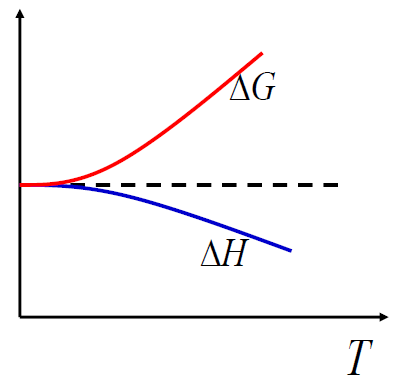
\includegraphics[width=0.4\textwidth]{third_law_nernst.png}
\caption{能斯特假设：$\Delta G$ 与 $\Delta H$ 在 $T\to 0$ 时趋于一致（需插入原PPT第18次课第21页图片）}
\label{fig:nernst}
\end{figure}

这意味着
\begin{equation}
\lim_{T\to 0}\left(\frac{\partial\Delta G}{\partial T}\right)_p = 0,\qquad
\lim_{T\to 0}\left(\frac{\partial\Delta H}{\partial T}\right)_p = 0.
\end{equation}
由于 $\displaystyle\left(\frac{\partial G}{\partial T}\right)_p = -S$，故
\begin{equation}
\lim_{T\to 0}\Delta S = 0.
\end{equation}


% --------------------------------------------
\subsubsection*{热力学第三定律的表述}
% --------------------------------------------

\paragraph{能斯特定理}

\textbf{能斯特定理}（热力学第三定律的早期表述）：系统的熵在等温过程中的改变随绝对温度趋于零，即
\begin{equation}
\boxed{\lim_{T\to 0}(\Delta S)_T = 0}
\end{equation}

\paragraph{普朗克假设}

1911年，普朗克（Planck）进一步假设：在绝对零度时，任何完美晶体的熵为零：
\begin{equation}
\boxed{\lim_{T\to 0} S(T) = 0}
\end{equation}
这样便为熵规定了绝对数值，无需再引入任意常数。

\paragraph{推论}

由热力学第三定律可推出以下重要结论：

\begin{itemize}
\item \textbf{热容趋于零}：$\displaystyle\lim_{T\to 0} C_V = 0,\quad \lim_{T\to 0} C_p = 0$。
\item \textbf{热膨胀停止}：$\displaystyle\lim_{T\to 0}\left(\frac{\partial V}{\partial T}\right)_p = 0$。
\item \textbf{没有气体在绝对零度仍保持理想气体行为}。
\item \textbf{绝对零度不可达}：不可能通过任何有限的过程把一个物体冷却到绝对零度。
\end{itemize}

\begin{remark}
热力学第三定律与量子力学密切相关。在绝对零度时，完美晶体处于唯一的基态，其微观状态数 $\Omega=1$，由玻尔兹曼熵 $S=k_B\ln\Omega$ 直接得到 $S=0$。
\end{remark}

\newpage
% ============================================
\section{第六章：液体}
% ============================================

\subsection{液体的性质}

\subsubsection*{液体的定义与特征}

\textbf{液体}：具有一定体积、没有弹性（没有切变模量）、没有一定形状、不易被压缩的可流动物体。

\subsubsection*{液体的分类}

按分子间不同的作用力，液体可分为：
\begin{itemize}
    \item \textbf{范德瓦尔斯液体}：分子不具有电偶极矩，如液态惰性气体（氦除外）、液态氢；
    \item \textbf{极性液体}：分子具有较大的电偶极矩，如氯化氢液体、溴化氢液体；
    \item \textbf{缔合性液体}：分子间有很强的吸引作用，结构较稳固，黏滞性大，如水、甘油；
    \item \textbf{金属液体}：存在自由电子，传热、导电性能较好，如金属熔解形成的液体；
    \item \textbf{量子液体}：黏滞性消失，呈超流态等量子现象，如液氦（$^4$He）II；
    \item \textbf{液晶}：介于固态与液态之间的过渡状态（在一定温度区间内），力学性质——具有流动性；光学性质——各向异性。
\end{itemize}


\subsection{液体的微观结构及研究方法}

\subsubsection*{微观结构特征}

液体分子的排列方式：\textbf{短程有序、长程无序}。

\begin{figure}[htbp]
\centering
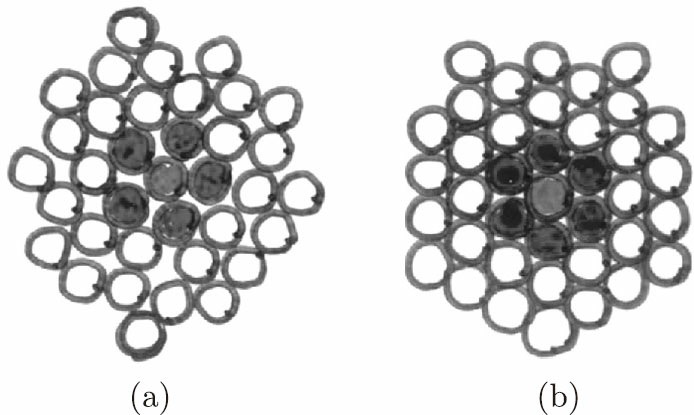
\includegraphics[width=0.35\textwidth]{liquid_structure.png}
\caption{液体与固体（晶体）的结构对比示意图（需插入原PPT第19次课第1页图片）}
\label{fig:liquid_structure}
\end{figure}

利用X射线衍射方法可测量液体的径向分布函数。实验表明，液体的排列方式随温度变化：温度升高，有序性降低，逐渐接近气态。

\subsubsection*{径向分布函数}

\textbf{径向分布函数} $g(r)$：以任意粒子的质心为中心，画出不同半径的一系列同心球面，两个相邻球面所决定的球壳体积相等，而球壳的厚度又足够小，每个球壳中的平均粒子数分布称为径向分布函数。$g(r)$ 为相距参考粒子 $r$ 处粒子的密度。

\begin{figure}[htbp]
\centering
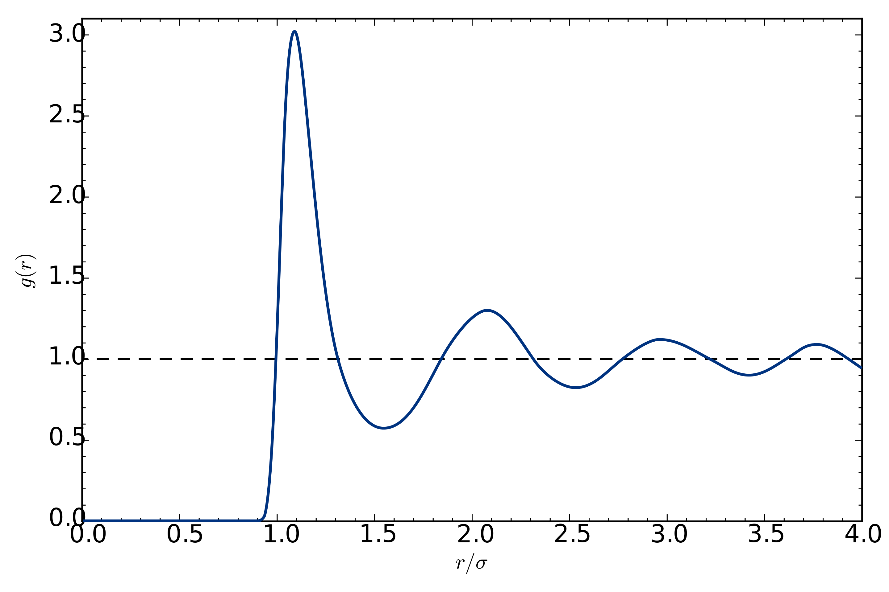
\includegraphics[width=0.4\textwidth]{radial_distribution.png}
\caption{径向分布函数示意图及液态氩的实验测量结果（需插入原PPT第19次课第1--2页图片）}
\label{fig:radial_dist}
\end{figure}

\subsubsection*{液体分子的热运动}

\textbf{热运动模式}：仅在其平衡位置附近作振动。

\textbf{热运动特点}：同一单元中液体分子的振动方向基本一致，不同单元中液体分子的振动方向各不相同。

\textbf{振动中心及相应振动时间不定}。液体分子在各个平衡位置振动时间的平均值为
\begin{equation}
\bar{\tau} = \bar{\tau}_0 e^{E_a/k_BT},
\end{equation}
其中 $E_a$ 为激活能。通常分子在一个单元平均振动 $10^2\sim10^3$ 次。

\begin{figure}[htbp]
\centering
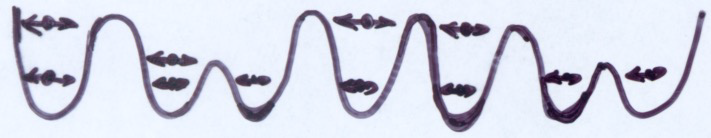
\includegraphics[width=0.4\textwidth]{liquid_vibration.png}
\caption{液体分子在平衡位置附近振动的势阱模型（需插入原PPT第19次课第3页图片）}
\label{fig:liquid_vib}
\end{figure}

\subsubsection*{液体的研究方法}

\begin{itemize}
    \item \textbf{视为无序系统}，类似较``稠密''的气体；在临界点以上，气体和液体没有明显的区别。
    \item \textbf{视为高温的无序固体}（无序固体）：
    \begin{itemize}
        \item 三相点附近液体的内能等性质接近固体（但在临界点接近气体）；
        \item 固体熔解前后定压热容接近液体；
        \item 液体的密度接近固体（$85\%\sim90\%$），可以把液体看成是间隙增加 $10\%\sim15\%$ 的不完美固体。
    \end{itemize}
    \item \textbf{径向分布函数法}。
\end{itemize}

\begin{figure}[htbp]
\centering
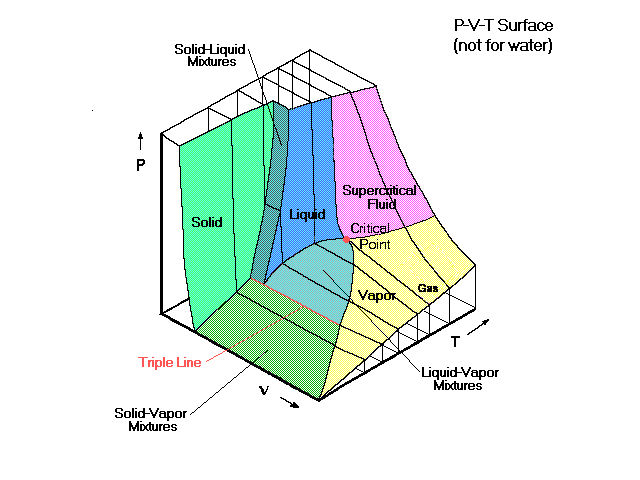
\includegraphics[width=0.35\textwidth]{pvt_surface.png}
\caption{物质的状态方程 $p$-$V$-$T$ 曲面（示意）（需插入原PPT第19次课第3页图片）}
\label{fig:pvt_surface}
\end{figure}


\subsection{液体的热容量}

实验表明，液体的定压热容与固体的相近：
\begin{equation}
C_p^{(L)} \approx C_p^{(S)}.
\end{equation}

由杜隆--珀替定律，摩尔定压热容
\begin{equation}
C_{p,m}^{(L)} \approx 3R.
\end{equation}

\textbf{与温度的关系}：
\begin{itemize}
    \item 一般随 $T$ 升高而增大，如乙醚等；有些反而减少，如液态铅；
    \item 少数不单调，如水：
    \begin{center}
    $0^\circ\mathrm{C}\to 75.98$,\quad $35^\circ\mathrm{C}\to 75.27$,\quad $100^\circ\mathrm{C}\to 75.95$ \quad（单位：$\mathrm{J/(mol\cdot K)}$）
    \end{center}
\end{itemize}

对固体有 $C_V^{(S)} \approx C_p^{(S)}$；但对液体 $C_V^{(L)} \neq C_p^{(L)}$，且 $C_p^{(L)}-C_V^{(L)} \neq \text{常数}$。

对任意系统，由 $H=U+pV$ 及多元复合函数的偏导数，有
\begin{equation}
\left(\frac{\partial H}{\partial T}\right)_p = \left(\frac{\partial U}{\partial T}\right)_V + \left[p+\left(\frac{\partial U}{\partial V}\right)_T\right]\left(\frac{\partial V}{\partial T}\right)_p.
\end{equation}

利用内能方程 $\displaystyle\left(\frac{\partial U}{\partial V}\right)_T = T\left(\frac{\partial p}{\partial T}\right)_V - p$，得
\begin{equation}
\boxed{C_p - C_V = \left[p+\left(\frac{\partial U}{\partial V}\right)_T\right]\left(\frac{\partial V}{\partial T}\right)_p = T\left(\frac{\partial p}{\partial T}\right)_V\left(\frac{\partial V}{\partial T}\right)_p.}
\end{equation}

又可写为
\begin{equation}
C_p - C_V = T\left(\frac{\partial p}{\partial T}\right)_{V,N}\left(\frac{\partial V}{\partial T}\right)_{p,N}
= TV\frac{\alpha^2}{\kappa_T},
\end{equation}
其中 $\alpha$ 为体膨胀系数，$\kappa_T$ 为等温压缩系数。

\begin{figure}[htbp]
\centering
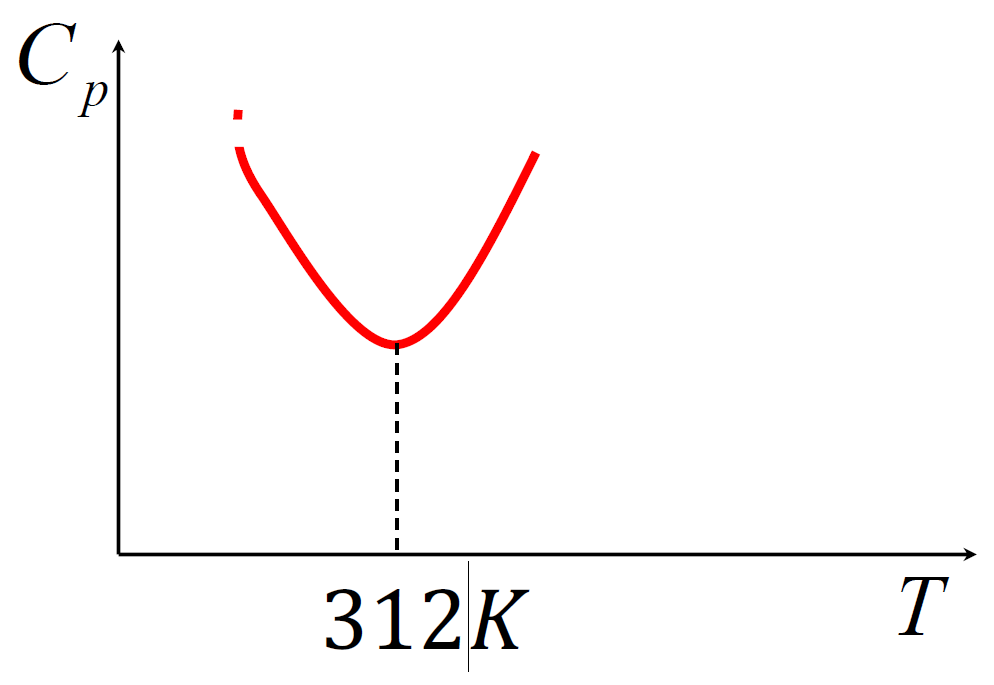
\includegraphics[width=0.3\textwidth]{liquid_heat_capacity.png}
\caption{液体热容随温度变化示意图（需插入原PPT第19次课第4页图片）}
\label{fig:liquid_cp}
\end{figure}


\subsection{液体的可压缩性和热膨胀}

\subsubsection*{压缩性质}

液体很难被压缩，等温压缩系数定义为
\begin{equation}
\kappa = -\frac{1}{V}\left(\frac{\partial V}{\partial p}\right)_T.
\end{equation}

液体的等温压缩系数比固体的稍大：
\begin{equation}
\kappa_L \sim 10^{-5}\,\mathrm{atm^{-1}},\qquad \kappa_S \sim 10^{-6}\,\mathrm{atm^{-1}}.
\end{equation}
可用 van de Waals 模型近似。

\subsubsection*{热膨胀性质}

体膨胀系数
\begin{equation}
\alpha = \frac{1}{V}\left(\frac{\partial V}{\partial T}\right)_p.
\end{equation}

体膨胀系数一般比固体的大，但个别的较小。例如室温下：
\begin{equation}
\mathrm{H_2O}:\ 1.8\times10^{-4}\,\mathrm{K^{-1}};\qquad \mathrm{Cu}:\ 5\times10^{-3}\,\mathrm{K^{-1}}.
\end{equation}

\textbf{水在 $0$ 至 $4$ 摄氏度间的反常膨胀}。

\begin{figure}[htbp]
\centering
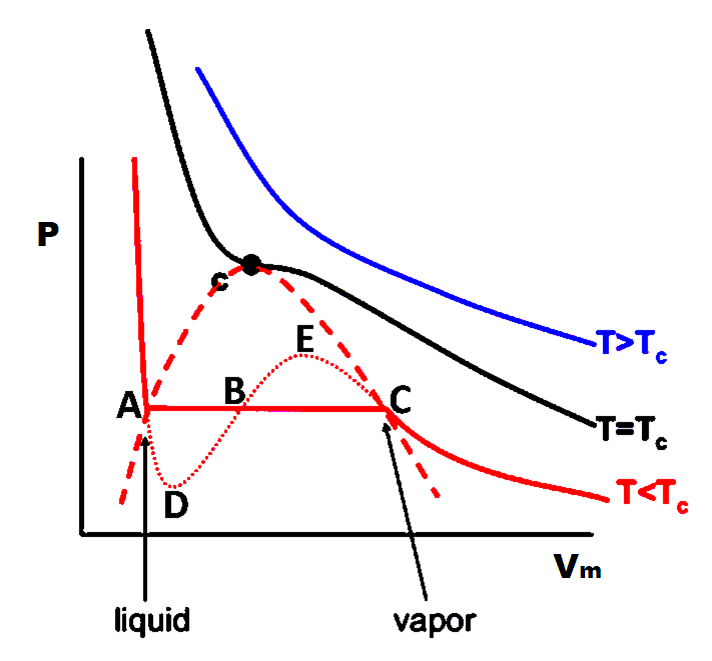
\includegraphics[width=0.35\textwidth]{liquid_compressibility.png}
\caption{液体的 $p$-$V$ 等温线及气液共存区（需插入原PPT第19次课第5页图片）}
\label{fig:liquid_pv}
\end{figure}


\subsection{液体的输运性质}

\subsubsection*{黏滞性（动量输运）}

\textbf{黏度与温度的关系}：\textbf{温度越低，黏度越大}。

\textbf{物理根源}：流动性取决于定居时间，黏滞性起因于两层分子间的吸引作用。定居时间越长，流动性越低，黏度越大。

费朗克尔--安德逊公式：
\begin{equation}
\bar{\tau} = \bar{\tau}_0 e^{E_a/k_BT}
\quad\Rightarrow\quad
\eta = \eta_0 e^{E_a/k_BT}.
\end{equation}

与气体相比，气体黏度
\begin{equation}
\eta = \frac{2\alpha_\eta}{3\sigma}\sqrt{\frac{mk_BT}{\pi}} \propto T^{1/2}
\quad\left(\text{简版 }\eta = \frac{1}{3}\bar{v}\bar{\lambda}\rho\right),
\end{equation}
即气体黏度随温度升高而增大，与液体相反。

\subsubsection*{热传导（能量输运）}

一般液体的导热性很差；金属液体的导热性相当好。

\textbf{物理根源}：
\begin{itemize}
    \item 一般液体热传导过程中能量传递主要通过定域分子间的碰撞，不同区域间分子的运动占次要地位，导热机理与固体相似；
    \item 金属液体热传导过程中能量传递主要通过自由电子的热运动，定域分子间的碰撞占次要地位，导热机理与气体导热相似。
\end{itemize}

气体热导率
\begin{equation}
\kappa = \frac{2\alpha_\kappa C_V}{3\sigma}\sqrt{\frac{mk_BT}{\pi}} \propto T^{1/2}.
\end{equation}

\begin{center}
\begin{tabular}{c|c|c|c|c|c}
\hline
物质 & 水($20^\circ\mathrm{C}$) & 氢($16\,\mathrm{K}$) & 氧($80\,\mathrm{K}$) & 汞($0^\circ\mathrm{C}$) & 铅($350^\circ\mathrm{C}$) \\
\hline
$\kappa\ (\mathrm{J/(m\cdot s\cdot K)})$ & 0.597 & 0.109 & 0.163 & 25.31 & 16.0 \\
\hline
\end{tabular}
\end{center}

\subsubsection*{扩散（质量输运）}

\textbf{扩散方式}：跳跃式。以 $x$ 方向为例，对研究对象分子 O，它需要克服分子 r、s、t、u 的吸引力，并推开分子 p、q 后，才能穿出单元边界。之后 p、q 闭合，O 分子在新的位置上与其它分子组成新的单元。

\textbf{扩散系数与温度的关系}：
\begin{equation}
D \propto \frac{1}{\bar{\tau}}
\quad\Rightarrow\quad
D = D_0 e^{-E_a/k_BT}.
\end{equation}

气体扩散系数 $D \propto T^{1.5}$。

液体扩散与固体填隙原子扩散类似，不同于气体。

\begin{figure}[htbp]
\centering
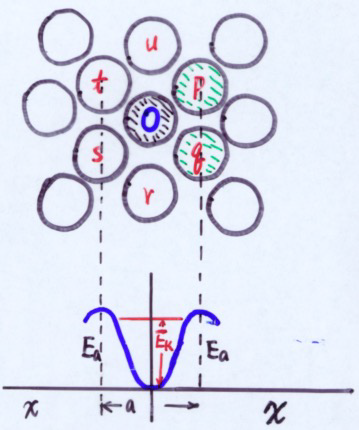
\includegraphics[width=0.4\textwidth]{liquid_diffusion.png}
\caption{液体分子扩散的跳跃机制示意图（需插入原PPT第19次课第6页图片）}
\label{fig:liquid_diff}
\end{figure}


\subsection{液体的表面性质}

\subsubsection*{表面与表面张力}

\textbf{表面}：液体与自己的蒸汽或另一种介质接触的交界面称为液体表面。

\textbf{表现现象}：各种液滴；水面上可以承受硬币、钢针等物体；金属框内的细线在有无液面时呈不同的形状。

\textbf{表面张力}：在液体表面上想象画一条线，该线两侧的液面相互存在着拉力作用。这个位于液面内处处与此线垂直的拉力称为表面张力。

\begin{figure}[htbp]
\centering
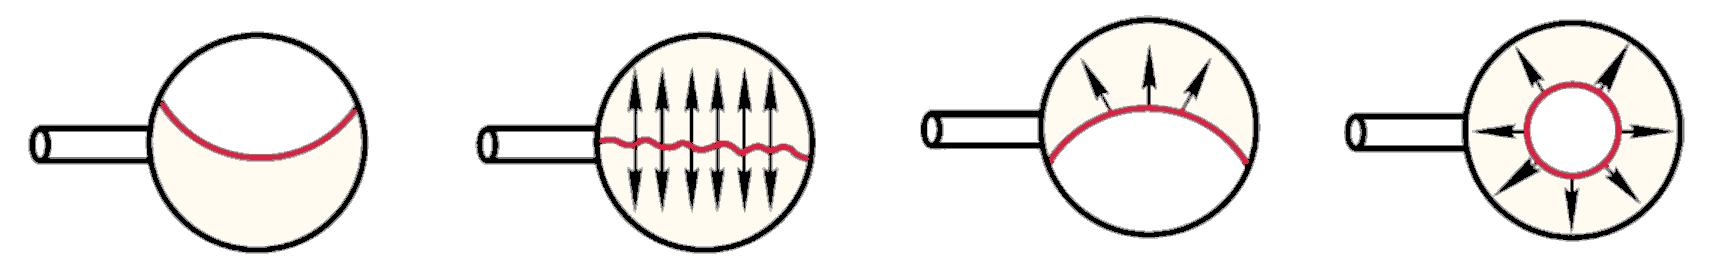
\includegraphics[width=0.7\textwidth]{surface_tension_demo.png}
\caption{表面张力的表现现象（需插入原PPT第19次课第7页图片）}
\label{fig:surface_demo}
\end{figure}

\subsubsection*{表面张力的性质}

\begin{itemize}
    \item 与表面积的大小无关；
    \item \textbf{物理根源}：表面层内分子之间的相互作用。
\end{itemize}

设分子间引力的有效半径为 $R$。因为分子之间的作用为短程作用，一个分子只受以它为中心、以 $R$ 为半径的球内的分子的作用，该球称为\textbf{分子作用球}。在液体内部，分子作用球完整，每个分子所受的合力为 $0$。在表面，分子作用球不完整，因为少了球冠部分，从而分子所受合力不为 $0$，而是垂直于表面的一个力（指向液体内部）。

\begin{figure}[htbp]
\centering
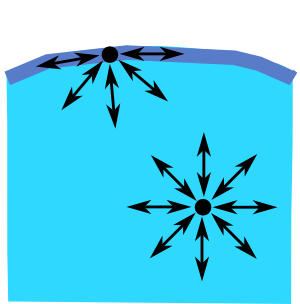
\includegraphics[width=0.35\textwidth]{molecular_sphere.png}
\caption{液体表面层与内部的分子作用球（需插入原PPT第19次课第7页图片）}
\label{fig:mol_sphere}
\end{figure}

\subsubsection*{表面张力系数——力}

由于表面层（厚度为分子作用球半径）内分子分布\textbf{各向同性}被破坏，在液面上长为 $\Delta l$ 的线出现表面张力 $f$，其方向恒与 $\Delta l$ 垂直，大小与 $\Delta l$ 成正比，即
\begin{equation}
f = \alpha\Delta l,\qquad [\alpha] = \mathrm{N\,m^{-1}}.
\end{equation}

\textbf{表面张力系数}：单位长度的直线两侧液面的相互拉力。

\subsubsection*{表面张力系数——功}

外力作用，表面积扩大的过程：外力作功为
\begin{equation}
\mathrm{d}W = f\,\mathrm{d}x = \alpha\cdot 2l\,\mathrm{d}x = \alpha\,\mathrm{d}A_s,
\end{equation}
其中 $\mathrm{d}A_s = 2l\,\mathrm{d}x$ 为液面增加的表面积（注意薄膜有两个表面）。

于是
\begin{equation}
\boxed{\alpha = \frac{\mathrm{d}W}{\mathrm{d}A_s}}
\end{equation}
即液面改变单位面积外界所作的功（等温、等体）。

\begin{figure}[htbp]
\centering
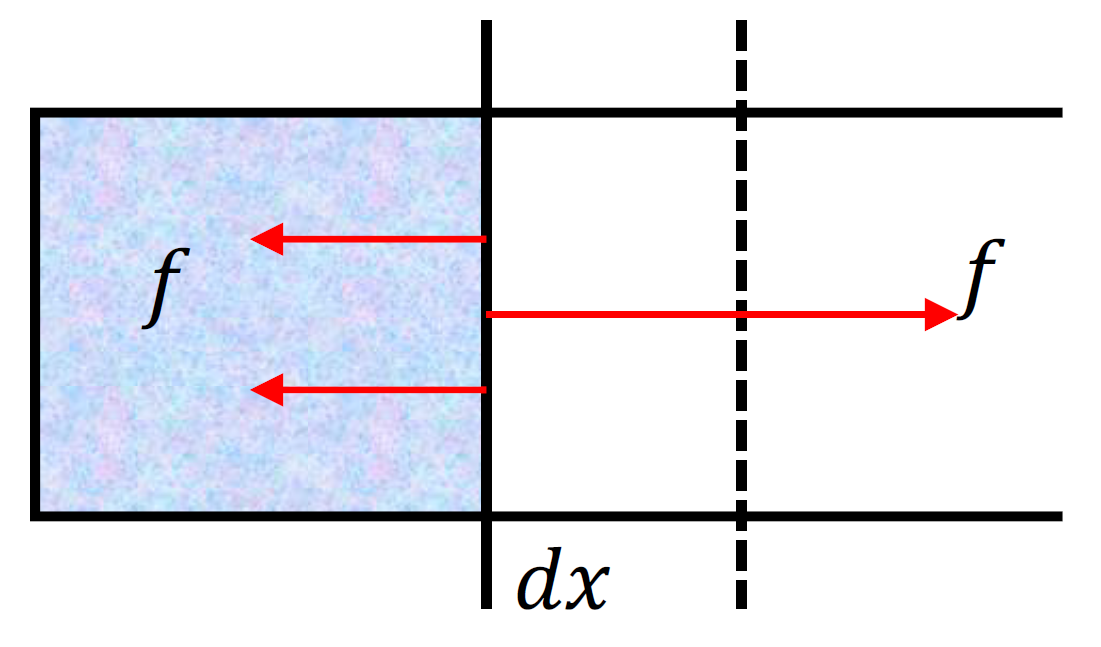
\includegraphics[width=0.3\textwidth]{surface_work.png}
\caption{表面张力系数与外力做功（需插入原PPT第19次课第8页图片）}
\label{fig:surface_work}
\end{figure}

\subsubsection*{表面张力的微观解释}

设一个分子平均有 $s$ 个近邻分子（即 $s$ 条键），每对分子键能 $\Delta\varepsilon$，平均每个分子键能为 $\dfrac{1}{2}s\Delta\varepsilon$；设表面分子平均有 $\eta s$ 条键，则表面层中分子的键能为 $\dfrac{1}{2}\eta s\Delta\varepsilon$；表面层内外分子键能差为 $\dfrac{1}{2}(1-\eta)s\Delta\varepsilon$。设面积为 $\mathrm{d}A_s$ 的表面层中有 $N_s$ 个液体分子，则
\begin{equation}
\mathrm{d}W = \frac{1}{2}(1-\eta)s\Delta\varepsilon\,N_s = \alpha\,\mathrm{d}A_s
\quad\Rightarrow\quad
\alpha = \frac{1}{2}\frac{(1-\eta)s\Delta\varepsilon\,N_s}{\mathrm{d}A_s}.
\end{equation}

摩尔汽化热为 $\displaystyle\Lambda_m = \frac{1}{2}N_A s\Delta\varepsilon$，单位面积的表面层粒子数 $\displaystyle z = \frac{N_s}{\mathrm{d}A_s}$，代入得
\begin{equation}
\alpha = \frac{(1-\eta)\Lambda_m z}{N_A}.
\end{equation}

设粒子的直径为 $d$，每个表面粒子占有的表面积近似为
\begin{equation}
d^2 = \frac{\mathrm{d}A_s}{N_s} = \frac{1}{z},\qquad
d^3 N_A = \frac{\mu}{\rho}
\quad\Rightarrow\quad
d^2 = \left(\frac{\mu}{\rho N_A}\right)^{2/3}.
\end{equation}

于是
\begin{equation}
\alpha = \frac{(1-\eta)\Lambda_m z}{N_A}
= \frac{(1-\eta)\Lambda_m}{N_A d^2}
= (1-\eta)\frac{\Lambda_m}{N_A}\left(\frac{\rho N_A}{\mu}\right)^{2/3}.
\end{equation}

对大多数液体，$\eta \approx 0.7$。计算值与实验值对比如下：
\begin{equation*}
\text{计算}\begin{cases}
\alpha(\mathrm{Ar}) = 0.013\,\mathrm{J\,m^{-2}}\\
\alpha(\mathrm{Ne}) = 0.0055\,\mathrm{J\,m^{-2}}
\end{cases}
\qquad
\text{实验}\begin{cases}
\alpha(\mathrm{Ar}) = 0.014\,\mathrm{J\,m^{-2}}\\
\alpha(\mathrm{Ne}) = 0.004\,\mathrm{J\,m^{-2}}
\end{cases}
\end{equation*}

\subsubsection*{表面张力系数与温度的关系}

表面张力（表面张力系数）与面积无关，仅与温度等条件有关。并且，\textbf{表面张力系数随温度升高而降低}，即
\begin{equation}
\frac{\partial\alpha}{\partial T} = \frac{1-\eta}{N_A^{1/3}}\frac{\mathrm{d}\Lambda_m}{\mathrm{d}T}\left(\frac{\rho}{\mu}\right)^{2/3} < 0.
\end{equation}

\textbf{物理解释}：
\begin{itemize}
    \item 液体通常都具有热胀冷缩的性质，温度升高，分子间距通常会增大，摩尔汽化热减小；
    \item 从力的方面考虑：分子间距离增大，导致吸引力减小，所以表面张力减小。
\end{itemize}

\subsubsection*{影响表面张力系数的其他因素}

\begin{itemize}
    \item \textbf{液体的密度等内禀性质}：
    \begin{equation}
    \alpha = (1-\eta)\frac{\Lambda_m}{N_A}\left(\frac{\rho N_A}{\mu}\right)^{2/3}.
    \end{equation}
    
    \item \textbf{液面外相邻物质的性质}：常见液体水和汞在其外侧具有不同相邻物质情况下的表面张力系数不同。
    
    \begin{center}
    \begin{tabular}{c|ccc|c|c|c}
    \hline
    液体--相邻物质 & \multicolumn{3}{c|}{水--空气} & 水--苯 & 汞--真空 & 汞--水 \\
    \hline
    温度$/^\circ\mathrm{C}$ & 10 & 30 & 50 & 20 & 0 & 20 \\
    表面张力系数$/10^{-3}\,\mathrm{N\,m^{-1}}$ & 74.22 & 71.18 & 67.91 & 33.6 & 480 & 472 \\
    \hline
    \end{tabular}
    \end{center}
    
    \item \textbf{液体中的杂质}：有的使表面张力系数增大，有的使表面张力系数减小。使表面张力系数减小的物质称为\textbf{表面活性物质}，例如醇、酸、醛、酮等。
\end{itemize}

\subsubsection*{表面能（表面自由能）}

外力克服表面层中分子力的合力所作的功等于表面层中的分子引力势能的增加，这种增加的分子势能称为\textbf{表面自由能}，简称\textbf{表面能}。

等温条件下
\begin{equation}
\mathrm{d}W = \alpha\,\mathrm{d}A_s = \mathrm{d}(U-TS) = \mathrm{d}F,
\end{equation}
得
\begin{equation}
\alpha = \left(\frac{\partial F_s}{\partial A_s}\right)_T.
\end{equation}

若表面为两种不同种类液体的接触面，两种液体各有一个表面层。设分子力较弱的液体为 B，较强的为 A，则液体 A 的表面层中分子吸引力的合力仍垂直向下，表面能为正。液体 B 的表面层中分子吸引力的合力也垂直向下，其中的分子欲进入液体 B 的内部，也需要克服该垂直向下的力。所以，\textbf{液体 B 的表面能为负}。

\subsubsection*{表面自由能和表面内能}

表面自由能 $F_s$ 为等温条件下外力在扩展表面时所作的功；但是 $F_s$ \textbf{不是}表面内能，表面内能需要具体确定。

由 $U=F+TS$，$F_s=\alpha A_s$，得表面内能
\begin{equation}
U_s = F_s + TS = \alpha A_s + TS.
\end{equation}

又
\begin{equation}
\mathrm{d}F_s = \mathrm{d}U_s - T\,\mathrm{d}S - S\,\mathrm{d}T.
\end{equation}

由热力学第一定律
\begin{equation}
\mathrm{d}U_s = \mathrm{d}Q + \mathrm{d}W = T\,\mathrm{d}S + \alpha\,\mathrm{d}A_s,
\end{equation}
故
\begin{equation}
\mathrm{d}F_s = \alpha\,\mathrm{d}A_s - S\,\mathrm{d}T.
\end{equation}

对于表面，$F_s = F_s(A_s,T) = \alpha A_s$，其全微分
\begin{equation}
\mathrm{d}F_s = \left(\frac{\partial F_s}{\partial A_s}\right)_T\mathrm{d}A_s + \left(\frac{\partial F_s}{\partial T}\right)_{A_s}\mathrm{d}T
= \alpha\,\mathrm{d}A_s + A_s\left(\frac{\partial\alpha}{\partial T}\right)_{A_s}\mathrm{d}T.
\end{equation}

比较两式，得
\begin{equation}
S = -\left(\frac{\partial\alpha}{\partial T}\right)_{A_s}A_s.
\end{equation}

于是\textbf{表面内能}
\begin{equation}
\boxed{U_s = \alpha A_s - TA_s\left(\frac{\partial\alpha}{\partial T}\right)_{A_s}}
\end{equation}

\textbf{表面内能密度}
\begin{equation}
\boxed{u_s = \alpha - T\left(\frac{\partial\alpha}{\partial T}\right)_{A_s}}
\end{equation}

\subsubsection*{例题：油滴分散}

\textbf{题目}：水--油界面表面张力系数为 $\alpha=0.018\,\mathrm{N/m}$。为了使一个 $1\,\mathrm{g}$ 的大油滴在水内等温地散布成半径为 $r=10\,\mu\mathrm{m}$ 的小油滴，需作功多少？（油密度 $\rho=900\,\mathrm{kg/m^3}$）

\textbf{解}：由表面张力的物理起因知，大油滴散布成大量小油滴时，与油滴相邻的水的表面自由能的增量等于外力所作的功，即有
\begin{equation}
\Delta W = \Delta F = \alpha\Delta A_s,
\end{equation}
其中 $\Delta A_s$ 是与油滴相邻的水的表面积的增量，即油滴表面积的增量。设大油滴的半径为 $R$，分裂成 $N$ 个小油滴，则
\begin{equation}
\Delta A_s = 4\pi(Nr^2 - R^2).
\end{equation}

因油的质量不变，有
\begin{equation}
m = \frac{4}{3}\pi R^3\rho = \frac{4}{3}N\pi r^3\rho
\quad\Rightarrow\quad
R^2 = N^{2/3}r^2.
\end{equation}

于是
\begin{equation}
\Delta A_s = 4\pi N^{2/3}r^2(N^{1/3}-1) \approx 4\pi r^2 N
= 4\pi r^2\frac{m}{\frac{4}{3}\pi r^3\rho}
= \frac{3m}{r\rho}.
\end{equation}

故
\begin{equation}
\boxed{\Delta W = \alpha\Delta A_s = \frac{3\alpha m}{r\rho}
= \frac{3\times0.018\times1\times10^{-3}}{10\times10^{-6}\times900}
= 6\times10^{-3}\,\mathrm{J}}
\end{equation}

% --------------------------------------------
\subsubsection*{弯曲液面内外压强差}
% --------------------------------------------

任意弯曲液面内外的压强差都可以表示为
\begin{equation}
\boxed{\Delta p = p_i - p_o = \alpha\left(\frac{1}{R_1}+\frac{1}{R_2}\right)}
\end{equation}
此即\textbf{拉普拉斯公式}（Laplace formula）。

其中 $R_1$、$R_2$ 为过弯曲液面上一点的一对相互垂直正截口的曲率半径。
\begin{itemize}
    \item 曲率中心在液体内 $R>0$，液体外 $R<<0$；
    \item \textbf{正截口}：包含曲面法线的平面与曲面的交线。
\end{itemize}

\begin{figure}[htbp]
\centering
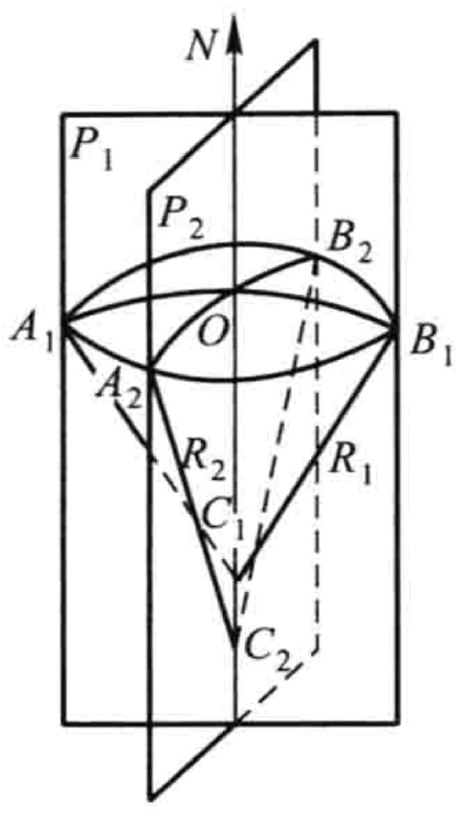
\includegraphics[width=0.35\textwidth]{laplace_pressure.png}
\caption{弯曲液面曲率半径与正截口示意图（需插入原PPT第20次课第2页图片）}
\label{fig:laplace}
\end{figure}

\paragraph{证明}

一个液面系统包括内部、表面层、外界三部分，分别记之为 $i$、$\gamma$、$o$。由平衡态的自由能判据
\begin{equation}
\delta F_i + \delta F_\gamma + \delta F_o = 0.
\end{equation}

各部分功的变分：
\begin{align}
\delta F_i &= \delta W_i = -p_i\,\delta V_i,\\
\delta F_\gamma &= \delta W_\gamma = \alpha\,\delta A_s,\\
\delta F_o &= \delta W_o = -p_o\,\delta V_o.
\end{align}

$\gamma$ 部分体积可忽略，$\delta V_i = -\delta V_o$，代入得
\begin{equation}
-p_i\,\delta V_i + \alpha\,\delta A_s - p_o\,\delta V_o = 0
\quad\Rightarrow\quad
p_i - p_o = \alpha\frac{\delta A_s}{\delta V_i}.
\end{equation}

如图，面积元 $A_s = ab\times cd = R_1\,\mathrm{d}\varphi_1 \times R_2\,\mathrm{d}\varphi_2$。设表面在内外压强差作用下有小位移 $\mathrm{d}\xi$，则
\begin{align}
\delta A_s &= (R_2+\mathrm{d}\xi)\,\mathrm{d}\varphi_2\cdot(R_1+\mathrm{d}\xi)\,\mathrm{d}\varphi_1 - R_1R_2\,\mathrm{d}\varphi_1\mathrm{d}\varphi_2 \notag\\
&\approx \mathrm{d}\xi\,(R_1+R_2)\,\mathrm{d}\varphi_1\mathrm{d}\varphi_2
= \left(\frac{1}{R_1}+\frac{1}{R_2}\right)\mathrm{d}\xi\,A_s
= \left(\frac{1}{R_1}+\frac{1}{R_2}\right)\delta V_\gamma.
\end{align}

于是
\begin{equation}
\frac{\delta A_s}{\delta V_i} = \frac{1}{R_1}+\frac{1}{R_2},
\end{equation}
代入即得拉普拉斯公式。

\paragraph{简单讨论}

\begin{itemize}
\item \textbf{球形液面}：$R_1=R_2=R$，则
\begin{equation}
\Delta p = p_i - p_o = \frac{2\alpha}{R}.
\end{equation}

\item \textbf{柱形液面}：$R_1=R,\ R_2=\infty$，则
\begin{equation}
\Delta p = p_i - p_o = \frac{\alpha}{R}.
\end{equation}
\end{itemize}

液面形状由其内部、外部及表面三部分的平衡所决定。

\begin{figure}[htbp]
\centering
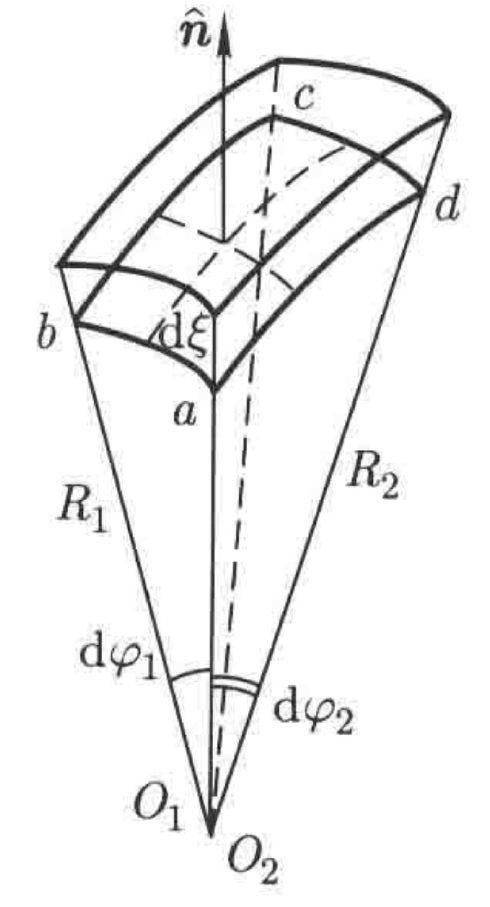
\includegraphics[width=0.5\textwidth]{surface_shapes.png}
\caption{液面凸与液面凹的压强分布示意（需插入原PPT第20次课第3页图片）}
\label{fig:surface_shapes}
\end{figure}

\subsubsection*{拉普拉斯公式的实验检验}

实验装置如图所示：两个连通的不同半径的肥皂泡。

\begin{figure}[htbp]
\centering
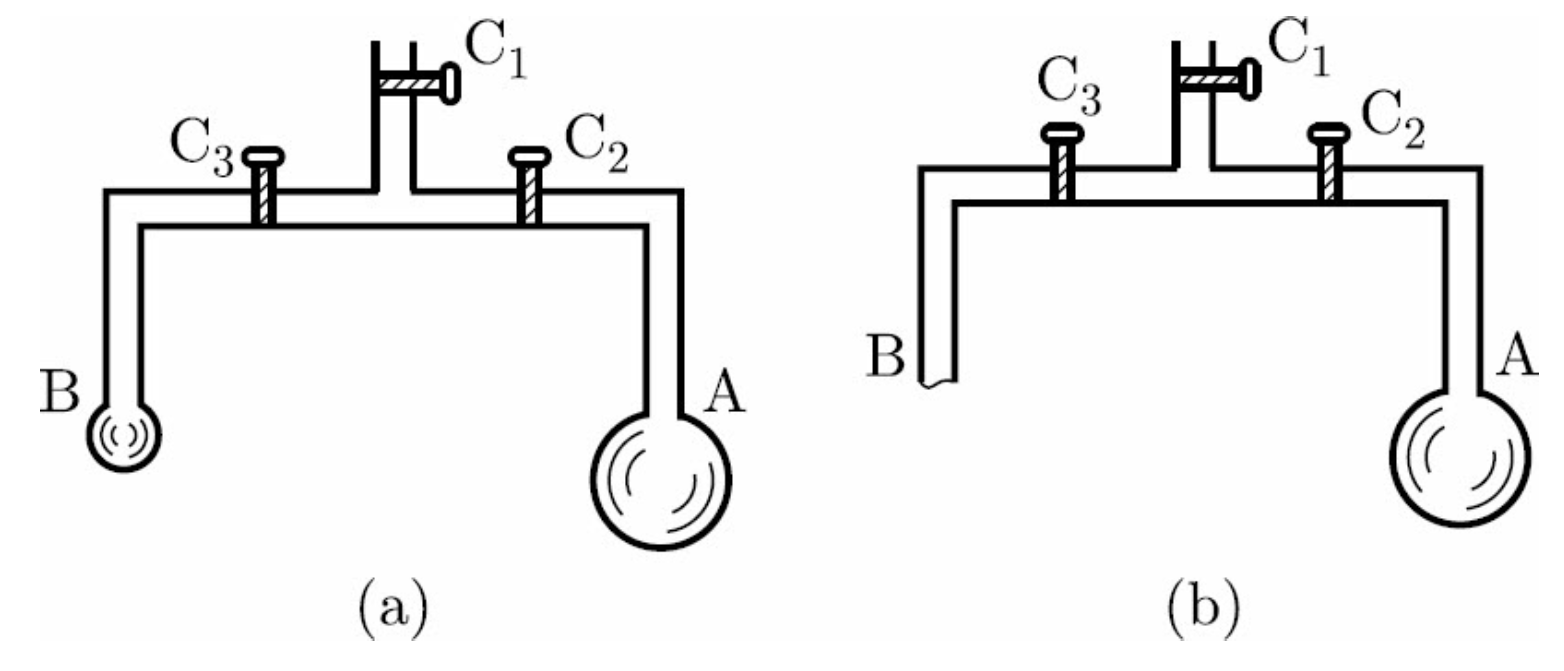
\includegraphics[width=0.5\textwidth]{soap_bubble_experiment.png}
\caption{连通肥皂泡实验：验证拉普拉斯公式（需插入原PPT第20次课第3页图片）}
\label{fig:soap_bubble}
\end{figure}

\textbf{实验现象}：肥皂泡 A（半径较大）越来越大，肥皂泡 B（半径较小）越来越小。

\textbf{结论}：说明肥皂泡 A 中的气体压强小于肥皂泡 B 中的气体压强，与拉普拉斯公式 $p-p_0=4\alpha/r$（肥皂泡有内外两个表面，故为 $4\alpha/r$）一致：半径越小，内外压强差越大。

\subsubsection*{例题：吹肥皂泡}

\textbf{题目}：将空气等温地压缩进肥皂泡内，最后吹成半径为 $r=2.5\,\mathrm{cm}$ 的肥皂泡。设肥皂水的表面张力系数为 $\alpha=0.044\,\mathrm{N/m}$，试求吹成此肥皂泡过程中应作多少功？

\textbf{解}：此过程可分为两部分：液体部分（等温等体，表面积增加）；气体部分（体积变化）。

设此过程可逆。肥皂泡半径为 $r$，泡内气体的压强为 $p$，体积为 $V$，温度为 $T$，大气压强为 $p_0$。肥皂泡有内外两个液膜表面，由弯曲液面内外压强差：
\begin{equation}
\Delta p = p_i - p_o = \frac{2\alpha}{r}\quad(\text{单个表面}),
\end{equation}
故泡内气体压强
\begin{equation}
p = p_0 + \frac{4\alpha}{r}.
\end{equation}

外界所作总功等于系统自由能增量：
\begin{equation}
\Delta W = \Delta U - T\Delta S = \Delta F = \Delta F_s + \Delta F_g.
\end{equation}

\textbf{表面自由能增量}（双层膜，内外两个表面）：
\begin{equation}
\Delta F_s = \alpha\cdot\Delta A_s = \alpha\cdot 8\pi r^2.
\end{equation}

\textbf{气体自由能增量}（等温压缩）：
\begin{equation}
\Delta F_g = -T_0\Delta S_G = \nu RT_0\ln\frac{p}{p_0}.
\end{equation}

于是
\begin{align}
\Delta W &= 8\pi\alpha r^2 + \nu RT_0\ln\frac{p}{p_0}
= 8\pi\alpha r^2 + \nu RT_0\ln\!\left(1+\frac{\Delta p}{p_0}\right) \notag\\
&\approx 8\pi\alpha r^2 + p_0V_0\cdot\frac{4\alpha}{p_0r}
= 8\pi\alpha r^2 + \frac{4\alpha}{r}\cdot\frac{4}{3}\pi r^3 \notag\\
&= 8\pi\alpha r^2 + \frac{16}{3}\pi\alpha r^2
= \frac{40}{3}\pi\alpha r^2.
\end{align}

代入数值：
\begin{equation}
\boxed{\Delta W = \frac{40}{3}\times3.14\times0.044\times(2.5\times10^{-2})^2
= 1.152\times10^{-3}\,\mathrm{J}}
\end{equation}


% ============================================
\subsection{润湿现象与毛细现象}
% ============================================

\subsubsection*{润湿现象}

如果液体可均匀附着于另一种液体或固体表面，则称之为\textbf{润湿现象}，或\textbf{浸润现象}；否则称之为\textbf{不润湿现象}，或\textbf{不浸润现象}。

\textbf{实例}：
\begin{itemize}
    \item 一种液体可在另一种液体（互不相溶）表面上形成一层薄膜，也可以形成液珠；
    \item 水能覆盖清洁的玻璃，但不能覆盖涂有油脂的玻璃，也不能覆盖整个荷叶；
    \item 水银不能覆盖整个玻璃，而只能在其上形成小珠。
\end{itemize}

\subsubsection*{接触角}

液固或液液接触处\textbf{液面的切线}与\textbf{液体内部两物质表面切线}之间的夹角称为这两种物质的\textbf{接触角}，记为 $\theta$。

\begin{figure}[htbp]
\centering
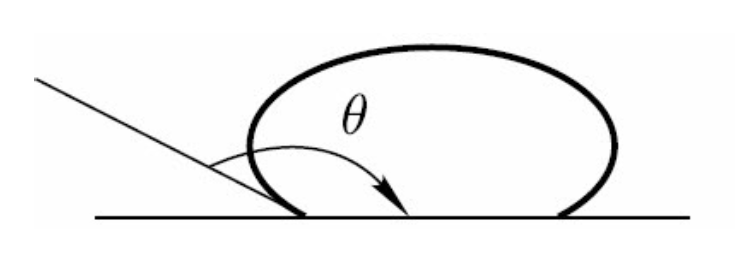
\includegraphics[width=0.35\textwidth]{contact_angle.png}
\caption{接触角定义与润湿程度的关系（需插入原PPT第20次课第4页图片）}
\label{fig:contact_angle}
\end{figure}

\textbf{润湿程度的度量}：接触角越小，润湿程度越高。
\begin{itemize}
    \item \textbf{完全润湿}：液体完全均匀地附着于另一种物质的表面；$\theta=0$；
    \item \textbf{部分润湿}：液体大致均匀地附着于另一种物质的表面，也称之为能润湿；$\theta\in(0,\pi/2)$；
    \item \textbf{部分不润湿}：介于完全不润湿和部分润湿之间的状态，也称之为不能润湿；$\theta\in(\pi/2,\pi)$；
    \item \textbf{完全不润湿}：液体处于另一种物质之上，但其间只有点接触；$\theta=\pi$。
\end{itemize}

\subsubsection*{液--液接触角的确定}

设 1、2 两种液体和空气 3 的交界为一圆环。图示为其纵切面，三种物质两两作用，整体平衡。

\begin{figure}[htbp]
\centering
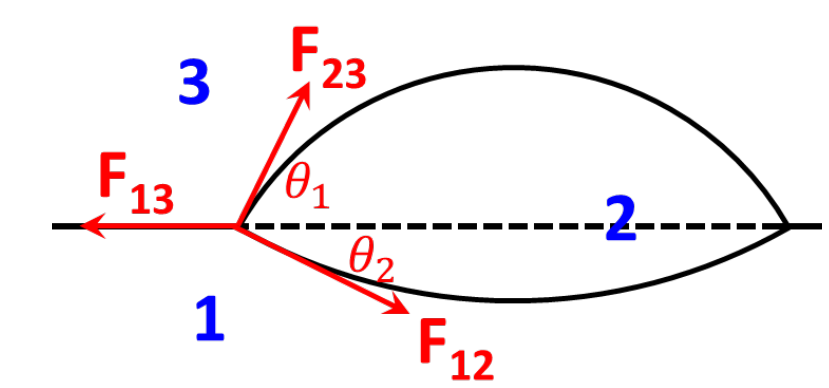
\includegraphics[width=0.35\textwidth]{liquid_liquid_contact.png}
\caption{液--液--气三相接触线的力学平衡（需插入原PPT第20次课第4页图片）}
\label{fig:ll_contact}
\end{figure}

在交界线上取线元 $\mathrm{d}l$，各界面张力分别为
\begin{equation}
f_{13}=\alpha_{13}\,\mathrm{d}l,\quad f_{23}=\alpha_{23}\,\mathrm{d}l,\quad f_{12}=\alpha_{12}\,\mathrm{d}l.
\end{equation}

力学平衡条件：
\begin{align}
\alpha_{13} &= \alpha_{23}\cos\theta_1 + \alpha_{12}\cos\theta_2 \quad (1)\\
0 &= \alpha_{23}\sin\theta_1 - \alpha_{12}\sin\theta_2 \quad\ \ (2)
\end{align}

令 $\Theta=\theta_1+\theta_2$，两式平方相加，得
\begin{equation}
\cos\Theta = \frac{\alpha_{13}^2-(\alpha_{12}^2+\alpha_{23}^2)}{2\alpha_{12}\alpha_{23}}.
\end{equation}

\subsubsection*{液--固界面上的接触角}

\begin{itemize}
    \item $\theta=\pi\ \Rightarrow$ 完全不润湿；
    \item $\theta\ge\pi/2\ \Rightarrow$ 不润湿；
    \item $\theta<\pi/2\ \Rightarrow$ 润湿；
    \item $\theta=0\ \Rightarrow$ 完全润湿。
\end{itemize}

\textbf{浸润现象的物理原因}：
\begin{itemize}
    \item \textbf{内聚力}：液体内的分子对表面层内液体分子的吸引力；
    \item \textbf{附着力}：固体内的分子对表面层内液体分子的吸引力。
\end{itemize}

内聚力与附着力的竞争决定液固界面的接触角：
\begin{itemize}
    \item 不浸润：内聚力大于附着力；
    \item 浸润：附着力大于内聚力。
\end{itemize}

\begin{figure}[htbp]
\centering
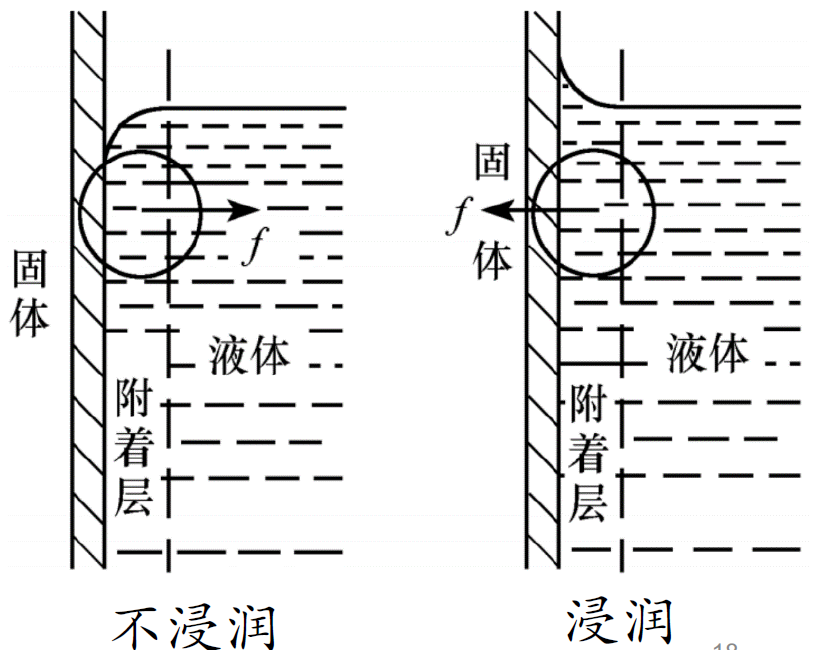
\includegraphics[width=0.5\textwidth]{wetting_mechanism.png}
\caption{浸润与不浸润的微观机制（需插入原PPT第20次课第5页图片）}
\label{fig:wetting_mech}
\end{figure}

\subsubsection*{液--固接触角的确定}

与液--液--气相似，但液体 1 变为固体（无变形），故 $\theta_2=0$，$\theta_1=\theta$。

由力学平衡条件（纵截面）：
\begin{equation}
F_{13}-F_{12}=F_{23}\cos\theta.
\end{equation}

由 $F_{13}=\alpha_{13}\,\mathrm{d}l,\ F_{12}=\alpha_{12}\,\mathrm{d}l,\ F_{23}=\alpha_{23}\,\mathrm{d}l$，得
\begin{equation}
\alpha_{13}-\alpha_{12}=\alpha_{23}\cos\theta.
\end{equation}

记固体--气体界面张力为 $\alpha_{sg}$，固体--液体界面张力为 $\alpha_{sl}$，液体--气体表面张力为 $\alpha_{gl}$（即 $\alpha$），则得\textbf{杨氏方程}（Young's equation）：
\begin{equation}
\boxed{\cos\theta = \frac{\alpha_{sg}-\alpha_{sl}}{\alpha_{gl}}}
\end{equation}

\subsubsection*{竖直界面（毛细现象）}

\begin{figure}[htbp]
\centering
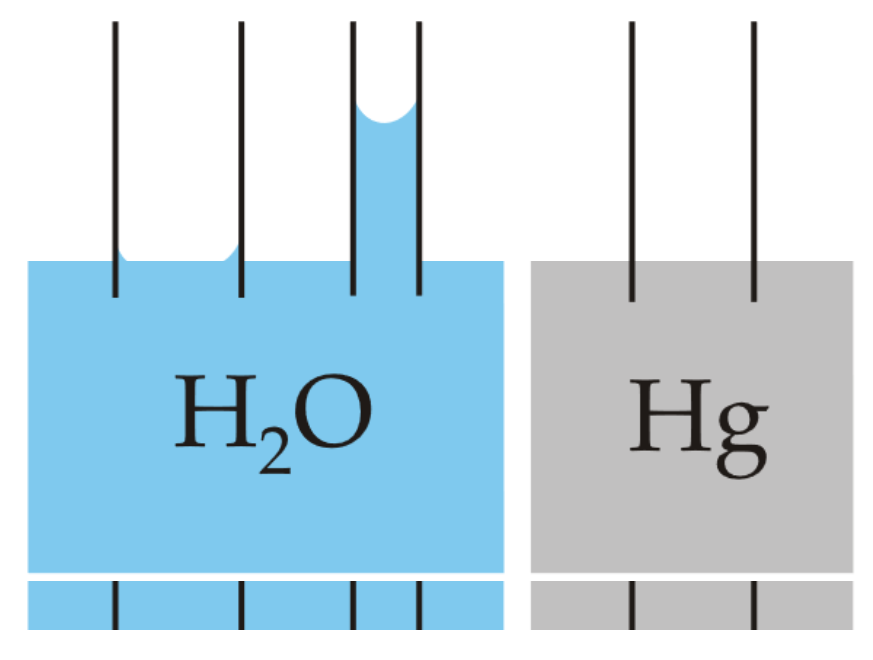
\includegraphics[width=0.4\textwidth]{capillary_tube.png}
\caption{竖直毛细管中的润湿（水）与不润湿（汞）（需插入原PPT第20次课第6页图片）}
\label{fig:capillary}
\end{figure}

\textbf{润湿}（如水在玻璃管中）：液面上升；\textbf{不润湿}（如水银在玻璃管中）：液面下降。

设液面为球冠，限制条件为液体体积守恒：
\begin{equation}
V = \pi h^2\left(R-\frac{h}{3}\right) = \text{const}.
\end{equation}

变分得
\begin{equation}
\mathrm{d}V=0\ \Rightarrow\ 2hR\,\mathrm{d}h+h^2\,\mathrm{d}R-h^2\,\mathrm{d}h=0
\ \Rightarrow\ h\,\mathrm{d}R=(h-2R)\,\mathrm{d}h.
\end{equation}

由热力学平衡（或力学平衡）：
\begin{equation}
\frac{\alpha_{sl}-\alpha_{sg}}{\alpha_{gl}}
= \frac{R\,\mathrm{d}h+h\,\mathrm{d}R}{h\,\mathrm{d}h-R\,\mathrm{d}h-h\,\mathrm{d}R}
= \frac{(h-R)\,\mathrm{d}h}{R\,\mathrm{d}h}
= -\frac{R-h}{R}
= -\cos\theta.
\end{equation}

于是得到与杨氏方程一致的结果：
\begin{equation}
\boxed{\cos\theta = \frac{\alpha_{sg}-\alpha_{sl}}{\alpha_{gl}} = \frac{R-h}{R}}
\end{equation}

\textbf{润湿现象的应用}：用钢笔写字、焊接金属（助焊剂）、浮游选矿等。

\subsubsection*{从热力学函数考虑}

总表面自由能
\begin{equation}
F = \alpha_{sl}A_{sl} + \alpha_{sg}A_{sg} + \alpha_{gl}A_{gl}.
\end{equation}

对于球冠形液滴（或液面），设固体表面为圆形，半径为 $R$，液面高度为 $h$，则
\begin{equation}
F = \alpha_{sg}A_{sg,\text{total}} + (\alpha_{sl}-\alpha_{sg})\pi[R^2-(R-h)^2] + \alpha_{gl}\cdot 2\pi Rh.
\end{equation}

平衡态时系统自由能最小，$\mathrm{d}F=0$。求极值：
\begin{equation}
(\alpha_{sl}-\alpha_{sg})(2h\,\mathrm{d}R+2R\,\mathrm{d}h-2h\,\mathrm{d}h) + \alpha_{gl}(2R\,\mathrm{d}h+2h\,\mathrm{d}R)=0.
\end{equation}

整理后同样可得杨氏方程。

\subsubsection*{粗糙表面}

对于粗糙表面，定义\textbf{粗糙度} $r$ 为真实表面与其投影的比值（$r>1$）。

\begin{figure}[htbp]
\centering
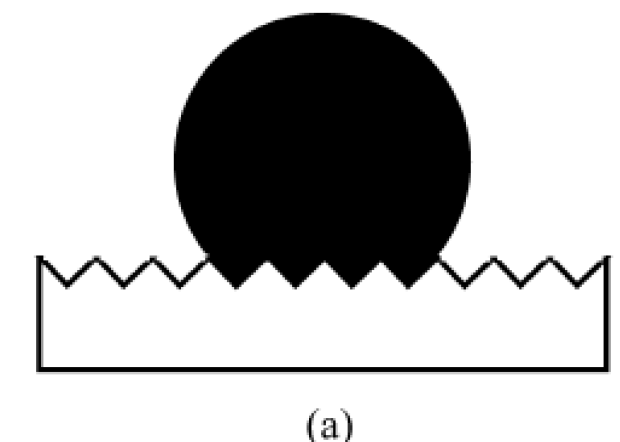
\includegraphics[width=0.35\textwidth]{rough_surface.png}
\caption{粗糙表面的接触角（需插入原PPT第20次课第6页图片）}
\label{fig:rough}
\end{figure}

总表面自由能
\begin{equation}
F = \alpha_{sg}A_{sg} + \alpha_{sl}A_{sl} + \alpha_{gl}A_{gl},
\end{equation}
其中各面积为真实面积。用投影面积表示：
\begin{equation}
F = \alpha_{sg}\cdot rA_{sg,\text{total}} - \alpha_{sg}\pi[R^2-(R-h)^2]r + \alpha_{sl}\pi[R^2-(R-h)^2]r + \alpha_{gl}\cdot 2\pi Rh.
\end{equation}

由平衡条件 $\mathrm{d}F=0$ 可得粗糙表面的接触角 $\theta_W$ 与光滑表面（杨氏）接触角 $\theta_Y$ 的关系：
\begin{equation}
\boxed{\cos\theta_W = r\frac{\alpha_{sg}-\alpha_{sl}}{\alpha_{gl}} = r\cos\theta_Y}
\end{equation}

\textbf{结论}：
\begin{itemize}
    \item 接触角小于 $90^\circ$（润湿），粗糙表面使接触角减小，润湿性增强；
    \item 接触角大于 $90^\circ$（不润湿），粗糙表面使接触角增大，不润湿性增强。
\end{itemize}

\subsubsection*{带气泡的粗糙表面}

对于粗糙表面，若液体未能完全填充粗糙表面的凹槽，则凹槽中可能截留气泡。此时系统包括固--气、固--液、液--气三个界面。

设总表面自由能为
\begin{equation}
F = \alpha_{sg}A_{sg} + \alpha_{sl}A_{sl} + \alpha_{gl}A_{gl}.
\end{equation}

用投影面积表示，设球冠形液滴在固体表面的投影半径为 $R$，液滴高度为 $h$，粗糙度为 $r$（真实表面与其投影的比值，$r>1$），$f$ 为投影面积中湿润部分（即固--液接触）的比值（$0<f\le 1$），则各界面面积为：
\begin{align}
A_{sg} &= A_{sg,\text{total}} - \pi\bigl[R^2-(R-h)^2\bigr]rf,\\
A_{sl} &= \pi\bigl[R^2-(R-h)^2\bigr]rf,\\
A_{gl} &= \pi\bigl[R^2-(R-h)^2\bigr](1-f) + 2\pi Rh.
\end{align}

由平衡条件 $\delta F=0$ 可得带气泡的粗糙表面的接触角 $\theta_{CD}$ 满足
\begin{equation}
\boxed{\cos\theta_{CD} = f - 1 + rf\cos\theta_Y}
\end{equation}
其中 $\theta_Y$ 为光滑表面的杨氏接触角。

\textbf{结论}：即使材料本身是浸润材料（$\theta_Y<\pi/2$），粗糙表面上被截留的气泡也会使表观接触角增大，甚至使其成为非浸润表面。

\begin{figure}[htbp]
\centering
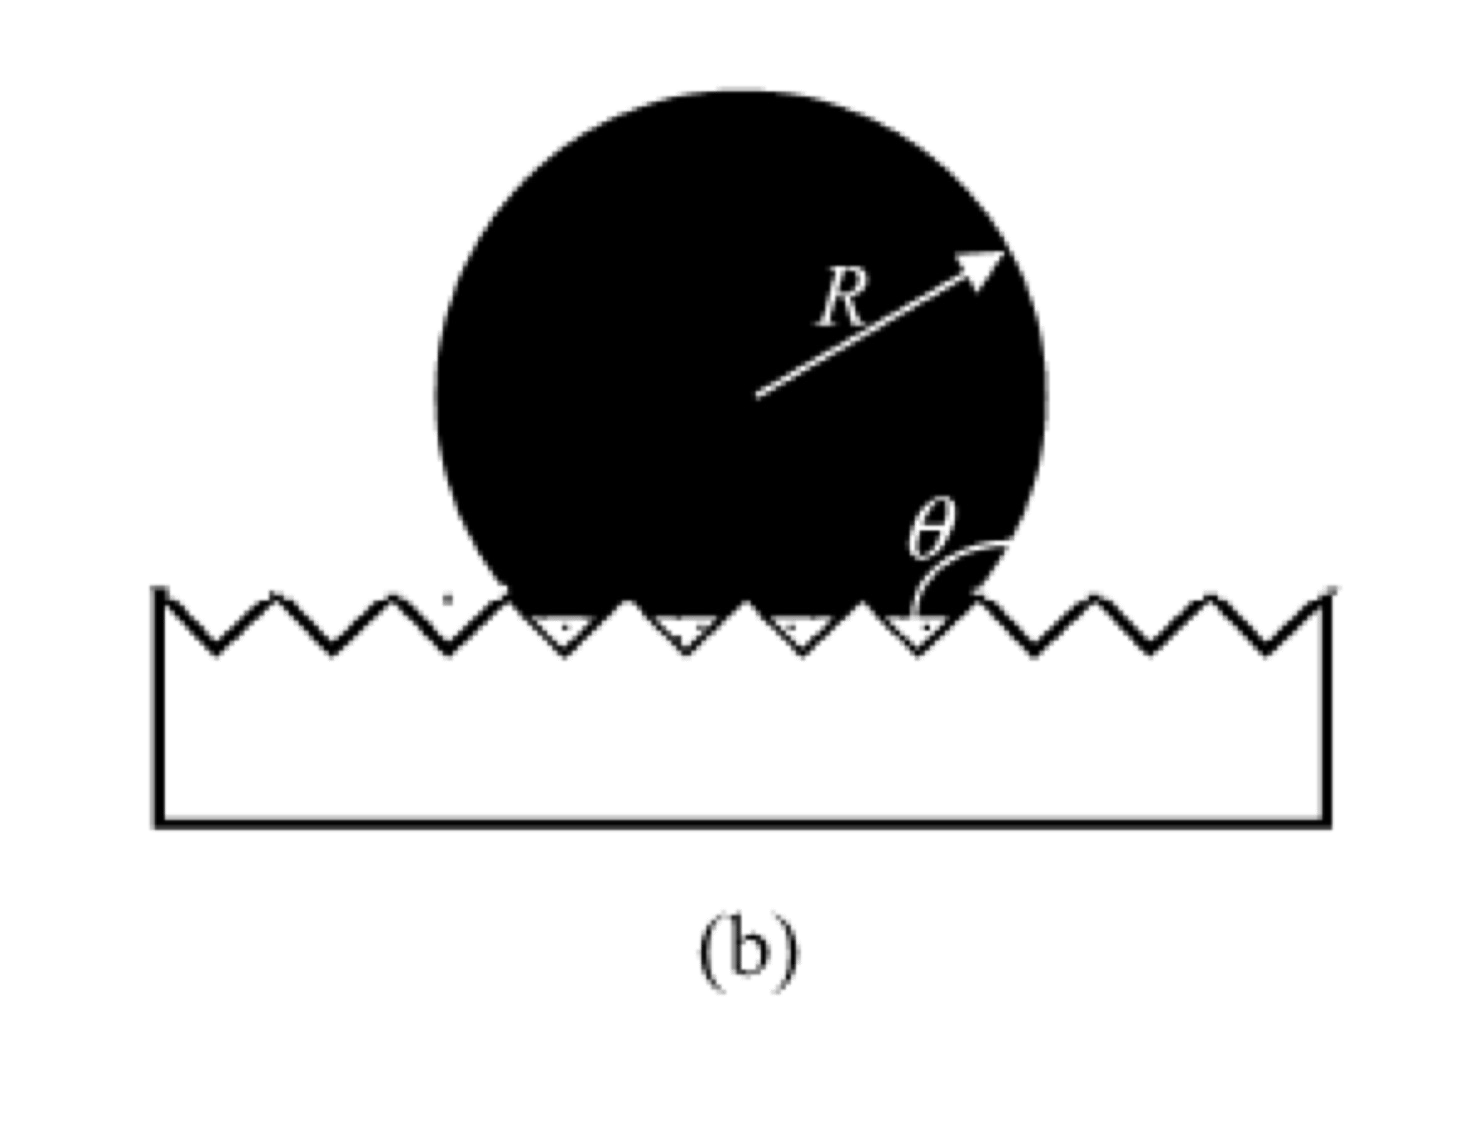
\includegraphics[width=0.35\textwidth]{rough_surface_bubble.png}
\caption{带气泡的粗糙表面接触角（需插入原PPT第20次课第3页图片）}
\label{fig:rough_bubble}
\end{figure}


\subsubsection*{超疏水与超亲水现象}

\textbf{超疏水}：通过表面微纳结构（如粗糙表面、微柱阵列）与低表面能材料相结合，可使表观接触角接近或大于 $150^\circ$，表现出极强的疏水性。例如水黾（water strider）能在水面行走，其腿部具有微纳多级刚毛结构，产生强烈的疏水力（江雷等，\textit{Nature} 2004, 432, 36）。

\textbf{人造荷叶}：通过模板法（如以荷叶为模板制备 PDMS 负模板，再翻模得到正模板）可人工制备具有微纳复合结构的超疏水表面（接触角 $>160^\circ$）。

\subsubsection*{毛细管液面高度}

\textbf{毛细现象}：将毛细管插入液体中，管内液面上升或下降的现象。其物理根源是液体的内聚力与附着力的竞争，即由弯曲液面内外的压强差决定。

柱形毛细管中液面呈球冠形。设毛细管半径为 $r$，液面曲率半径为 $R$，接触角为 $\theta$。取液面内外紧靠液面的两点 A（内侧）、D（外侧），以及平液面附近内外两点 C、O，如图。

\begin{figure}[htbp]
\centering
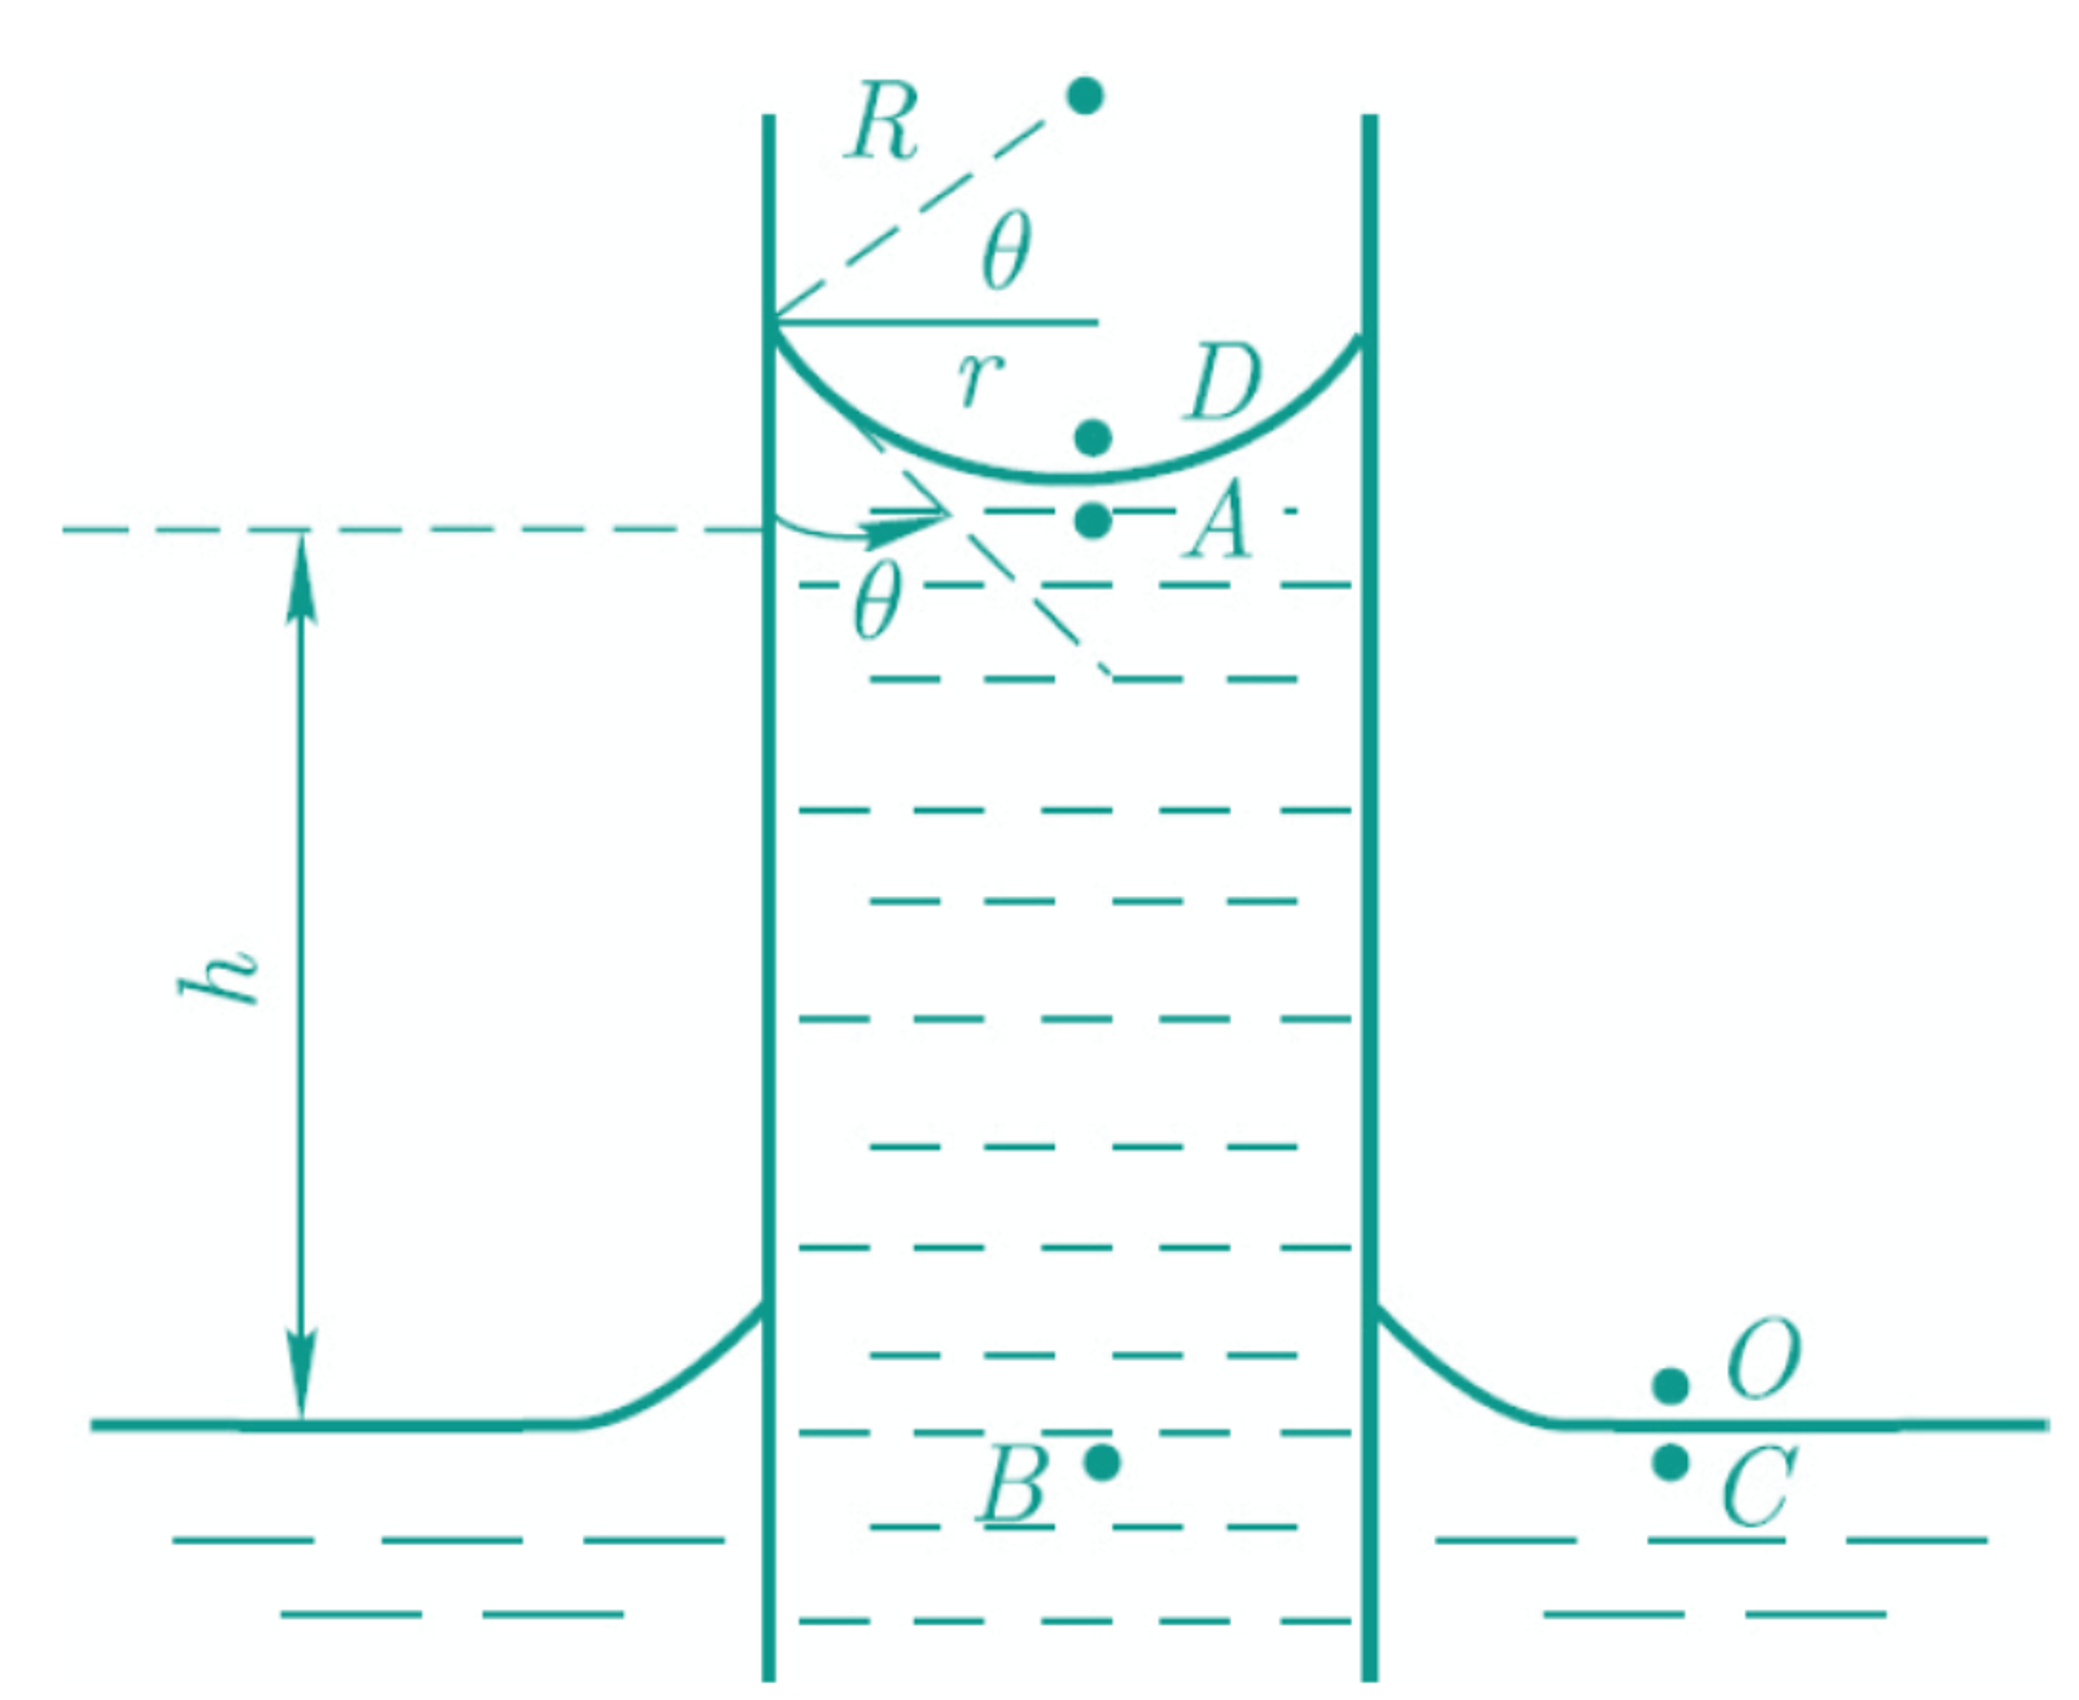
\includegraphics[width=0.4\textwidth]{capillary_height.png}
\caption{柱形毛细管中液面高度示意图（需插入原PPT第20次课第8--9页图片）}
\label{fig:capillary_height}
\end{figure}

由拉普拉斯公式，对球冠形凹液面（曲率中心在液面上方气相中，$R>0$）：
\begin{equation}
p_A - p_D = \frac{2\alpha}{R},\qquad p_A = p_D - \frac{2\alpha}{R} = p_0 - \frac{2\alpha}{R}.
\end{equation}

平液面处 $p_C=p_O=p_0$。显然 $p_A<p_C$，故液体进入毛细管，液面上升。设平衡时管内液面下方与 C 同高处为 B 点，液面上升高度为 $h$，则
\begin{equation}
p_B = p_A + \rho gh = p_0 - \frac{2\alpha}{R} + \rho gh.
\end{equation}

因 $p_B=p_C=p_0$，于是
\begin{equation}
p_0 - \frac{2\alpha}{R} + \rho gh = p_0
\quad\Rightarrow\quad
\boxed{h = \frac{2\alpha}{\rho gR} = \frac{2\alpha\cos\theta}{\rho gr}}.
\end{equation}

其中几何关系 $R = r/\cos\theta$（由球冠几何，接触角 $\theta$ 满足 $r=R\cos\theta$）。

\textbf{讨论}：
\begin{itemize}
\item $0\le\theta<\pi/2$（润湿）：$h>0$，管内液面上升；
\item $\pi/2<\theta\le\pi$（不润湿）：$h<<0$，管内液面下降。
\end{itemize}


\subsubsection*{两平板间液面的高度}

\paragraph{平行板}

两平行竖直板之间液面呈柱面（柱形液面）。设两板间距为 $d$，由柱面的拉普拉斯公式 $\Delta p = \alpha/R$，其中曲率半径 $R = d/(2\cos\theta)$，可得液面上升高度
\begin{equation}
\boxed{h = \frac{\alpha\cos\theta}{\rho g\,\dfrac{d}{2}} = \frac{2\alpha\cos\theta}{\rho gd}}.
\end{equation}

\textbf{讨论}：
\begin{itemize}
\item $0\le\theta<\pi/2$：$h>0$，内部液面上升；
\item $\pi/2<\theta\le\pi$：$h<<0$，内部液面下降。
\end{itemize}

\paragraph{相交板}

两平板相交成很小夹角 $\varphi$，建立坐标系使交线水平，$x$ 轴沿交线垂直方向。$x$ 处两板间距 $d=x\varphi$，代入平行板公式得
\begin{equation}
h(x) = \frac{2\alpha\cos\theta}{\rho g x\varphi}.
\end{equation}
液面呈双曲面形（双曲型液面）。

\begin{figure}[htbp]
\centering
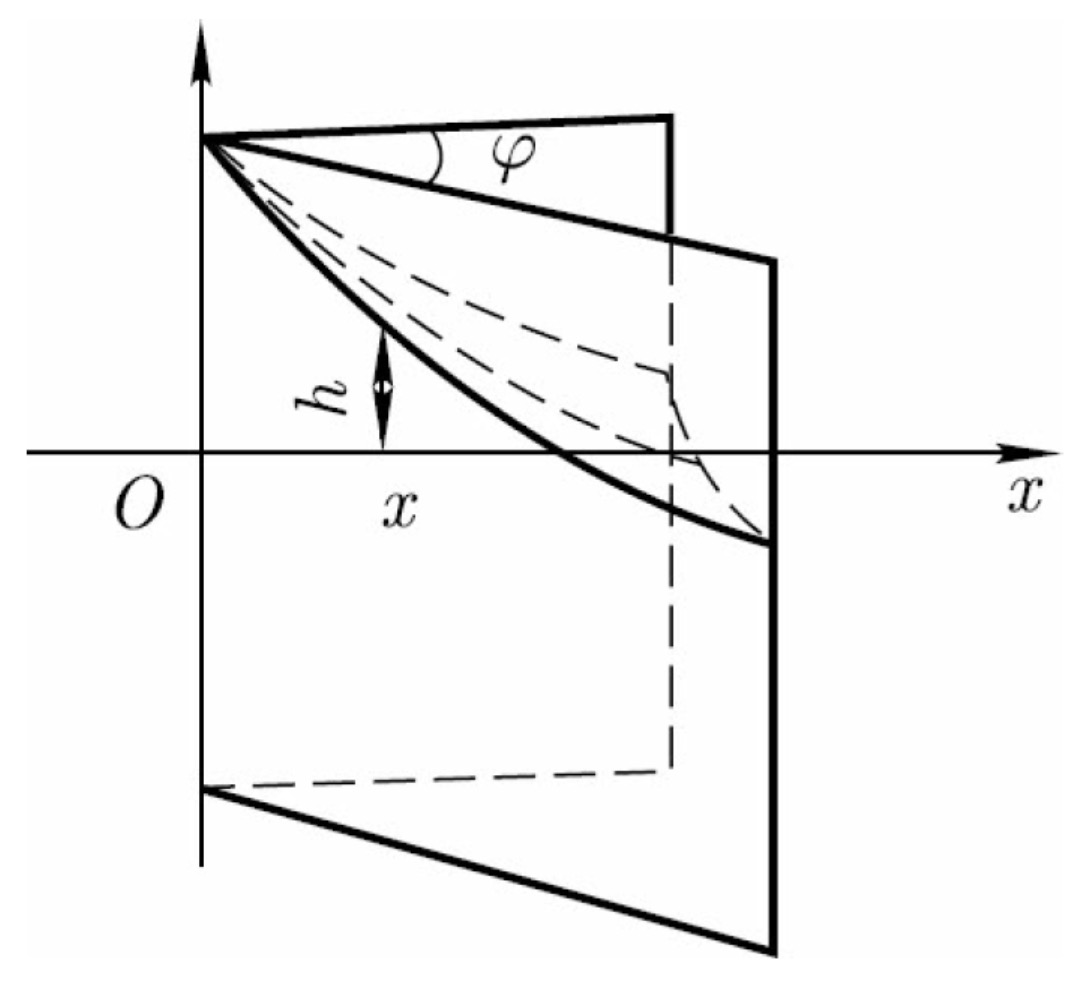
\includegraphics[width=0.4\textwidth]{parallel_plates_capillary.png}
\caption{两平行板与相交板间的毛细液面（需插入原PPT第20次课第10页图片）}
\label{fig:parallel_plates}
\end{figure}


\subsubsection*{例题：U型管水面高度差}

\textbf{题目}：如图，一U型玻璃管两管直径分别为 $d_1=1\,\mathrm{mm}$，$d_2=3\,\mathrm{mm}$，设水完全润湿玻璃（接触角 $\theta=0$），大气压强为 $p_0$，求两管中水面高度差。

\begin{figure}[htbp]
\centering
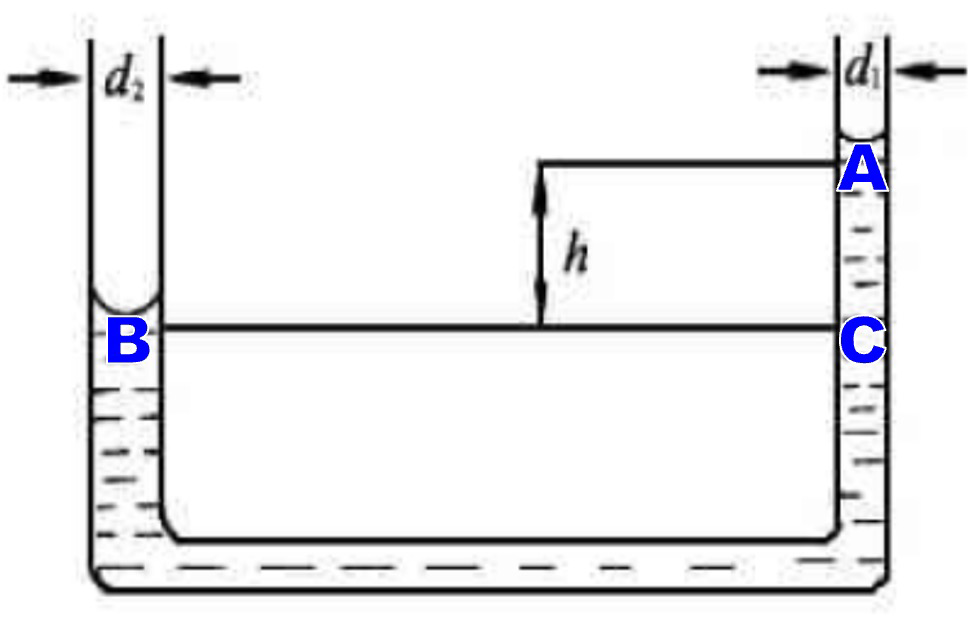
\includegraphics[width=0.4\textwidth]{u_tube_capillary.png}
\caption{U型毛细管水面高度差（需插入原PPT第20次课第11--12页图片）}
\label{fig:u_tube}
\end{figure}

\textbf{解}：水完全润湿玻璃，液面为凹球冠，接触角 $\theta=0$，曲率半径 $R_i=d_i/2$。

对细管（直径 $d_1$）液面内侧紧靠液面的 A 点：
\begin{equation}
p_A = p_0 - \frac{2\alpha}{R_1} = p_0 - \frac{4\alpha}{d_1}.
\end{equation}

对粗管（直径 $d_2$）液面内侧紧靠液面的 B 点：
\begin{equation}
p_B = p_0 - \frac{4\alpha}{d_2}.
\end{equation}

设细管中与 B 同高的点为 C，则 $p_B=p_C$，且 $p_C = p_A + \rho gh$。于是
\begin{equation}
p_0 - \frac{4\alpha}{d_2} = p_0 - \frac{4\alpha}{d_1} + \rho gh,
\end{equation}
解得
\begin{equation}
\boxed{h = \frac{4\alpha}{\rho g}\left(\frac{1}{d_1}-\frac{1}{d_2}\right)}.
\end{equation}

代入水的表面张力系数 $\alpha\approx 73\times10^{-3}\,\mathrm{N/m}$，$\rho=10^3\,\mathrm{kg/m^3}$，$g=9.8\,\mathrm{m/s^2}$，$d_1=1\,\mathrm{mm}$，$d_2=3\,\mathrm{mm}$：
\begin{equation}
h = \frac{4\times73\times10^{-3}}{10^3\times9.8}\left(\frac{1}{10^{-3}}-\frac{1}{3\times10^{-3}}\right)\,\mathrm{m}
\approx 2\times10^{-2}\,\mathrm{m} = 0.02\,\mathrm{m}.
\end{equation}

\textbf{应用}：植物中营养和水分的传输；农业生产中翻耕土地以破坏毛细管，减少水分蒸发。

\newpage
% ============================================
\section{第七章：单元系统的复相平衡与相变}
% ============================================

% --------------------------------------------
\subsection{化学势}
% --------------------------------------------

\subsubsection*{化学势的定义}

\textbf{化学势} $\mu$：若向系统中加入一个粒子而不改变系统的体积和熵，则系统内能的改变量即为化学势
\begin{equation}
\mu = \left(\frac{\partial U}{\partial N}\right)_{S,V}.
\end{equation}

由于 $S$ 和 $V$ 在实验中很难直接约束，更常用的定义是从其他热力学势导出：

由热力学基本方程的推广（开放系统）：
\begin{align}
\mathrm{d}U &= T\,\mathrm{d}S - p\,\mathrm{d}V + \mu\,\mathrm{d}N, \\
\mathrm{d}F &= -S\,\mathrm{d}T - p\,\mathrm{d}V + \mu\,\mathrm{d}N, \\
\mathrm{d}G &= -S\,\mathrm{d}T + V\,\mathrm{d}p + \mu\,\mathrm{d}N,
\end{align}
可得
\begin{equation}
\mu = \left(\frac{\partial U}{\partial N}\right)_{S,V}
= \left(\frac{\partial F}{\partial N}\right)_{V,T}
= \left(\frac{\partial G}{\partial N}\right)_{p,T}.
\end{equation}

\textbf{开放系统的热力学基本方程}（多组分系统）：
\begin{align}
\mathrm{d}U &= T\,\mathrm{d}S - p\,\mathrm{d}V + \sum_i\mu_i\,\mathrm{d}N_i, \\
\mathrm{d}H &= T\,\mathrm{d}S + V\,\mathrm{d}p + \sum_i\mu_i\,\mathrm{d}N_i, \\
\mathrm{d}F &= -S\,\mathrm{d}T - p\,\mathrm{d}V + \sum_i\mu_i\,\mathrm{d}N_i, \\
\mathrm{d}G &= -S\,\mathrm{d}T + V\,\mathrm{d}p + \sum_i\mu_i\,\mathrm{d}N_i.
\end{align}


\subsubsection*{化学势的新解释}

若系统的大小改变一个因子 $\lambda$，则各\textbf{广延量}相应改变：
\begin{equation}
U\to\lambda U,\quad S\to\lambda S,\quad V\to\lambda V,\quad N\to\lambda N.
\end{equation}

由熵的广延性：
\begin{equation}
\lambda S(U,V,N) = S(\lambda U,\lambda V,\lambda N).
\end{equation}

两边对 $\lambda$ 求导，利用链式法则：
\begin{equation}
S = \frac{\partial S}{\partial(\lambda U)}\frac{\partial(\lambda U)}{\partial\lambda}
+ \frac{\partial S}{\partial(\lambda V)}\frac{\partial(\lambda V)}{\partial\lambda}
+ \frac{\partial S}{\partial(\lambda N)}\frac{\partial(\lambda N)}{\partial\lambda}.
\end{equation}

令 $\lambda=1$，并注意
\begin{equation}
\frac{\partial S}{\partial U} = \frac{1}{T},\quad
\frac{\partial S}{\partial V} = \frac{p}{T},\quad
\frac{\partial S}{\partial N} = -\frac{\mu}{T},
\end{equation}
得
\begin{equation}
S = \frac{U}{T} + \frac{pV}{T} - \frac{\mu N}{T}.
\end{equation}

整理得
\begin{equation}
U - TS + pV = \mu N.
\end{equation}

由吉布斯函数定义 $G = U - TS + pV$，故
\begin{equation}
\boxed{G = \mu N,\qquad \mu = \frac{G}{N}}
\end{equation}
即\textbf{化学势等于单粒子的吉布斯函数}。


% --------------------------------------------
\subsection{相、相变及相平衡的概念}
% --------------------------------------------

\subsubsection*{相的概念与相稳定条件}

\textbf{相}：在没有外界影响下，被一定边界包围的，具有确定并且均匀的物理和化学性质的一个系统（或系统的一部分）所处的状态称为物质的一个相。

\textbf{相稳定条件}：系统处于平衡态时，对各种可能的涨落（体积涨落、熵涨落、粒子数涨落）必须稳定。下面分别讨论。

\paragraph{体积涨落}

设系统由两个全同子系统组成，每一子系统的自由焓为 $G(V,S,N)$，则总自由焓 $G_t=2G(V,S,N)$。假设在等温、等压条件下发生一个体积涨落（总体积不变），此时总自由焓为
\begin{equation}
G(V+\Delta V,S) + G(V-\Delta V,S).
\end{equation}

系统在热力学平衡态时自由焓极小，故
\begin{equation}
G(V+\Delta V,S) + G(V-\Delta V,S) \ge 2G(V,S).
\end{equation}

设此过程为等熵过程，$G=H-TS=U+pV-TS$，对 $G(V\pm\Delta V,S)$ 作泰勒展开：
\begin{equation}
G(V\pm\Delta V,S) \approx G(V,S) \pm \left(\frac{\partial U}{\partial V}\right)_S\Delta V
+ \frac{1}{2}\left(\frac{\partial^2 U}{\partial V^2}\right)_S(\Delta V)^2 \pm p\Delta V.
\end{equation}

代入不等式，利用 $\displaystyle\left(\frac{\partial U}{\partial V}\right)_S=-p$，得
\begin{equation}
\left(\frac{\partial^2 U}{\partial V^2}\right)_S(\Delta V)^2 \ge 0
\quad\Rightarrow\quad
\left(\frac{\partial^2 U}{\partial V^2}\right)_S \ge 0.
\end{equation}

考虑 $\displaystyle\left(\frac{\partial U}{\partial V}\right)_S=-p$，则
\begin{equation}
-\left(\frac{\partial p}{\partial V}\right)_S \ge 0.
\end{equation}

定义\textbf{绝热压缩系数}
\begin{equation}
\kappa_S = -\frac{1}{V}\left(\frac{\partial V}{\partial p}\right)_S,
\end{equation}
则平衡态稳定条件化为
\begin{equation}
\boxed{\kappa_S \ge 0}
\end{equation}

\textbf{结论}：体积涨落下能自动回到平衡态的必要条件为\textbf{绝热压缩系数大于零}。

\paragraph{熵涨落}

假设两系统在等容条件下有一个熵涨落（总熵不变），总自由焓为 $G(V,S+\Delta S)+G(V,S-\Delta S)$。平衡时自由焓极小：
\begin{equation}
G(V,S+\Delta S) + G(V,S-\Delta S) - 2G(V,S) \ge 0.
\end{equation}

类似展开，利用 $\displaystyle\left(\frac{\partial U}{\partial S}\right)_V=T$，得平衡态稳定条件
\begin{equation}
\left(\frac{\partial^2 U}{\partial S^2}\right)_V \ge 0.
\end{equation}

由于
\begin{equation}
\left(\frac{\partial^2 U}{\partial S^2}\right)_V = \left(\frac{\partial T}{\partial S}\right)_V
= \frac{T}{C_V},
\end{equation}
故
\begin{equation}
\boxed{C_V > 0}
\end{equation}

\paragraph{粒子数涨落}

考虑粒子数涨落，可得
\begin{equation}
\left(\frac{\partial^2 G}{\partial N^2}\right)_{V,S} \ge 0
\quad\Rightarrow\quad
\left(\frac{\partial\mu}{\partial N}\right)_{V,S} > 0.
\end{equation}

\paragraph{一般平衡态稳定条件}

综合以上三种涨落，一般情况下的平衡态稳定条件为
\begin{equation}
\boxed{\left(\frac{\partial\mu}{\partial N}\right)_{V,S} > 0,\quad C_V > 0,\quad \kappa_S > 0}
\end{equation}

对理想气体，由等温过程方程 $pV=\text{const}$ 得
\begin{equation}
\left(\frac{\partial p}{\partial V}\right)_T = -\frac{p}{V}.
\end{equation}

由绝热过程方程 $pV^\gamma=\text{const}$ 得
\begin{equation}
\left(\frac{\partial p}{\partial V}\right)_S = -\gamma\frac{p}{V}.
\end{equation}

于是
\begin{equation}
\frac{(\partial p/\partial V)_S}{(\partial p/\partial V)_T}
= \frac{(\partial V/\partial p)_T}{(\partial V/\partial p)_S}
= \frac{-V\kappa_T}{-V\kappa_S}
= \frac{\kappa_T}{\kappa_S} = \gamma.
\end{equation}

\textbf{结论}：对于理想气体，等温压缩系数正比于等熵压缩系数。一般情况，$\kappa_S$ 与 $\kappa_T$ 符号相同，故平衡态稳定条件也可写为
\begin{equation}
\boxed{\left(\frac{\partial\mu}{\partial N}\right)_{V,S} > 0,\quad C_V > 0,\quad \kappa_T > 0}
\end{equation}


\subsubsection*{相变及其分类}

\textbf{相变}：物质在压强、温度等外界条件不变的情况下，从一个相转变为另一个相的现象。相变过程是物质结构发生突然变化的过程，常伴随某种物质性质的突然变化。

\textbf{按物理性质变化分类}：
\begin{itemize}
\item \textbf{一级相变}：相变发生时，两相之间有潜热和体积等跃变。如：液--气相变。
\item \textbf{二级相变}：相变发生时，两相之间无潜热和体积等跃变，但有热容跃变。如：超导相变、液氦相变。
\end{itemize}

\textbf{用数学方法分类}（以吉布斯函数 $G$ 为判据）：
\begin{itemize}
\item \textbf{一级相变}：热力学函数 $G$ 连续，但其状态参量的一阶导数不连续。
\item \textbf{二级相变}：热力学函数 $G$ 及其关于状态参量的一阶导数都连续，但其关于状态参量的二阶导数不连续。
\end{itemize}

\textbf{对 $p$--$V$--$T$ 系统}：设相变在等温等压条件下进行，$\mathrm{d}G=V\,\mathrm{d}p-S\,\mathrm{d}T$，则
\begin{equation}
V = \left(\frac{\partial G}{\partial p}\right)_T,\qquad
S = -\left(\frac{\partial G}{\partial T}\right)_p.
\end{equation}

相变时：
\begin{itemize}
\item \textbf{体积跃变}
\begin{equation}
\Delta V = V_{II}-V_I = \left[\left(\frac{\partial G}{\partial p}\right)_T\right]_{II} - \left[\left(\frac{\partial G}{\partial p}\right)_T\right]_I
\end{equation}
对应 $(\partial G/\partial p)_T$ 不连续，为\textbf{一级相变}（能量的转化）。

\item \textbf{相变潜热}
\begin{equation}
\Lambda = H_{II}-H_I = T\Delta S = T\left\{\left[\left(\frac{\partial G}{\partial T}\right)_p\right]_I - \left[\left(\frac{\partial G}{\partial T}\right)_p\right]_{II}\right\}
\end{equation}
对应 $(\partial G/\partial T)_p$ 不连续，亦为\textbf{一级相变}。

\item \textbf{热容跃变}
\begin{equation}
\left(\frac{\partial^2 G}{\partial T^2}\right)_p = -\left(\frac{\partial S}{\partial T}\right)_p = -\frac{C_p}{T}
\end{equation}
若 $(\partial^2 G/\partial T^2)_p$ 不连续，则导致\textbf{热容跃变}，对应\textbf{二级相变}（对称性的变化）。
\end{itemize}


\subsubsection*{相平衡及相图}

\textbf{相平衡}：是一个动态平衡。

\textbf{相图}（phase diagram）：把一物质系统的相、相变及相平衡以其状态参量为变量所作的图示。常见曲线包括：
\begin{itemize}
\item \textbf{汽化曲线}：液--气两相平衡曲线；
\item \textbf{熔解曲线}：固--液两相平衡曲线；
\item \textbf{升华曲线}：固--气两相平衡曲线。
\end{itemize}

\begin{figure}[htbp]
\centering
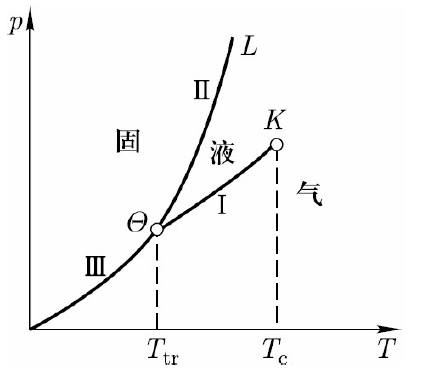
\includegraphics[width=0.4\textwidth]{phase_diagram.png}
\caption{典型单元系相图（$p$-$T$ 图）：固、液、气三相及三相点 $\Theta$、临界点 $K$（需插入原PPT第25页图片）}
\label{fig:phase_diagram}
\end{figure}

\textbf{临界温度} $T_c$：在温度低于临界温度时，系统可以发生有液--气共存状态的一级相变（有摩尔体积突变）；在临界温度 $T_c$ 之上，系统不再有液--气共存状态，即不再能发生一级相变。图中 $T_{\mathrm{tr}}$ 为\textbf{三相点温度}。

\begin{center}
\begin{tabular}{c|c|c}
\hline
曲线 & 名称 & 相平衡 \\
\hline
I & 汽化曲线 & 液 $\rightleftharpoons$ 气 \\
II & 熔解曲线 & 固 $\rightleftharpoons$ 液 \\
III & 升华曲线 & 固 $\rightleftharpoons$ 气 \\
\hline
\end{tabular}
\end{center}

% --------------------------------------------
\subsection{单元系的复相平衡}
% --------------------------------------------

\subsubsection*{复相平衡条件}

假设一个单元系的两相（$\alpha$相和$\beta$相）已达到相平衡，并且该单元系的这两个相与其它系统隔绝。对于一级相变，$\alpha$相和$\beta$相的总内能$U_\alpha+U_\beta$，总体积$V_\alpha+V_\beta$，总粒子数$N_\alpha+N_\beta$是守恒的。

设想在两相之间有一个微小的变动，则孤立系的平衡要求
\begin{equation}
\mathrm{d}U_\alpha+\mathrm{d}U_\beta=0,\qquad
\mathrm{d}V_\alpha+\mathrm{d}V_\beta=0,\qquad
\mathrm{d}N_\alpha+\mathrm{d}N_\beta=0.
\end{equation}

由开放系统的热力学基本方程
\begin{equation}
\mathrm{d}U = T\,\mathrm{d}S - p\,\mathrm{d}V + \mu\,\mathrm{d}N,
\end{equation}
可得各相的熵变：
\begin{equation}
\mathrm{d}S_\alpha = \frac{\mathrm{d}U_\alpha+p_\alpha\,\mathrm{d}V_\alpha-\mu_\alpha\,\mathrm{d}N_\alpha}{T_\alpha},
\qquad
\mathrm{d}S_\beta = \frac{\mathrm{d}U_\beta+p_\beta\,\mathrm{d}V_\beta-\mu_\beta\,\mathrm{d}N_\beta}{T_\beta}.
\end{equation}

系统的总熵变
\begin{equation}
\mathrm{d}S = \mathrm{d}S_\alpha+\mathrm{d}S_\beta
= \frac{\mathrm{d}U_\alpha+p_\alpha\,\mathrm{d}V_\alpha-\mu_\alpha\,\mathrm{d}N_\alpha}{T_\alpha}
+ \frac{\mathrm{d}U_\beta+p_\beta\,\mathrm{d}V_\beta-\mu_\beta\,\mathrm{d}N_\beta}{T_\beta}.
\end{equation}

利用守恒条件$\mathrm{d}U_\beta=-\mathrm{d}U_\alpha$等代入，整理得
\begin{equation}
\mathrm{d}S
= \mathrm{d}U_\alpha\!\left(\frac{1}{T_\alpha}-\frac{1}{T_\beta}\right)
+ \mathrm{d}V_\alpha\!\left(\frac{p_\alpha}{T_\alpha}-\frac{p_\beta}{T_\beta}\right)
- \mathrm{d}N_\alpha\!\left(\frac{\mu_\alpha}{T_\alpha}-\frac{\mu_\beta}{T_\beta}\right).
\end{equation}

由于整个系统达到平衡时$\mathrm{d}S=0$，且$\mathrm{d}U_\alpha,\mathrm{d}V_\alpha,\mathrm{d}N_\alpha$相互独立，故两相平衡条件为
\begin{equation}
\boxed{T_\alpha=T_\beta,\qquad p_\alpha=p_\beta,\qquad \mu_\alpha=\mu_\beta}
\end{equation}
分别称为\textbf{热学平衡条件}、\textbf{力学平衡条件}和\textbf{化学平衡条件}。

\subsubsection*{化学势与相变方向}

处于平衡态、具有$n$个相的系统，每个相都满足热力学基本方程
\begin{equation}
\mathrm{d}G_i = -S_i\,\mathrm{d}T + V_i\,\mathrm{d}p + \mu_i\,\mathrm{d}N_i,\qquad i=1,2,\dots,n.
\end{equation}

整个系统也满足热力学基本方程：
\begin{equation}
\mathrm{d}G = -S\,\mathrm{d}T + V\,\mathrm{d}p + \sum_{i=1}^{n}\mu_i\,\mathrm{d}N_i,
\end{equation}
其中$S=\sum_i S_i,\ V=\sum_i V_i$。

由自由焓判据知，对于$n=2$的等温、等压系统：
\begin{equation}
\mathrm{d}G = \mathrm{d}G_1+\mathrm{d}G_2 = \mu_1\,\mathrm{d}N_1+\mu_2\,\mathrm{d}N_2
= (\mu_1-\mu_2)\,\mathrm{d}N_1\le 0.
\end{equation}

因此：
\begin{itemize}
\item 若$\mu_1>\mu_2$，则$\mathrm{d}N_1<<0,\ \mathrm{d}N_2>0$；``1''相减少，``2''相增加；
\item 若$\mu_1<\mu_2$，则$\mathrm{d}N_1>0,\ \mathrm{d}N_2<<0$；``2''相减少，``1''相增加。
\end{itemize}

\textbf{自发过程是物质从化学势高的相向化学势低的相转移。}


% --------------------------------------------
\subsection{单元系复相平衡的性质}
% --------------------------------------------

\subsubsection*{克拉珀龙方程}

由相平衡条件知，在平衡曲线上有
\begin{equation}
\mu_\alpha(T,p)=\mu_\beta(T,p),
\end{equation}
且对其微分后仍有
\begin{equation}
\mu_\alpha(T+\mathrm{d}T,p+\mathrm{d}p)=\mu_\beta(T+\mathrm{d}T,p+\mathrm{d}p).
\end{equation}

两式相减得
\begin{equation}
\mathrm{d}\mu_\alpha
= \left(\frac{\partial\mu_\alpha}{\partial T}\right)_p\mathrm{d}T + \left(\frac{\partial\mu_\alpha}{\partial p}\right)_T\mathrm{d}p
= \mathrm{d}\mu_\beta
= \left(\frac{\partial\mu_\beta}{\partial T}\right)_p\mathrm{d}T + \left(\frac{\partial\mu_\beta}{\partial p}\right)_T\mathrm{d}p.
\end{equation}

由化学势的定义$\displaystyle\mu=\left(\frac{\partial G}{\partial N}\right)_{T,p}=\frac{G}{N}=\frac{G_m}{N_A}$及热力学基本方程$\mathrm{d}G=-S\,\mathrm{d}T+V\,\mathrm{d}p$，得
\begin{equation}
\left(\frac{\partial\mu_\alpha}{\partial T}\right)_p = -\frac{1}{N_A}S_{\alpha,m},\qquad
\left(\frac{\partial\mu_\alpha}{\partial p}\right)_T = \frac{1}{N_A}V_{\alpha,m},
\end{equation}
其中$S_m,V_m$分别是系统的摩尔熵、摩尔体积。

代入整理得
\begin{equation}
-S_{\alpha,m}\,\mathrm{d}T + V_{\alpha,m}\,\mathrm{d}p
= -S_{\beta,m}\,\mathrm{d}T + V_{\beta,m}\,\mathrm{d}p,
\end{equation}
即
\begin{equation}
\frac{\mathrm{d}p}{\mathrm{d}T}
= \frac{S_{\beta,m}-S_{\alpha,m}}{V_{\beta,m}-V_{\alpha,m}}.
\end{equation}

一级相变中，摩尔相变潜热$\Lambda_m=T(S_{\beta,m}-S_{\alpha,m})$，于是得到\textbf{克拉珀龙方程}（Clapeyron equation）：
\begin{equation}
\boxed{\frac{\mathrm{d}p}{\mathrm{d}T} = \frac{\Lambda_m}{T\,(V_{\beta,m}-V_{\alpha,m})}}
\end{equation}
亦称\textbf{克拉珀龙--克劳修斯方程}。

\begin{figure}[htbp]
\centering
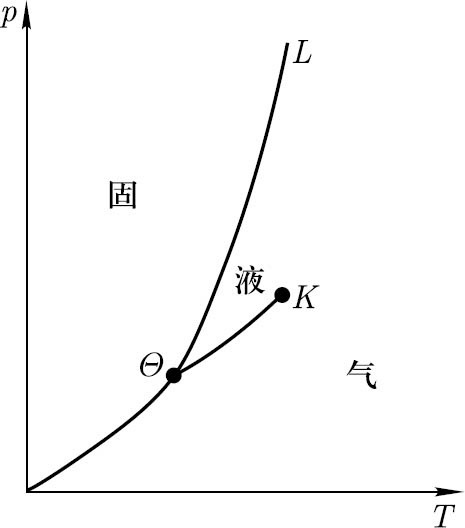
\includegraphics[width=0.35\textwidth]{clapeyron_pt_diagram.png}
\caption{单元系$p$-$T$相图与相平衡曲线（示意，需插入原PPT第22次课第5页图片）}
\label{fig:clapeyron_pt}
\end{figure}


\subsubsection*{例题：冰的熔点与滑冰}

\textbf{题目}：冰在$1\,\mathrm{atm}$下熔点为$273.15\,\mathrm{K}$，冰和水的摩尔体积分别为$V_{\text{冰}}^{\mathrm{mol}}=1.965\times10^{-5}\,\mathrm{m^3/mol}$和$V_{\text{水}}^{\mathrm{mol}}=1.8019\times10^{-5}\,\mathrm{m^3/mol}$，熔解热为$\Lambda^{\mathrm{mol}}=1.436\,\mathrm{kcal/mol}$，求熔点随压强的变化率。

\textbf{解}：由克拉珀龙方程
\begin{equation}
\frac{\mathrm{d}p}{\mathrm{d}T}
= \frac{\Lambda^{\mathrm{mol}}}{T\bigl(V_{\text{水}}^{\mathrm{mol}}-V_{\text{冰}}^{\mathrm{mol}}\bigr)}
= \frac{1.436\times10^3\times4.184}{273.15\times(1.8019-1.965)\times10^{-5}}
\approx -1.348\times10^7\,\mathrm{N/(m^2\cdot K)}
= -1.330\times10^2\,\mathrm{atm/K}.
\end{equation}

故熔点随压强的变化率
\begin{equation}
\frac{\mathrm{d}T}{\mathrm{d}p} = -7.519\times10^{-3}\,\mathrm{K/atm}.
\end{equation}

\textbf{滑冰问题}：设冰鞋与冰面接触面积为$0.3\,\mathrm{cm}\times40\,\mathrm{cm}=12\,\mathrm{cm^2}=1.2\times10^{-3}\,\mathrm{m^2}$，人重$100\,\mathrm{kg}$，则附加压强
\begin{equation}
\mathrm{d}p = \frac{100\times9.8}{1.2\times10^{-3}}
= 8.16\times10^5\,\mathrm{N/m^2}\approx 8.1\,\mathrm{atm}.
\end{equation}

对应的熔点变化
\begin{equation}
\mathrm{d}T \approx -0.06\,\mathrm{K}.
\end{equation}

\textbf{讨论}：冰面为什么是滑的？历史上曾有``压力融解说''、``摩擦融解说''、``表面融化说''等不同解释，实际可能是多种机制共同作用的结果。


\subsubsection*{例题：水的沸点与饱和蒸汽压}

\textbf{题目}：水在$1\,\mathrm{atm}$下的沸点为$373.15\,\mathrm{K}$，此时水蒸气与水的摩尔体积分别为$V_g^{\mathrm{mol}}=3.0139\times10^{-2}\,\mathrm{m^3/mol}$与$V_l^{\mathrm{mol}}=1.8798\times10^{-5}\,\mathrm{m^3/mol}$，摩尔汽化热为$\Lambda^{\mathrm{mol}}=9.7126\,\mathrm{kcal/mol}$，求饱和蒸汽压随温度的变化率和沸点与压强的关系。

\textbf{解}：饱和蒸汽压随温度的变化率由克拉珀龙方程得
\begin{equation}
\frac{\mathrm{d}p}{\mathrm{d}T}
= \frac{\Lambda^{\mathrm{mol}}}{T\bigl(V_g^{\mathrm{mol}}-V_l^{\mathrm{mol}}\bigr)}
= \frac{9.7126\times10^3\times4.184}{373.15\times(3.0139\times10^{-2}-1.8798\times10^{-5})}
\approx 3.6157\times10^3\,\mathrm{N/(m^2\cdot K)}
= 3.568\times10^{-2}\,\mathrm{atm/K}.
\end{equation}

沸点与压强的关系：
\begin{equation}
\frac{\mathrm{d}T}{\mathrm{d}p} \approx 28.027\,\mathrm{K/atm}.
\end{equation}


\subsubsection*{例题：海拔对沸点的影响}

\textbf{题目}：已知水在$100^\circ\mathrm{C}$时的汽化热为$\Lambda=2.26\times10^6\,\mathrm{J/kg}$，设大气温度为$T_0=300\,\mathrm{K}$，试问从海平面每上升$1$千米，水的沸点变化多少？

\textbf{解}：大气压强随高度的变化满足
\begin{equation}
\frac{\mathrm{d}p}{\mathrm{d}z} = -\rho g.
\end{equation}

由克拉珀龙方程，因为$V_g^{\mathrm{mol}}\gg V_l^{\mathrm{mol}}$，有
\begin{equation}
\frac{\mathrm{d}p}{\mathrm{d}T} \approx \frac{\Lambda^{\mathrm{mol}}}{T\,V_g^{\mathrm{mol}}}.
\end{equation}

将水蒸气视为理想气体，$pV_g^{\mathrm{mol}}=RT$，则比体积$v_g=RT/(M_{\text{水}}p)$，其中$M_{\text{水}}=18\times10^{-3}\,\mathrm{kg/mol}$。于是
\begin{equation}
\frac{\mathrm{d}T}{\mathrm{d}p}
= \frac{T\,v_g}{\Lambda}
= \frac{R T^2}{M_{\text{水}}\,p\,\Lambda}.
\end{equation}

又大气密度$\displaystyle\rho=\frac{M_{\text{air}}\,p}{R T_0}$（$M_{\text{air}}=29\times10^{-3}\,\mathrm{kg/mol}$），故
\begin{equation}
\frac{\mathrm{d}p}{\mathrm{d}z} = -\frac{M_{\text{air}}\,p\,g}{R T_0}.
\end{equation}

联立得
\begin{equation}
\frac{\mathrm{d}T}{\mathrm{d}z}
= \frac{\mathrm{d}T}{\mathrm{d}p}\cdot\frac{\mathrm{d}p}{\mathrm{d}z}
= \frac{R T^2}{M_{\text{水}}\,p\,\Lambda}\cdot\left(-\frac{M_{\text{air}}\,p\,g}{R T_0}\right)
= -\frac{M_{\text{air}}\,g\,T^2}{M_{\text{水}}\,T_0\,\Lambda}.
\end{equation}

代入$M_{\text{air}}/M_{\text{水}}=29/18$，$T=373.15\,\mathrm{K}$，$T_0=300\,\mathrm{K}$，$g=9.8\,\mathrm{m/s^2}$，$\Lambda=2.26\times10^6\,\mathrm{J/kg}$：
\begin{equation}
\boxed{\frac{\mathrm{d}T}{\mathrm{d}z}
= -\frac{29}{18}\cdot\frac{9.8\times(373.15)^2}{300\times2.26\times10^6}
\approx -3.24\,\mathrm{K/km}.}
\end{equation}

\textbf{结论}：海拔约$4$千米处，水的沸点约为$87^\circ\mathrm{C}$；珠穆朗玛峰（海拔$8848\,\mathrm{m}$）处，水的沸点约为$71.3^\circ\mathrm{C}$。

% --------------------------------------------
\subsection{常见物质相变的相平衡曲线}
% --------------------------------------------

不同物质的$p$-$T$相图具有不同的特征，特别是熔解曲线的斜率可能为正或为负。

\begin{figure}[htbp]
\centering
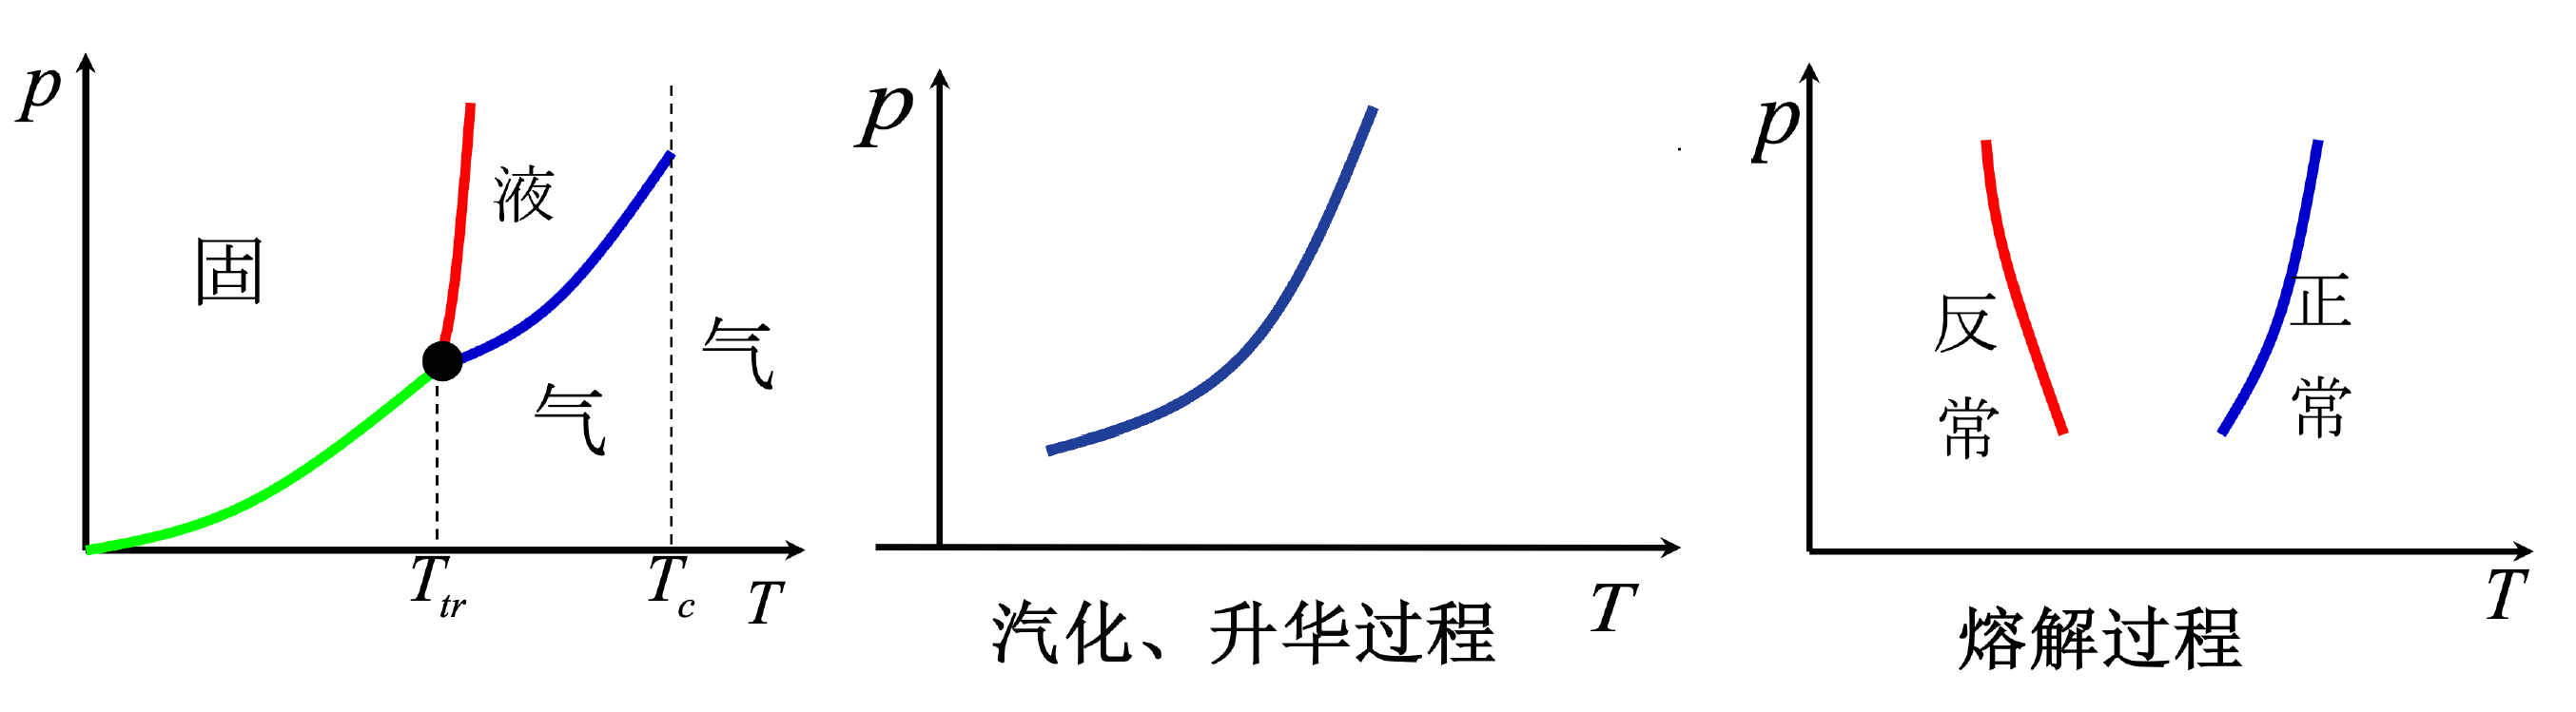
\includegraphics[width=0.7\textwidth]{phase_diagram_types.png}
\caption{常见物质相平衡曲线示意图（需插入原PPT第22次课第11页图片）}
\label{fig:phase_diagram_types}
\end{figure}

\textbf{汽化、升华过程}：大多数物质的汽化曲线和升华曲线斜率均为正，即随温度升高，饱和蒸气压增大。

\textbf{熔解过程}：
\begin{itemize}
\item \textbf{正常物质}（如$\mathrm{CO_2}$等）：熔解曲线斜率为正，即压强增大时熔点升高，$\mathrm{d}p/\mathrm{d}T>0$；
\item \textbf{反常物质}（如水）：熔解曲线斜率为负，即压强增大时熔点降低，$\mathrm{d}p/\mathrm{d}T<<0$。这是由于冰的摩尔体积大于水的摩尔体积（$V_{\text{冰}}>V_{\text{水}}$），由克拉珀龙方程$\mathrm{d}p/\mathrm{d}T=\Lambda_m/[T(V_{\beta,m}-V_{\alpha,m})]$直接得到负值。
\end{itemize}

相图上的特征点：
\begin{itemize}
\item \textbf{三相点}$\Theta$（$T_{tr}$）：固、液、气三相共存的状态；
\item \textbf{临界点}$K$（$T_c$）：液--气相变的终点，高于此温度不存在液气共存状态。
\end{itemize}


% --------------------------------------------
\subsection{二级相变相平衡曲线的斜率}
% --------------------------------------------

对于二级相变，由于相变时$S_{\beta,m}=S_{\alpha,m}$且$V_{\beta,m}=V_{\alpha,m}$，克拉珀龙方程的分子分母同时为零，成为$0/0$型不定式。此时需用洛必达法则求极限。

\paragraph{对分子、分母都求关于$T$的偏导数}

由克拉珀龙方程
\begin{equation}
\frac{\mathrm{d}p}{\mathrm{d}T}
= \frac{S_{\beta,m}-S_{\alpha,m}}{V_{\beta,m}-V_{\alpha,m}},
\end{equation}
分子分母分别对$T$求偏导（保持$p$不变）：
\begin{equation}
\frac{\mathrm{d}p}{\mathrm{d}T}
= \frac{\displaystyle\Bigl(\frac{\partial S_{\beta,m}}{\partial T}\Bigr)_p-\Bigl(\frac{\partial S_{\alpha,m}}{\partial T}\Bigr)_p}
{\displaystyle\Bigl(\frac{\partial V_{\beta,m}}{\partial T}\Bigr)_p-\Bigl(\frac{\partial V_{\alpha,m}}{\partial T}\Bigr)_p}.
\end{equation}

利用
\begin{equation}
\Bigl(\frac{\partial S_m}{\partial T}\Bigr)_p = \frac{C_{p,m}}{T},\qquad
\Bigl(\frac{\partial V_m}{\partial T}\Bigr)_p = V_m\alpha,
\end{equation}
其中$C_{p,m}$为定压摩尔热容，$\alpha$为体膨胀系数，代入得
\begin{equation}
\boxed{\frac{\mathrm{d}p}{\mathrm{d}T}
= \frac{C_{p,m,\beta}-C_{p,m,\alpha}}{T\,V_m(\alpha_\beta-\alpha_\alpha)}}
\end{equation}

\paragraph{对分子、分母都求关于$p$的偏导数}

同理，分子分母分别对$p$求偏导（保持$T$不变）：
\begin{equation}
\frac{\mathrm{d}p}{\mathrm{d}T}
= \frac{\displaystyle\Bigl(\frac{\partial S_{\beta,m}}{\partial p}\Bigr)_T-\Bigl(\frac{\partial S_{\alpha,m}}{\partial p}\Bigr)_T}
{\displaystyle\Bigl(\frac{\partial V_{\beta,m}}{\partial p}\Bigr)_T-\Bigl(\frac{\partial V_{\alpha,m}}{\partial p}\Bigr)_T}.
\end{equation}

利用麦克斯韦关系$\displaystyle\Bigl(\frac{\partial S_m}{\partial p}\Bigr)_T=-\Bigl(\frac{\partial V_m}{\partial T}\Bigr)_p=-V_m\alpha$，以及等温压缩系数$\displaystyle\kappa_T=-\frac{1}{V_m}\Bigl(\frac{\partial V_m}{\partial p}\Bigr)_T$，得
\begin{equation}
\boxed{\frac{\mathrm{d}p}{\mathrm{d}T}
= \frac{\alpha_\beta-\alpha_\alpha}{\kappa_{T,\beta}-\kappa_{T,\alpha}}}
\end{equation}

\paragraph{埃伦费斯特方程}

联立以上两式，得到\textbf{埃伦费斯特方程}（Ehrenfest equations）：
\begin{equation}
\boxed{\frac{\mathrm{d}p}{\mathrm{d}T}
= \frac{C_{p,m,\beta}-C_{p,m,\alpha}}{T\,V_m(\alpha_\beta-\alpha_\alpha)}
= \frac{\alpha_\beta-\alpha_\alpha}{\kappa_{T,\beta}-\kappa_{T,\alpha}}}
\end{equation}
这是描述二级相变相平衡曲线斜率的基本方程。


% --------------------------------------------
\subsection{一级相变及其基本特征}
% --------------------------------------------

\subsubsection*{常见一级相变概述}

\begin{itemize}
\item \textbf{液--气相变}：物质由液相转变为气相的过程称为\textbf{汽化}（蒸发、沸腾），所需能量为\textbf{汽化热}；由气相转变为液相的过程称为\textbf{凝结}，释放\textbf{凝结热}。液气相变达到相平衡时，处于气相的蒸气称为\textbf{饱和蒸气}，其压强称为\textbf{饱和蒸气压}。

\item \textbf{固--液相变}：物质由固相转变为液相的过程称为\textbf{熔解}，所需能量为\textbf{熔解热}；从液相转变为固相的过程称为\textbf{凝固}（若凝固后的固态为晶体，则称为\textbf{结晶}），释放\textbf{凝固热}。

\item \textbf{固--气相变}：物质由固相直接转变为气相的过程称为\textbf{升华}（如樟脑），所需能量为\textbf{升华热}；从气相直接转变为固相的过程称为\textbf{凝华}（如霜的形成），释放\textbf{凝华热}。固、气两相达到平衡时，固体外的蒸气压强称为\textbf{固气两相平衡的饱和蒸气压}。
\end{itemize}

\subsubsection*{饱和蒸气压与饱和蒸气压方程}

由克拉珀龙方程
\begin{equation}
\frac{\mathrm{d}p}{\mathrm{d}T}
= \frac{\Lambda_m}{T\,(V_{\beta,m}-V_{\alpha,m})}.
\end{equation}

相平衡时两相的摩尔吉布斯函数相等：
\begin{equation}
G_\alpha^{\mathrm{mol}}(T,p)=G_\beta^{\mathrm{mol}}(T,p).
\end{equation}

摩尔相变潜热
\begin{equation}
\Lambda^{\mathrm{mol}}
= T\bigl(S_\beta^{\mathrm{mol}}-S_\alpha^{\mathrm{mol}}\bigr)
= H_\beta^{\mathrm{mol}}(T)-H_\alpha^{\mathrm{mol}}(T)
= \Delta H^{\mathrm{mol}}(T_0)+\int_{T_0}^{T}\Delta C_p^{\mathrm{mol}}(T')\,\mathrm{d}T',
\end{equation}
其中
\begin{equation}
\Delta H^{\mathrm{mol}}(T_0)=H_\beta^{\mathrm{mol}}(T_0)-H_\alpha^{\mathrm{mol}}(T_0),\qquad
\Delta C_p^{\mathrm{mol}}(T)=C_{p,\beta}^{\mathrm{mol}}(T)-C_{p,\alpha}^{\mathrm{mol}}(T).
\end{equation}

若$\Delta C_p^{\mathrm{mol}}$在一定温区内可近似为常量，则
\begin{equation}
\Lambda^{\mathrm{mol}}
= \Delta H^{\mathrm{mol}}(T_0)+\Delta C_p^{\mathrm{mol}}\cdot(T-T_0).
\end{equation}

\paragraph{气--液相变的简化}

气--液相变中$V_\beta^{\mathrm{mol}}\gg V_\alpha^{\mathrm{mol}}$，且气相可近似为理想气体$V_\beta^{\mathrm{mol}}=RT/p$，于是
\begin{equation}
\frac{\mathrm{d}p}{\mathrm{d}T}
= \frac{\Lambda^{\mathrm{mol}}}{T\,V_\beta^{\mathrm{mol}}}
= \frac{p\,\Lambda^{\mathrm{mol}}}{R\,T^2},
\qquad
\frac{\mathrm{d}p}{p}
= \frac{\Lambda^{\mathrm{mol}}\,\mathrm{d}T}{R\,T^2}.
\end{equation}

积分得\textbf{饱和蒸气压方程}：
\begin{equation}
\boxed{\ln\frac{p}{p_0}
= B\Bigl(1-\frac{T_0}{T}\Bigr)+C\ln\frac{T}{T_0}}
\end{equation}
其中
\begin{equation}
B=\frac{\Delta H^{\mathrm{mol}}(T_0)-\Delta C_p^{\mathrm{mol}}T_0}{R\,T_0},
\qquad
C=\frac{\Delta C_p^{\mathrm{mol}}}{R}.
\end{equation}

当温度在很小范围内变化时，摩尔相变潜热$\Lambda^{\mathrm{mol}}$可近似为常量，则
\begin{equation}
\frac{\mathrm{d}p}{\mathrm{d}T}
= \frac{\Lambda^{\mathrm{mol}}}{T\,V_\beta^{\mathrm{mol}}}
= \frac{p\,\Lambda^{\mathrm{mol}}}{R\,T^2},
\end{equation}
积分得近似公式
\begin{equation}
\boxed{p \approx p_0\,\exp\!\Bigl(\frac{\Lambda^{\mathrm{mol}}}{R\,T_0}\Bigr)\cdot\exp\!\Bigl(-\frac{\Lambda^{\mathrm{mol}}}{R\,T}\Bigr)}
\end{equation}
即饱和蒸气压随温度升高呈指数增长。

\subsubsection*{液气相变的微观解释}

设在一定温度下液气两相达到平衡，此时系统压强为$p$。一个液态分子从液态表面跃出需要两部分能量：
\begin{enumerate}
\item 克服液体内部其他分子对它的吸引力；
\item 对抗液面上已经形成的蒸气压做功。
\end{enumerate}

为维持系统温度不变，外界必须给系统提供能量，即\textbf{汽化潜热}
\begin{equation}
\lambda = \Delta u + p\,\Delta v = T(s_g-s_l).
\end{equation}

对一摩尔分子：
\begin{equation}
\Lambda_{\mathrm{mol}} = \Delta U_{\mathrm{mol}}+p\,\Delta V_{\mathrm{mol}}
= T\bigl(S_{\mathrm{mol},g}-S_{\mathrm{mol},l}\bigr).
\end{equation}

\paragraph{分子蒸发与凝结的动态平衡}

把液体看成是数密度为$n_l$的气体，用$u$表示分子速度在垂直液面方向的分量。则处于$u\sim u+\mathrm{d}u$的液体分子数为
\begin{equation}
\mathrm{d}n_l = n_l f(u)\,\mathrm{d}u.
\end{equation}

限定只有动能大于汽化潜热的分子才能跃出液面，则单位时间从单位面积上跃出液面的分子数为
\begin{equation}
n_l\Bigl(\frac{m}{2\pi k_BT}\Bigr)^{1/2}\int_{\sqrt{2\lambda/m}}^{\infty}
u\,\exp\!\Bigl(-\frac{mu^2}{2k_BT}\Bigr)\,\mathrm{d}u
= n_l\Bigl(\frac{k_BT}{2\pi m}\Bigr)^{1/2}\exp\!\Bigl(-\frac{\lambda}{k_BT}\Bigr).
\end{equation}

设$n_g$为蒸气的分子数密度，单位时间碰到单位面积的分子数为
\begin{equation}
\frac{1}{4}n_g\bar{v}
= n_g\Bigl(\frac{k_BT}{2\pi m}\Bigr)^{1/2}.
\end{equation}

平衡时跃出与凝结的分子数相等（设凝结系数为$\alpha$）：
\begin{equation}
n_l\exp\!\Bigl(-\frac{\lambda}{k_BT}\Bigr)
= \alpha\,n_g.
\end{equation}

由理想气体状态方程$p=n_gk_BT$，得饱和蒸气压
\begin{equation}
p = n_gk_BT
= \Bigl(\frac{n_lk_BT}{\alpha}\Bigr)\exp\!\Bigl(-\frac{\Lambda_{\mathrm{mol}}}{RT}\Bigr),
\end{equation}
即
\begin{equation}
\ln p = -\frac{\Lambda_{\mathrm{mol}}}{RT}+\ln T+\ln\!\Bigl(\frac{k_Bn_l}{\alpha}\Bigr).
\end{equation}

这与宏观推导的饱和蒸气压方程$\displaystyle\ln\frac{p}{p_0}=B\bigl(1-\frac{T_0}{T}\bigr)+C\ln\frac{T}{T_0}$在形式上完全一致，建立了微观机制与宏观热力学之间的联系。


% --------------------------------------------
\subsection{相平衡曲线与临界现象}
% --------------------------------------------

\subsubsection*{安德鲁斯实验结果（1869年）}

安德鲁斯对$\mathrm{CO_2}$的等温线进行实验测量，得到以下重要结果（如图所示）：

\begin{figure}[htbp]
\centering
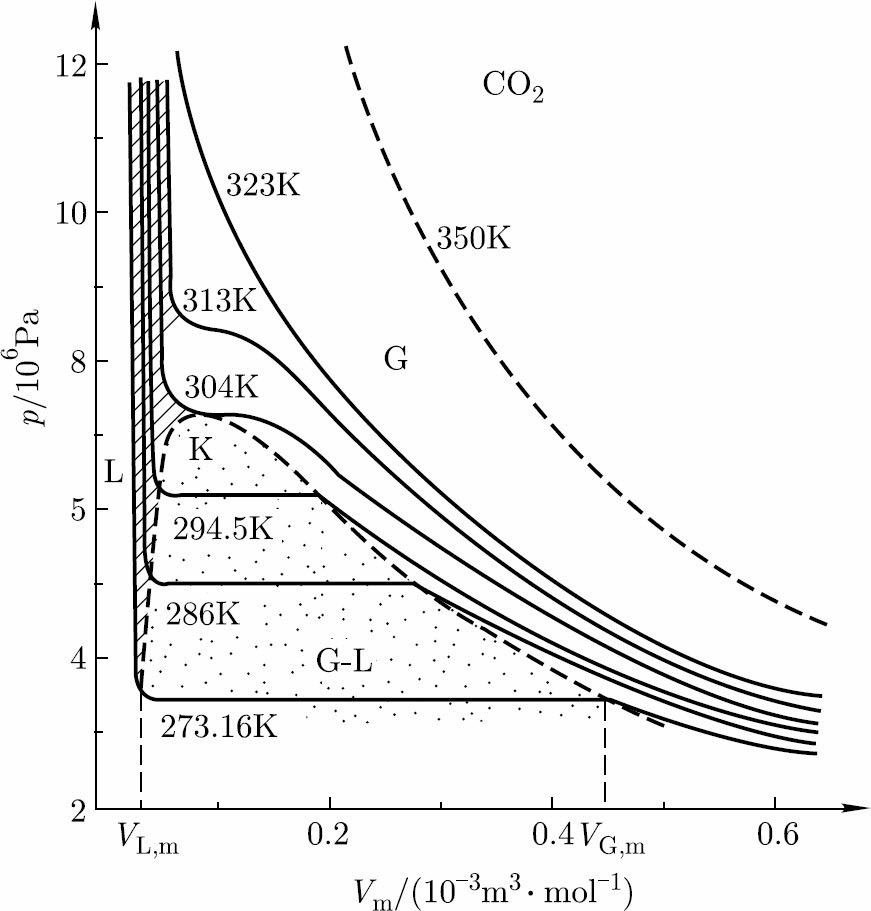
\includegraphics[width=0.5\textwidth]{andrews_co2.png}
\caption{$\mathrm{CO_2}$的安德鲁斯实验等温线（需插入原PPT第22次课第14页图片）}
\label{fig:andrews}
\end{figure}

\begin{itemize}
\item 温度较低时，$p$-$V$空间分为三部分：液体、气体、液气共存；
\item 随着温度升高，液气共存区逐渐减小，两相的摩尔体积差别逐渐减小；
\item 温度升高到\textbf{临界温度}$T_c$时，水平的等压线缩为一个点，$V_{L,m}=V_{G,m}$；
\item 温度高于$T_c$时（如$T=350\,\mathrm{K}$），$\mathrm{CO_2}$的等温线接近理想气体的等温线；
\item 其它物质的等温线也都有完全相同的特征。
\end{itemize}

\subsubsection*{范德瓦尔斯等温线的理论描述}

范德瓦尔斯方程
\begin{equation}
\Bigl(p+\frac{a}{V_m^2}\Bigr)(V_m-b)=RT
\quad\Longrightarrow\quad
V_m^3-\Bigl(b+\frac{RT}{p}\Bigr)V_m^2+\frac{a}{p}V_m-\frac{ab}{p}=0.
\end{equation}

给定$p,T$时，$V_m$的解有四种情况：

\begin{enumerate}
\item[(I)] \textbf{三个不等的实根}：对应液气相平衡共存状态；
\item[(II)] \textbf{三个实根，其中两个相等}：对应单相--双相转变点；
\item[(III)] \textbf{三个相等实根}：对应\textbf{临界点}；
\item[(IV)] \textbf{一个实根、两个虚根}：对应单相（超临界流体或单一气相/液相）。
\end{enumerate}

\begin{figure}[htbp]
\centering
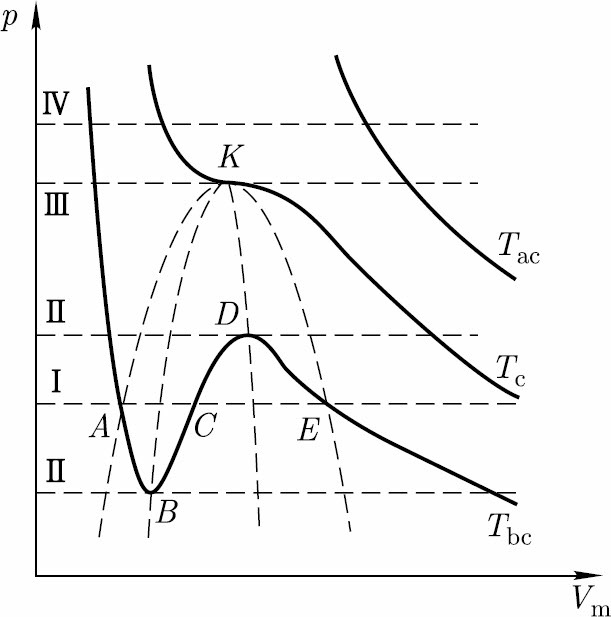
\includegraphics[width=0.45\textwidth]{van_der_waals_isotherms.png}
\caption{范德瓦尔斯等温线示意图（需插入原PPT第22次课第15页图片）}
\label{fig:vdw_isotherms}
\end{figure}

图中各特征点与线：
\begin{itemize}
\item $T_{bc}$：低于临界温度的等温线，出现液气共存平台（$AB$段为液体，$DE$段为气体，$BD$间为不稳定区）；
\item $T_c$：临界等温线，在临界点$K$处出现拐点，$(\partial p/\partial V)_T=0$且$(\partial^2p/\partial V^2)_T=0$；
\item $T_{ac}$：高于临界温度的等温线，接近理想气体行为；
\item 虚线$AKB$：实际相变时液气共存的平台边界（麦克斯韦等面积法则）。
\end{itemize}

\textbf{问题}：范德瓦尔斯方程本身在$BD$区域给出$(\partial p/\partial V)_T>0$的不稳定状态，实际不存在等压段，需要用\textbf{麦克斯韦等面积法则}修正，使平台$AB$与$DE$之间的面积相等，以确定真实的相变压强。

% --------------------------------------------
\subsection{等压线的确定与杠杆原理}
% --------------------------------------------

\subsubsection*{Maxwell等面积法则}

对于范德瓦尔斯等温线，曲线$ABCDE$中水平直线段$ACE$是液气共存的等压线。相平衡要求两端化学势相等：
\begin{equation}
\mu_A = \mu_E.
\end{equation}

由于$\mu = G^{\mathrm{mol}} = F^{\mathrm{mol}} + pV^{\mathrm{mol}}$，有
\begin{align}
\mu_A &= F_A^{\mathrm{mol}} + p^*V_L^{\mathrm{mol}},\\
\mu_E &= F_E^{\mathrm{mol}} + p^*V_G^{\mathrm{mol}}.
\end{align}

由$\mu_A=\mu_E$得
\begin{equation}
F_A^{\mathrm{mol}} - F_E^{\mathrm{mol}} = p^*\bigl(V_G^{\mathrm{mol}}-V_L^{\mathrm{mol}}\bigr).
\end{equation}

在准静态等温条件下$\mathrm{d}F^{\mathrm{mol}}=-p\,\mathrm{d}V^{\mathrm{mol}}$，故
\begin{equation}
F_A^{\mathrm{mol}}-F_E^{\mathrm{mol}} = -\int_{F_E^{\mathrm{mol}}}^{F_A^{\mathrm{mol}}}\mathrm{d}F
= \int_{ABCDE}p\,\mathrm{d}V^{\mathrm{mol}}.
\end{equation}

比较两式可知，等压线高度$p^*$必须满足
\begin{equation}
\int_{ABCDE}p\,\mathrm{d}V^{\mathrm{mol}} = p^*\bigl(V_G^{\mathrm{mol}}-V_L^{\mathrm{mol}}\bigr).
\end{equation}

这等价于\textbf{Maxwell等面积法则}：水平线段$ACE$的高度$p^*$由曲边形$ABCA$的面积与曲边形$CDEC$的面积相等确定，即
\begin{equation}
\boxed{\int_{V_L^{\mathrm{mol}}}^{V_G^{\mathrm{mol}}}p\,\mathrm{d}V^{\mathrm{mol}} - p^*\bigl(V_G^{\mathrm{mol}}-V_L^{\mathrm{mol}}\bigr)=0}
\end{equation}
或表述为：等温线上曲线与等压线围成的两区域面积相等。

\begin{figure}[htbp]
\centering
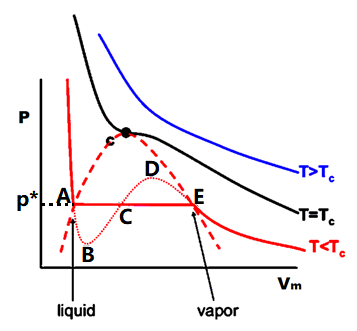
\includegraphics[width=0.45\textwidth]{maxwell_construction.png}
\caption{Maxwell等面积法则示意图（需插入原PPT第23次课第4页图片）}
\label{fig:maxwell}
\end{figure}

\subsubsection*{相平衡时两相的物质的量之间的关系（杠杆原理）}

以液气相变为例，设液相和气相的摩尔体积分别为$V_L^{\mathrm{mol}}$和$V_G^{\mathrm{mol}}$，两相平衡时系统的平均摩尔体积为$\bar{V}$。定义两相的摩尔分数
\begin{equation}
x_L=\frac{V_L}{V},\qquad x_G=\frac{V_G}{V},
\end{equation}
其中$V_L$、$V_G$分别为液相、气相占据的总体积，$V$为系统总体积。

由总体积守恒和摩尔分数归一化：
\begin{equation}
x_G V_G^{\mathrm{mol}} + x_L V_L^{\mathrm{mol}} = \bar{V},\qquad x_G+x_L=1.
\end{equation}

解得
\begin{equation}
\boxed{x_L=\frac{V_G^{\mathrm{mol}}-\bar{V}}{V_G^{\mathrm{mol}}-V_L^{\mathrm{mol}}},\qquad
x_G=\frac{\bar{V}-V_L^{\mathrm{mol}}}{V_G^{\mathrm{mol}}-V_L^{\mathrm{mol}}}}
\end{equation}

或写成
\begin{equation}
\boxed{x_G\bigl(V_G^{\mathrm{mol}}-\bar{V}\bigr)=x_L\bigl(\bar{V}-V_L^{\mathrm{mol}}\bigr)}
\end{equation}

此即\textbf{杠杆原理}：一级相变平衡时两相物质的摩尔百分比满足杠杆原理，系统平均摩尔体积$\bar{V}$相当于杠杆支点。

\begin{figure}[htbp]
\centering
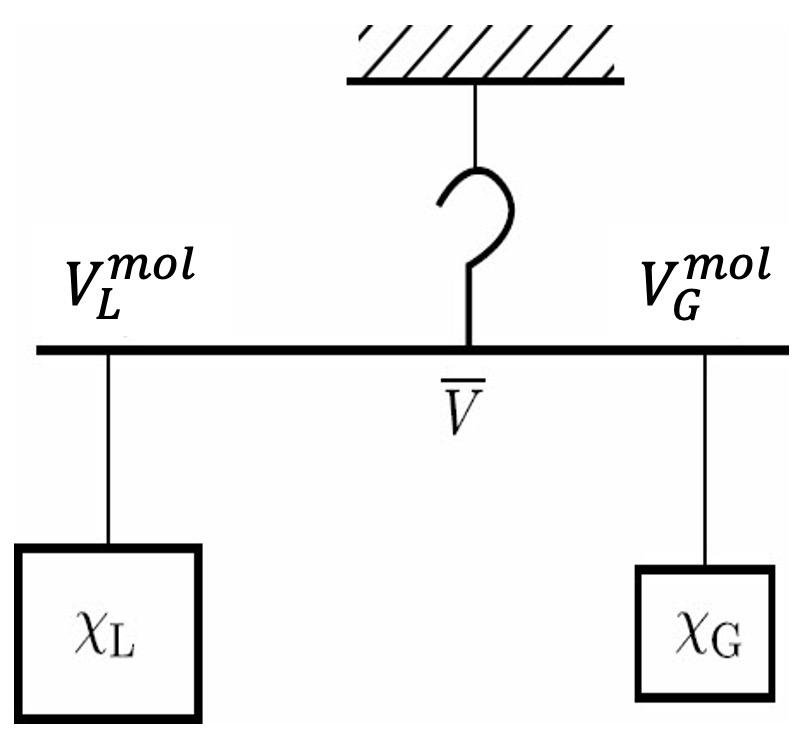
\includegraphics[width=0.4\textwidth]{lever_rule.png}
\caption{杠杆原理示意图（需插入原PPT第23次课第5页图片）}
\label{fig:lever}
\end{figure}

% --------------------------------------------
\subsection{热力学函数的特征与两相共存条件}
% --------------------------------------------

\subsubsection*{相平衡时的自由能}

以液气相变系统为例，设相平衡时温度固定为$T$，系统总体积$V=\nu\bar{V}$。记$F_G$、$F_L$分别为系统处于纯气相、纯液相时的摩尔自由能，$x_G$、$x_L$分别为气相、液相的摩尔百分比。则系统的总摩尔自由能为
\begin{equation}
F = x_G F_G + x_L F_L.
\end{equation}

将杠杆原理代入，得
\begin{equation}
F = \frac{\bar{V}-V_L^{\mathrm{mol}}}{V_G^{\mathrm{mol}}-V_L^{\mathrm{mol}}}F_G
+ \frac{V_G^{\mathrm{mol}}-\bar{V}}{V_G^{\mathrm{mol}}-V_L^{\mathrm{mol}}}F_L.
\end{equation}

整理可得
\begin{equation}
\bigl(V_G^{\mathrm{mol}}-V_L^{\mathrm{mol}}\bigr)(F-F_G)
= \bigl(V_G^{\mathrm{mol}}-\bar{V}\bigr)(F_L-F_G),
\end{equation}
即
\begin{equation}
\frac{F-F_G}{V_G^{\mathrm{mol}}-\bar{V}} = \frac{F_L-F_G}{V_G^{\mathrm{mol}}-V_L^{\mathrm{mol}}}.
\end{equation}

\textbf{结论}：在（相分离）相平衡时，代表总摩尔自由能大小的点$P(\bar{V},F)$一定在$P_G(V_G^{\mathrm{mol}},F_G)$和$P_L(V_L^{\mathrm{mol}},F_L)$的连线上。

\begin{figure}[htbp]
\centering
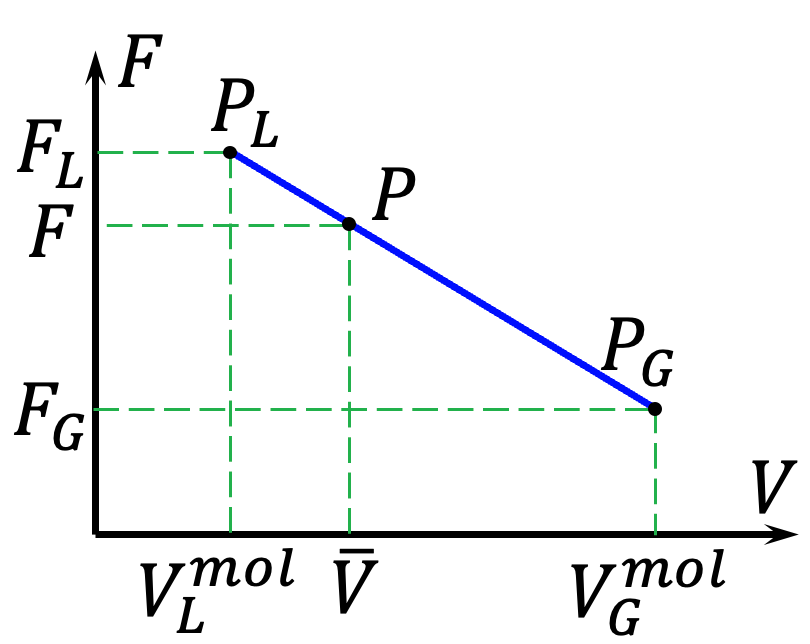
\includegraphics[width=0.45\textwidth]{free_energy_two_phase.png}
\caption{相平衡时自由能的线性组合特征（需插入原PPT第23次课第6--7页图片）}
\label{fig:free_energy_two_phase}
\end{figure}

\subsubsection*{两相共存的可能性与自由能曲线}

自由能曲线的几何形状决定了两相共存是否可能出现：

\begin{itemize}
\item \textbf{情形（a）——单相稳定}：若自由能曲线$F(V)$在整个范围内均为凹函数（$\mathrm{d}^2F/\mathrm{d}V^2>0$），则无论$\bar{V}$、$V_G^{\mathrm{mol}}$、$V_L^{\mathrm{mol}}$取何值，总有$F_2>F_1$（$F_1$为单相自由能，$F_2$为假想两相混合自由能）。因此单相自由能更小，\textbf{单相是平衡态}，不出现两相共存。

\item \textbf{情形（b）——两相共存可能}：若自由能曲线两端凹、中间凸（$\mathrm{d}^2F/\mathrm{d}V^2<<0$），则存在区间使得$F_2<F_1$。此时\textbf{可能出现两相共存}（相分离）。
\end{itemize}

\begin{figure}[htbp]
\centering
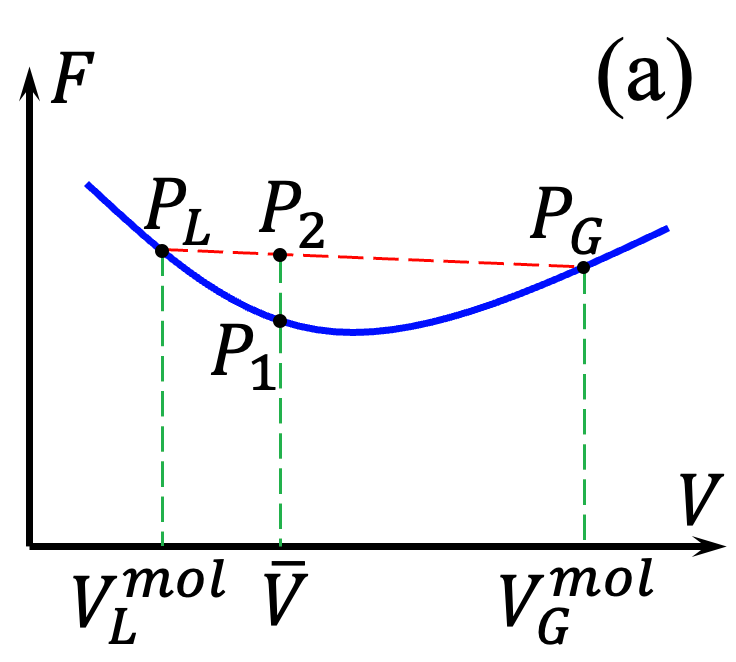
\includegraphics[width=0.45\textwidth]{free_energy_convexity_a.png}
\caption{自由能曲线凹性对相共存的影响（需插入原PPT第23次课第8页图片）}
\label{fig:convexity_a}
\end{figure}

\begin{figure}[htbp]
    \centering
    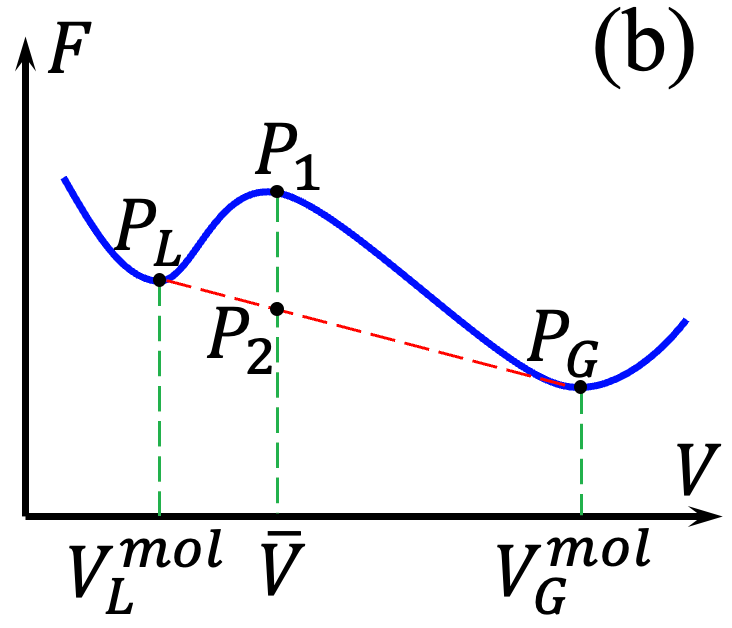
\includegraphics[width=0.45\textwidth]{free_energy_convexity_b.png}
    \caption{自由能曲线凸性对相共存的影响（需插入原PPT第23次课第8页图片）}
    \label{fig:convexity_b}
\end{figure}


其中蓝线表示单相变化的等温线（如范德瓦尔斯等温线），红线表示两相共存（或出现相分离）的等温线。

% --------------------------------------------
\subsection{相变的方式：失稳分解与成核长大}
% --------------------------------------------

\subsubsection*{自由能曲线的拐点与相图分区}

对于有两相共存可能性的系统，自由能曲线中间上凸、两端上凹，中间存在两个拐点$S$和$S'$。根据自由能曲线的形状，可将相图分为三个部分：
\begin{itemize}
\item $P_L S$：液相侧亚稳区；
\item $SS'$：失稳区（上凸区）；
\item $S'P_G$：气相侧亚稳区。
\end{itemize}

\subsubsection*{体积（密度）涨落的影响}

考虑系统在体积$V$处发生对称涨落$\pm\Delta V$，两相混合后的自由能近似为
\begin{equation}
F_2 = \frac{1}{2}\bigl[F_1(V+\Delta V)+F_1(V-\Delta V)\bigr]
\approx F_1(V) + \frac{1}{2}\frac{\mathrm{d}^2F_1}{\mathrm{d}V^2}(\Delta V)^2.
\end{equation}

\textbf{相分离判据}：若$F_2<F_1$，即
\begin{equation}
\boxed{\frac{\mathrm{d}^2F}{\mathrm{d}V^2}<0}
\end{equation}
则任意小的密度涨落都导致自由能下降，系统自发分离为两相。

\subsubsection*{失稳分解（Spinodal Decomposition）}

对于上凸区（$SS'$），由于$\mathrm{d}^2F/\mathrm{d}V^2<<0$，\textbf{任意小的密度涨落都导致自由能下降}，系统无需克服势垒即可自发分解为两相，最终达到两相分离的稳定态。这种由单相分解成两相的方式称为\textbf{失稳分解}。

\subsubsection*{亚稳态与成核长大（Nucleation and Growth）}

当体积处于$\mathrm{d}^2F/\mathrm{d}V^2>0$的区域（$P_L S$或$S'P_G$）时，对于小的体积变化$\Delta V$有$F_2>F_1$。在该区域内的分解\textbf{可以不发生}，故称此时的系统为\textbf{亚稳态}。

\begin{itemize}
\item \textbf{过热液体}：对于亚稳区$P_L S$，从温度看液体可以汽化，但未能汽化，称之为过热液体。
\item \textbf{过冷蒸气}：对于亚稳区$S'P_G$，气体可以液化但未能液化，称之为过冷蒸气。
\end{itemize}

但小范围的涨落可在一相中形成另一相的\textbf{核}，然后逐渐扩大范围形成两相。这种由单相到两相的过渡称为\textbf{成核长大}。

\begin{figure}[htbp]
\centering
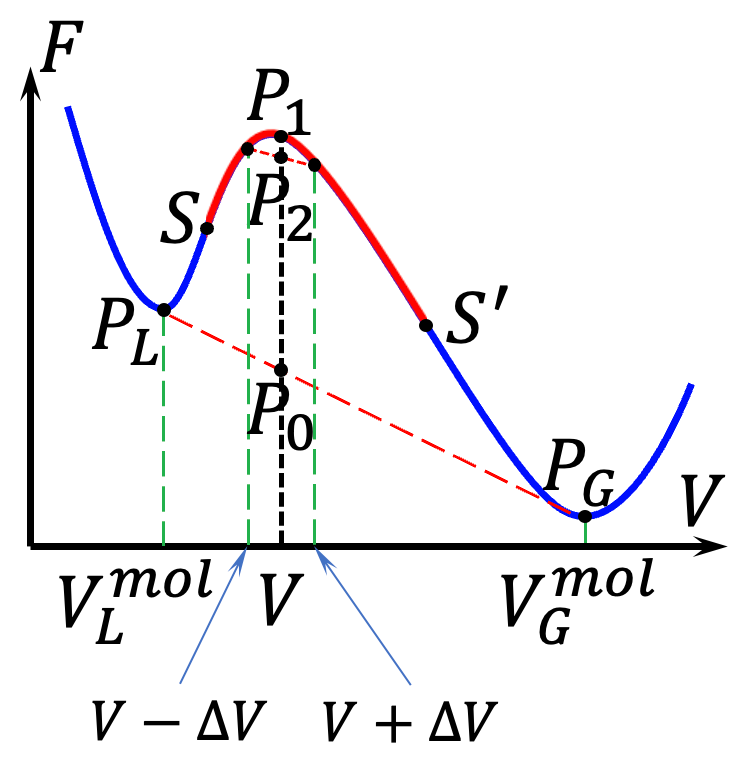
\includegraphics[width=0.45\textwidth]{phase_transition_modes.png}
\caption{相变方式：失稳分解与成核长大（需插入原PPT第23次课第9--10页图片）}
\label{fig:phase_modes}
\end{figure}

\begin{remark}
失稳分解与成核长大的本质区别：
\begin{itemize}
\item \textbf{失稳分解}：发生在自由能曲线的失稳区（$\mathrm{d}^2F/\mathrm{d}V^2<<0$），无需克服势垒，由无限小的涨落触发，相变在整个系统中均匀发生。
\item \textbf{成核长大}：发生在亚稳区（$\mathrm{d}^2F/\mathrm{d}V^2>0$），需要克服成核势垒形成临界尺寸的核，然后核逐渐长大。
\end{itemize}
\end{remark}

% --------------------------------------------
\subsection{失稳分解区与成核长大区在\texorpdfstring{$p$-$V$}{p-V}图上的图示}
% --------------------------------------------

\subsubsection*{\texorpdfstring{$p$-$V$}{p-V}图上的分区}

由相分离判据$\mathrm{d}^2F/\mathrm{d}V^2<<0$及热力学关系
\begin{equation}
\left(\frac{\partial^2F}{\partial V^2}\right)_T=-\left(\frac{\partial p}{\partial V}\right)_T,
\end{equation}
可知自由能曲线的拐点对应于$p$-$V$图等温线上满足$(\partial p/\partial V)_T=0$的极值点。

在$p$-$V$图上，各特征区域划分如下：
\begin{itemize}
\item \textbf{失稳曲线}（Spinodal曲线）：将各等温线上满足$(\partial p/\partial V)_T=0$的极值点连接而成的曲线。该曲线所包围的中间区域即为\textbf{失稳分解区}。
\item \textbf{相平衡曲线}（Binodal曲线）：将各等温线上气液两相平衡共存的端点（即$V_L^{\mathrm{mol}}$与$V_G^{\mathrm{mol}}$）连接而成的曲线，即通常的液气相平衡边界。
\item \textbf{成核长大区}（亚稳区）：失稳曲线与相平衡曲线之间的区域。在此区域内系统处于亚稳态，需要克服成核势垒才能发生相变。
\end{itemize}

\begin{figure}[htbp]
\centering
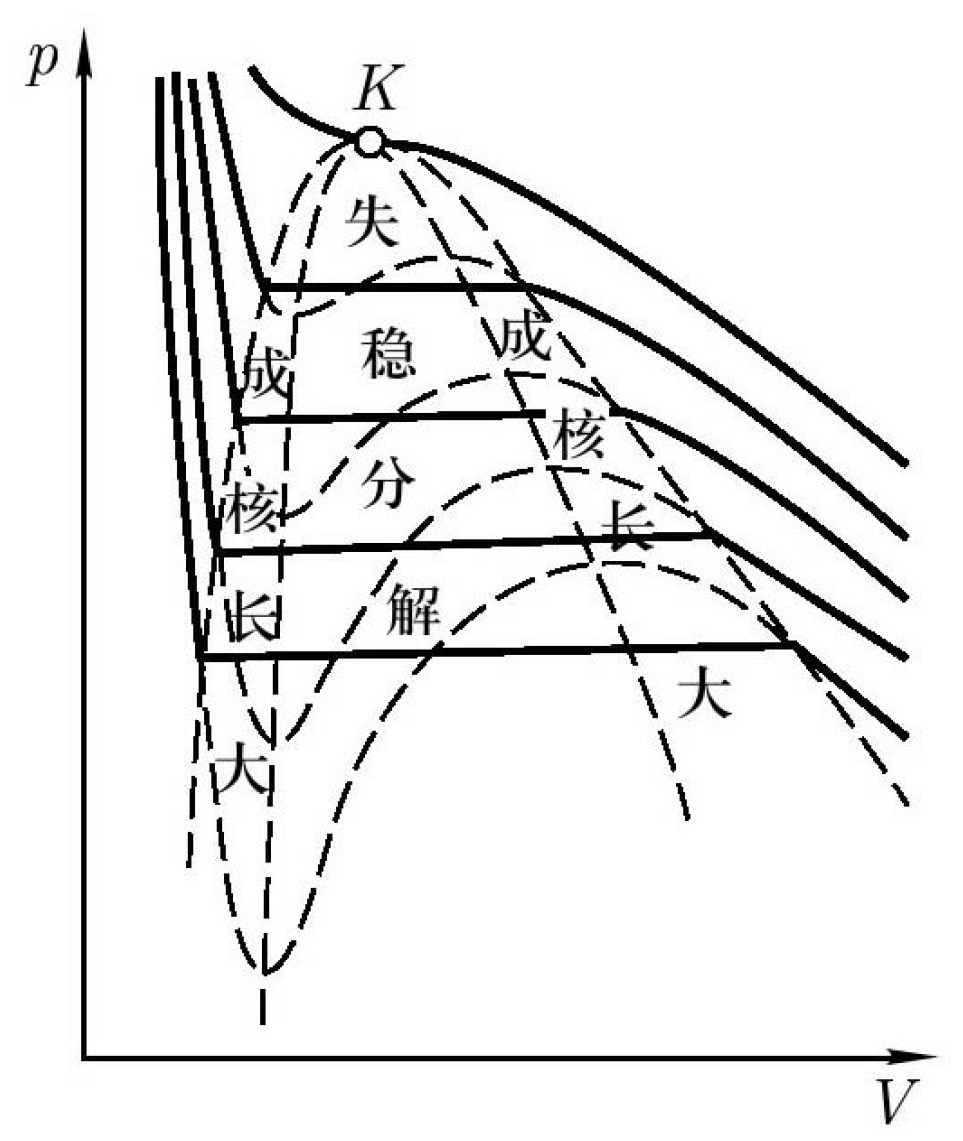
\includegraphics[width=0.45\textwidth]{spinodal_binodal_pv.png}
\caption{$p$-$V$图上的失稳分解区与成核长大区（需插入原PPT第23次课第11--12页图片）}
\label{fig:spinodal_pv}
\end{figure}

\begin{remark}
一级相变均存在这种亚稳态的情况。在失稳分解区内，任意小的密度涨落都使系统自由能下降，从而自发分离为两相；在成核长大区内，系统需要先有足够大的涨落形成临界核，才能逐渐长大实现相变。
\end{remark}

% --------------------------------------------
\subsection{弯曲液面对气-液相变的影响}
% --------------------------------------------

\subsubsection*{弯曲液面下的相平衡条件}

设平液面上液气相变达到平衡时，饱和蒸气的温度、压强分别为$T$、$p$，则相平衡条件为
\begin{equation}
\mu_g(p,T)=\mu_l(p,T).
\end{equation}

当在液体中形成半径为$R$的球形气泡时，由于表面张力的存在，气泡内外存在压强差。设气泡内（气相）压强为$p'$，温度为$T'$；则气泡外紧邻液面的压强为$p'-2\alpha/R$（$\alpha$为表面张力系数）。此时相平衡条件为
\begin{equation}
\mu_g(p',T')=\mu_l\!\left(p'-\frac{2\alpha}{R},T'\right).
\end{equation}

\begin{figure}[htbp]
\centering
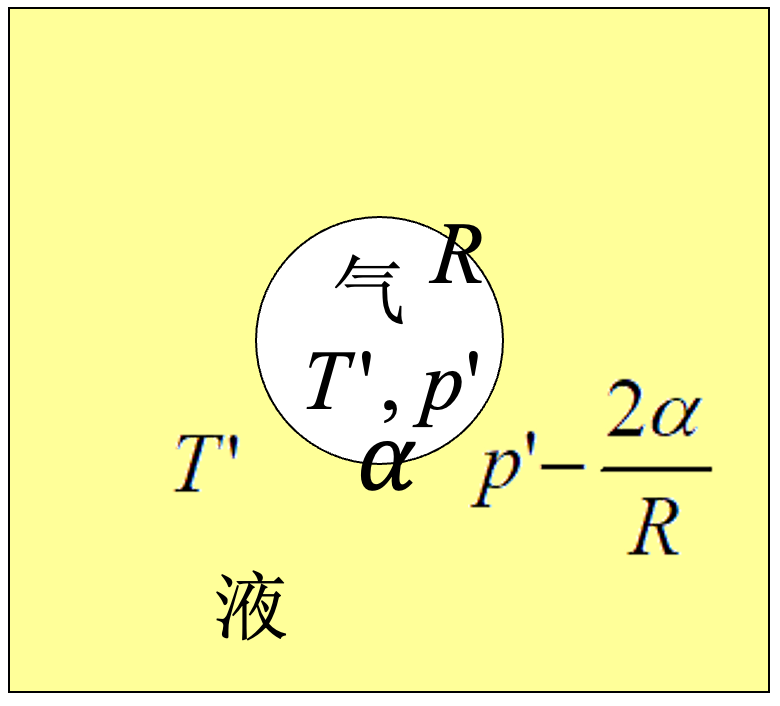
\includegraphics[width=0.25\textwidth]{bubble_phase_equilibrium.png}
\caption{液体中球形气泡的相平衡示意图（需插入原PPT第23次课第14页图片）}
\label{fig:bubble_equilibrium}
\end{figure}

\subsubsection*{弯曲液面饱和蒸气压的推导}

利用$\mathrm{d}G^{\mathrm{mol}}=V^{\mathrm{mol}}\,\mathrm{d}p-S^{\mathrm{mol}}\,\mathrm{d}T$，在压强、温度变化不大的条件下展开：

\textbf{气相}：
\begin{equation}
\mu_g(p',T')-\mu_g(p,T)\approx RT\ln\frac{p'}{p}-S_g^{\mathrm{mol}}\Delta T,
\end{equation}
其中$\Delta T=T'-T$，并利用了理想气体状态方程$pV_g^{\mathrm{mol}}=RT$。

\textbf{液相}：
\begin{equation}
\mu_l\!\left(p'-\frac{2\alpha}{R},T'\right)-\mu_l(p,T)\approx\left(p'-\frac{2\alpha}{R}-p\right)V_l^{\mathrm{mol}}-S_l^{\mathrm{mol}}\Delta T,
\end{equation}
其中利用了液体摩尔体积$V_l^{\mathrm{mol}}\approx\mathrm{const}$。

联立两式，在$(p'-p)/p\ll1$的条件下（此时$\ln(p'/p)\approx(p'-p)/p=(p'-p)V_g^{\mathrm{mol}}/RT$），整理得
\begin{equation}
\boxed{(p'-p)\bigl(V_g^{\mathrm{mol}}-V_l^{\mathrm{mol}}\bigr)+\frac{2\alpha}{R}V_l^{\mathrm{mol}}=(S_g^{\mathrm{mol}}-S_l^{\mathrm{mol}})\Delta T}
\end{equation}

利用$V_l^{\mathrm{mol}}=\mu/\rho_l$、$V_g^{\mathrm{mol}}=\mu/\rho_g$（$\rho_l$、$\rho_g$为液、气相密度，$\mu$为摩尔质量），并注意到$V_g^{\mathrm{mol}}\gg V_l^{\mathrm{mol}}$，上式化为
\begin{equation}
\boxed{(p'-p)+\frac{2\alpha}{R}\frac{\rho_g}{\rho_l-\rho_g}=\frac{\Lambda}{TV_g^{\mathrm{mol}}}\Delta T}
\end{equation}
其中$\Lambda=T(S_g^{\mathrm{mol}}-S_l^{\mathrm{mol}})$为摩尔汽化热。

\subsubsection*{等温条件下的开尔文效应}

若$\Delta T=0$（等温），则
\begin{equation}
p'-p=-\frac{2\alpha}{R}\frac{\rho_g}{\rho_l-\rho_g}\approx-\frac{2\alpha}{R}\frac{\rho_g}{\rho_l}.
\end{equation}

\textbf{物理结论}（此处$R$的符号约定与部分传统教材相反：曲率中心在气相中时$R>0$，即液面为凹面）：
\begin{itemize}
\item \textbf{凹液面}（$R>0$，如液体中的气泡）：$p'<p$，凹面液体的饱和蒸气压\textbf{小于}平面液体的饱和蒸气压。
\item \textbf{凸液面}（$R<<0$，如液滴）：$p'>p$，凸面液体的饱和蒸气压\textbf{大于}平面液体的饱和蒸气压。
\end{itemize}

此即\textbf{开尔文方程}（Kelvin equation）的物理实质：弯曲液面的饱和蒸气压与平面液面不同，液滴（凸面）的饱和蒸气压更高，气泡（凹面）的饱和蒸气压更低。

% --------------------------------------------
\subsection{过热液体与临界半径}
% --------------------------------------------

\subsubsection*{过热液体的条件}

将弯曲液面公式写成
\begin{equation}
(p'-p)+\frac{2\alpha}{R}\frac{\rho_g}{\rho_l-\rho_g}=\frac{\Lambda}{TV_g^{\mathrm{mol}}}\Delta T_c,
\end{equation}
其中$\Delta T_c=T'-T$表示半径为$R$的气泡存在时与平液面相变温度的温度差。

若气泡内压强与外部饱和蒸气压相等（$p'=p$），则
\begin{equation}
\frac{2\alpha}{R}\frac{\rho_l}{\rho_l-\rho_g}=\frac{\Lambda}{TV_g^{\mathrm{mol}}}\Delta T_c,
\end{equation}
解得
\begin{equation}
\boxed{\Delta T_c=\frac{2\alpha\rho_l V_g^{\mathrm{mol}}T}{R\Lambda(\rho_l-\rho_g)}}
\end{equation}

当$R>0$（液体中存在气泡）时，$\Delta T_c>0$，说明液体需要被加热到高于正常沸点的温度才能使该气泡稳定存在，此时液体处于\textbf{过热液体}状态。

\subsubsection*{气泡的稳定性与沸腾}

设系统温度为$T+\Delta T_c$（恰好使半径$R$的气泡达到平衡）：

\begin{itemize}
\item \textbf{若气泡半径$R_1<R$}：则对应的$\Delta T_c^1>\Delta T_c$。在当前温度下，该气泡不足以稳定存在，液相物质向气相运动导致气泡收缩，最终气泡消失。
\item \textbf{若气泡半径$R_1>R$}：则对应的$\Delta T_c^1<\Delta T_c$。在当前温度下，气相物质不断向气泡聚集，气泡增大，$R$增大又使$\Delta T_c^1$进一步减小，过程加速。最终气泡克服液体粘滞力，在浮力作用下逃出液体——即\textbf{沸腾}。
\end{itemize}

\subsubsection*{临界半径（中肯半径）}

从弯曲液面相平衡公式出发，令$\Delta T=0$，定义使相变刚好能够发生的\textbf{临界半径}（又称\textbf{中肯半径}）：
\begin{equation}
\boxed{R_c=-\frac{2\alpha\rho_g}{(p'-p)(\rho_l-\rho_g)}}
\end{equation}

\textbf{物理意义}：只有当生成的核（气泡或液滴）大于临界核的大小$R_c$时，才能实现两相分离；小于临界核的涨落将自发消失。临界半径的存在解释了为什么过热液体或过冷蒸气可以在一定条件下以亚稳态存在。

\textbf{应用}：人工降雨（提供凝结核使过冷水滴长大）、威尔逊云室（过饱和蒸气在带电粒子轨迹上凝结）等。

\end{document}